% ============================================================================
% Environmental Provisions in Chinese PTAs and Export Composition
% Version 4 — reorganised results, built on paper_v3.
%
% What changed relative to v3:
%   - Section 5 rewritten and restructured from twelve subsections to five:
%       5.1 full panel  ->  5.2 collapsed panel and robust inference
%       ->  5.3 comparison groups  ->  5.4 agreement content  ->  5.5 dynamics,
%       influence and extensive margin. Green and dirty margins carried together.
%   - Main tables replaced by the verified six-column versions (three outcomes x
%       two indices, two depth-control panels). Depth control and quantity/unit
%       value are now dimensions of the tables rather than separate subsections.
%   - New compact saturation ladder (Table 2), terminating at the reference spec.
%   - Corrected table values: full-panel SE/asymptotic p in the value columns were
%       taken from the "with controls" run in the source document; collapsed panel
%       B took the depth-control rows. Both fixed against the Stata CSVs.
%   - Dirty margin re-framed: significance depends on the depth control, and the
%       permutation test is the tie-breaker. Abstract, intro and conclusion updated.
%   - Robustness moved to a restructured appendix (A-J), incl. new sections on
%       Hong Kong/Macao, alternative depth controls, CO2 intensity and dynamics.
%
% Compile: pdflatex + biber + pdflatex (x2); figures in ./figures/
% ============================================================================
\documentclass[12pt]{article}
\usepackage[T1]{fontenc}
\usepackage[utf8]{inputenc}
\usepackage{amsmath, amssymb}
\usepackage{booktabs}
\usepackage{graphicx}
\usepackage{geometry}
\geometry{margin=2.5cm}
\usepackage{setspace}
\onehalfspacing
\usepackage[bottom]{footmisc}
\usepackage[hidelinks]{hyperref}
\usepackage{threeparttable}
\usepackage{float}
\usepackage[section]{placeins}
\usepackage[style=authoryear-comp, natbib=true, backend=biber]{biblatex}
\addbibresource{references.bib}
\DeclareCiteCommand{\cite}
  {\usebibmacro{prenote}}
  {\usebibmacro{citeindex}%
   \printtext[bibhyperref]{\usebibmacro{cite}}}
  {\multicitedelim}
  {\usebibmacro{postnote}}
\DeclareCiteCommand{\citep}[\mkbibparens]
  {\usebibmacro{prenote}}
  {\usebibmacro{citeindex}%
   \printtext[bibhyperref]{\usebibmacro{cite}}}
  {\multicitedelim}
  {\usebibmacro{postnote}}
\DeclareCiteCommand{\citet}
  {\usebibmacro{prenote}}
  {\usebibmacro{citeindex}%
   \printtext[bibhyperref]{\printnames{labelname}%
   \addspace\mkbibparens{\printfield{labelyear}\printfield{extrayear}}}}
  {\multicitedelim}
  {\usebibmacro{postnote}}

\newcommand{\sym}[1]{\rlap{$^{#1}$}}

\title{Do Environmental Provisions in Trade Agreements\\ Reshape Export Composition?\\
\large Evidence from the Universe of Chinese Customs Transactions, 2000--2015}
% \thanks{First draft. Comments welcome. All remaining errors are my own.}}
\author{Edoardo Vitella\\
\small University of Trento \& Free University of Bozen}
\date{September 2026 --- \textbf{preliminary draft}}

\begin{document}
\maketitle

% ============================================================================
\begin{abstract}
\noindent
% Environmental Provisions (EPs) are included in the vast majority of Preferential Trade Agreements (PTAs) signed in the last two decades, and are likely to become an even more important feature for future agreements. Yet, the evidence on their trade effects relies almost entirely on aggregate bilateral flows.
\noindent
Environmental Provisions (EPs) have been increasingly embedded in Preferential Trade Agreements (PTAs) over the last two decades, with the expectation that they will play an even more important role in future agreements. However, empirical evidence on their trade effects relies almost entirely on aggregate bilateral flows. This paper asks whether EPs can shift export composition towards green goods and away from dirty goods, using a firm-product-destination-year panel for the universe of Chinese customs transactions spanning from 2000 to 2015. A triple-difference design compares green and dirty products against neutral counterparts within each firm-destination-year combination, with firm-destination-year fixed effects accounting for everything constant within each firm-market-year triple. The results indicate that there is no effect on the green margin, while the dirty margin is less clear-cut. The green null is robust to wild cluster bootstrap and permutation inference, and to replacing the comparison group. The dirty coefficient is negative almost everywhere but its statistical standing depends on which control for general agreement depth is used, and it does not survive a permutation test that reassigns the environmental content of the agreements at random across the treated destinations. What emerges is that the content of environmental provisions matters more than their mere presence. The PTAs signed by China over 2000--2015 contained mostly cooperation language, which makes our results consistent with the existing literature, where significant effects are driven by specific and enforceable clauses rather than loose language.



% \citet{brandi2020} and \citet{abman2024}, as they find effects only for specific and enforcable clauses, rather than loose language. Therefore, the null result we findis what previous studies predicts.



% Environmental provisions (EPs) are now ubiquitous in preferential trade agreements,
% yet the evidence on their trade effects rests almost entirely on aggregate bilateral
% flows. I ask whether the EPs in China's 2000--2015 agreements shifted the
% \emph{composition} of its exports toward green goods and away from dirty goods, using
% 45.8 million firm--product--destination--year customs transactions. A triple-difference
% compares green and dirty products to neutral ones within firm--destination--year cells,
% so that firm--destination--year fixed effects absorb the agreement itself and everything
% else constant within a firm's relationship with a market in a year. The green margin is a
% \emph{bounded null}: stable across six estimation designs, robust to wild cluster
% bootstrap and permutation inference, with bootstrap bounds that rule out effects larger
% than roughly one quarter of the benchmark in the aggregate literature. The dirty margin is
% a \emph{non-result} --- a textbook false positive. Its asymptotic $p < 0.001$ survives
% neither the bootstrap ($p = 0.07$) nor permutation inference ($p = 0.28$); a leave-one-out
% exercise shows that removing either of two destinations nearly triples the standard error
% while moving the point estimate by at most 13\%. The central reading is about content, not
% chapters. The two World Bank sub-indices with a direct trade mechanism are perfectly
% collinear in-sample and non-zero in only three treated country--years. China's agreements
% were thin and cooperation-only --- which makes the null consistent with, rather than
% contrary to, \citet{brandi2020} and \citet{abman2024}, whose effects come from specific,
% enforceable clauses.\\[4pt]
% \textbf{Keywords:} trade agreements, environmental provisions, export composition, China.\\
% \textbf{JEL:} F13, F14, F18, Q56.
\end{abstract}

\newpage

% ============================================================================
\section{Introduction}
% ============================================================================

Over the last decades, the number of preferential trade agreements (PTAs) has increased substantially, and many now include environmental provisions (EPs) or other forms of environmental language \citep{morin2017, mattooHandbookDeepTrade2020}. Because climate change is likely to become an increasingly important political concern, and given the evidence that global trade may play a role in environmental decay \citep{zhangTransboundaryHealthImpacts2017}, environmental content in trade agreements is likely to expand, since trade policy is one of the few levers available to address cross-border environmental externalities \citep{frankel2009}. Accordingly, a growing literature studies the relationship between trade and the environment \citep{copeland2022}, yet whether environmental provisions in trade agreements have a genuine effect on trade flows is still an open empirical question \citep{gutsch2025, felbermayr2025}. This paper contributes to this literature by asking whether the environmental provisions included in preferential trade agreements signed by China between 2000 and 2015 shifted the composition of its exports toward greener products and away from dirtier ones, or whether those provisions left trade flows largely unaffected.

Most of the existing literature on the trade effects of environmental provisions in trade agreements comes from studies relying on aggregate bilateral trade flows, which makes it difficult to understand whether EPs cause a compositional shift in traded goods. In the first study of the trade effects of environmental provisions in PTAs, \citet{brandi2020} find that EPs reduce dirty exports and increase green exports when regulations are specific and enforceable, especially for developing countries. On the other hand, \citet{berger2020} use a gravity panel to show that membership in PTAs with more environmental provisions is associated with lower bilateral exports overall, with the effect being concentrated in South-North trade flows and not robust to PPML. Specific and enforceable clauses are also those that drive the effect in \cite{abman2024}, who find that forest preservation and biodiversity clauses in PTAs reduce deforestation in partner countries relative to those that do not include such clauses. Taken together, the evidence suggests that it is the content of the specific provisions and chapters that matters, rather than their mere presence in trade agreements. This paper brings the question to the largest exporter in the world, asking whether the environmental provisions in China's PTAs between 2000 and 2015 had any effect on the composition of its exports, and whether the content of those provisions matters for trade flows.

Two identification problems are immediate. First, countries do not sign trade agreements at random, and the signing of agreements is correlated with pre-existing bilateral relationships. Therefore, any comparison of export flows to PTA partners versus non-partners risks confounding the effect of environmental provisions with pre-existing differences in trade relationships. Second, aggregate bilateral trade flows cannot distinguish a reallocation of export composition toward greener goods from an expansion or contraction of trade that happens to coincide with agreement entry into force. To address the empirical question, this study uses the universe of Chinese customs transactions between 2000 and 2015, a 45-million-observation firm-product-destination-year panel with granularity at the HS6 product level, which makes it possible to track the same firm exporting the same product to multiple destinations simultaneously, and to observe how those flows diverge when one destination is covered by a preferential agreement and another is not.

Over the study period, China signed 14 PTAs with 25 destination economies, with environmental content ranging from a handful of generic cooperation clauses to dedicated chapters. Data on the content of the environmental provisions come from two independent sources, the World Bank Deep Trade Agreements database \citep{hofmann2017} and the TREND database \citep{morin2017}. The former provides a count of environmental-law provisions in force with each destination at each point in time, while the latter provides a more detailed coding of the content of those provisions, including sub-indices covering areas such as green market access and enforcement stringency. Using two independent codings guards against idiosyncrasies of either scheme and makes it possible to check the robustness of the results. We identify green goods on the basis of the OECD Combined List of Environmental Goods (CLEG) \citep{sauvage2014}, while dirty goods are identified through a standard pollution-intensity classification that maps polluting industries to HS6 product codes, as developed in \cite{mani1998}. Everything else serves as the neutral comparison group.

The empirical design compares how exports of green and dirty products react to environmental provisions, relative to neutral products, within the same firm, destination and year. A triple-difference with a rich set of fixed effects, including firm-destination-year fixed effects, absorbs everything that is constant within a firm's relationship with a specific destination market in a given year, including the agreement itself and any aggregate demand or supply shocks at the bilateral level. Because EPs enter into force with the agreement itself and rarely change their depth or content afterwards, EP depth and PTA depth are highly correlated, as agreements with more EP content tend to be also deeper agreements overall. Therefore, all specifications control for PTA depth separately, so that the coefficient on environmental provisions reflects environmental content proper. In this design, identification comes from the differential sensitivity of green and dirty products to environmental provisions, relative to neutral products, which serve as a within-cell control since they are not expected to be affected by environmental provisions as much as green and dirty products are.

The results indicate that there is no effect on the green margin: the export of green goods relative to neutral ones does not respond to the depth of environmental provisions in China's PTAs. The point estimate stays within a band of a few tenths of a percent per provision across every design we can construct from these data, although its precision varies with which destinations are in the sample (Appendix Table~\ref{tab:loo_new}). The baseline uses the full firm-product-destination-year panel; a collapsed specification aggregates the same data to HS6-destination-year cells; both are replicated with the TREND provision count in place of the World Bank index, and with the DESTA index in place of the World Bank measure of general agreement depth. Three further designs replace the comparison group rather than the measurement: products are compared only within the same HS4 heading, destinations are matched on pre-treatment observables, and the untreated destinations are dropped altogether so that identification rests on differences in environmental depth among agreement partners. Across all of these the green coefficient stays inside a narrow band around zero, and it is never close to significance under wild cluster bootstrap inference \citep{cameron2008} or permutation inference \citep{youngChannelingFisherRandomization2019}. The null is also bounded: the bootstrap confidence interval rules out effects larger than roughly one quarter of the benchmark magnitude in the aggregate literature, on an indicative per-provision comparison.

Results on the dirty margin are less clear-cut, and we report them as such. The coefficient is negative almost everywhere, $-0.4$ percent per provision in the firm-level panel (about $-2.6$ percent for an agreement with the ASEAN chapter's six provisions) and roughly 2.7 times larger in the collapsed panel --- a gap that measures how much of the association runs through a change in which firms export rather than through reallocation inside a given firm. Whether it is statistically distinguishable from zero depends on which measure of non-environmental agreement depth is used as a control, because the two available measures differ in how much independent variation they leave in environmental depth. The test that does not depend on that choice is the permutation test, which reassigns the environmental profiles of the agreements at random across the treated destinations: it returns $p$-values between 0.15 and 0.38. On that evidence the dirty association cannot be distinguished from what random relabelling of the same destinations produces.

The findings show that environmental provisions in China's PTAs between 2000 and 2015 had no measurable effect on export composition at the firm-product-destination-year level. This result, however, should not be taken as conclusive evidence that EPs in trade agreements have no effect on trade flows at all, but rather reflects the nature of the specific provisions themselves. During the period under analysis, the environmental content of China's agreements consisted almost entirely of soft cooperation language, rather than specific and enforceable clauses backed by dispute settlement mechanisms. The types of clauses that have been shown to produce significant trade outcomes in other contexts, such as tariff concessions on environmental goods and binding emissions or process standards, are largely absent from these agreements. In this sense, the null result is not a puzzle, but rather the expected outcome given the existing literature's own heterogeneity results, applied to a setting where the provisions lack the specificity and enforceability that drive the effects documented elsewhere. The fact that the null result is robust to a variety of estimation designs and inference methods further supports the conclusion that the lack of effect is not due to methodological shortcomings, but rather reflects the substantive nature of the environmental provisions in China's PTAs during this period. Moreover, the findings are informative for policy makers, as they suggest that the mere inclusion of environmental provisions in trade agreements may not be enough to achieve the desired trade outcomes if those provisions are just loose cooperation language, even in the case of the largest exporter in the world. Instead, the design and content of the provisions themselves, including specificity and enforceability, are likely to be crucial for achieving meaningful trade effects.

The remainder of the paper is organized as follows. Section~\ref{sec:lit} reviews the related literature. Section~\ref{sec:background} describes the data and the agreements. Section~\ref{sec:strategy} presents the empirical strategy. Section~\ref{sec:results} reports the results, moving from the firm-level panel to the collapsed panel, then to alternative comparison groups, the content of the agreements, and the dynamic and extensive-margin checks; the supporting robustness tables are collected in the appendix. Section~\ref{sec:conclusion} concludes.

% ============================================================================
\section{Related Literature}\label{sec:lit}
% ============================================================================

A large body of evidence documents that preferential trade agreements increase trade between member countries. Using a panel gravity model that addresses PTA endogeneity, \citet{baier2007} estimate that an FTA roughly doubles bilateral trade over a ten-year period, a finding substantially larger than earlier cross-sectional estimates --- as the authors themselves note --- that did not control for selection into agreements. Subsequent work shows that the overall trade effect depends on agreement characteristics: the magnitude varies with depth and enforceability rather than being a uniform response to preferential market access \citep{baier2009}. A survey by \citet{freund2010} argues that the distinction between shallow agreements, which primarily reduce tariffs, and deep agreements, which extend to regulatory harmonization and other behind-the-border provisions, is central to understanding their economic effects.

This distinction has been formalized through provision-level coding efforts. The World Bank's Deep Trade Agreements database \citep{hofmann2017} classifies over 280 agreements into dozens of policy areas, revealing that agreements with similar headline coverage can differ dramatically in substantive content. The DESTA depth index \citep{dur2014} provides an independent coding across seven policy areas, confirming the same heterogeneity. Drawing on the World Bank Deep Trade Agreements database, \citet{mattoo2022} find that deep agreements generate more trade creation and less trade diversion than shallow ones, and that some deep provisions have a public-good character that increases trade even with non-members. Taken together, these results point to a consistent conclusion: the effects of trade agreements depend critically on \emph{what} is inside them. Whether the same holds for environmental clauses is the question this paper asks.

The interaction between environmental regulation and trade is organized around two mechanisms. The pollution haven hypothesis \citep{copelandtaylor1994} predicts that stricter regulation erodes comparative advantage in dirty goods, shifting pollution-intensive production toward countries with weaker standards. The Porter hypothesis \citep{porter1995} predicts the opposite: well-designed regulation can trigger innovation and improve competitiveness. The empirical record on the first mechanism is mixed: while \citet{antweiler2001} find that the income-driven technique effect of trade dominates the composition effect at the aggregate level, \citet{levinsontaylor2008} instrument for abatement costs and show that industries facing the largest compliance cost increases see the largest rise in net imports --- consistent with the pollution haven prediction once one addresses the econometric difficulties --- chiefly endogenous abatement costs and omitted environmental regulation --- that limited earlier studies. The dirty-industry classification used here draws on the pollution-intensive sector taxonomy introduced by \citet{mani1998} and \citet{low1992}.

Whether environmental provisions embedded in trade agreements can produce effects analogous to those of unilateral environmental regulation has been addressed by a small but growing literature. Two recent surveys reach a similar conclusion: the evidence on the effects of environmental provisions in trade agreements remains thin, and the results are highly dependent on the type of provision and the empirical setting \citep{gutsch2025, felbermayr2025}. A few empirical studies point in the same direction.

\citet{brandi2020} address a question closely related to the one posed in this paper. Combining the TREND environmental provision database \citep{morin2017} with bilateral trade flows from UN Comtrade for a panel of over 180 countries, they find that only provisions with a direct trade mechanism produce measurable effects: trade-restrictive provisions reduce dirty exports by about 5 percent of the mean; liberal provisions raise the green export share; general cooperation language shows no effect. \citet{berger2020}, using a similar gravity framework, find that PTAs with more environmental provisions are associated with lower bilateral exports, with the effect concentrated in South-North flows. The difference between these results comes down to provision heterogeneity: \citet{brandi2020} decompose environmental content into distinct categories, while \citet{berger2020} use an aggregate count that combines provisions with and without a trade mechanism into a single index, which masks the heterogeneity that drives Brandi et al.'s result.

\citet{abman2024} exploit within-agreement variation across environmental chapters: comparing agreements with and without specific forest preservation clauses, using satellite-based deforestation data, they find that these clauses offset the increase in deforestation that typically follows PTA entry into force. The finding demonstrates that environmental provisions can produce real environmental effects --- but only when they contain a specific and identifiable mechanism. On the methodological side, \citet{cherniwchan2017} uses within-plant US manufacturing data to show that emissions changes under NAFTA operate through individual producers' behavior rather than market selection, demonstrating the value of micro-level data for this question.

A recent strand of work has brought the question specifically to China. \citet{yue2024} find that environmental provisions in China's PTAs inhibit exports of energy-consuming products. \citet{zhusun2026} use the TREND database and report that EPs reduce dirty exports and increase green exports. \citet{zhusun2025} document that environmental provisions are associated with quality improvements in Chinese firms' exports and increased imports of intermediate goods. The contrast with \citet{zhusun2026}, whose customs data overlap with those used here, deserves to be explicit. Their finding is identified from variation \emph{across} firms and destinations --- precisely the channel that firm-destination-year fixed effects absorb in the present design. The two sets of results are not in contradiction: Section~\ref{sec:collapsed} shows that moving from the across-firm comparison to the within-firm comparison shrinks the dirty coefficient by a factor of 2.7, a direct measure of how much of the aggregate association reflects between-firm composition rather than reallocation within the firm.

What emerges from this body of work is a consistent pattern: measurable effects on trade composition arise only when environmental provisions contain specific, enforceable clauses with an identifiable trade mechanism. General cooperation language, which characterizes the vast majority of chapters, does not produce detectable effects in studies that distinguish among provision types. This paper occupies a symmetric position relative to \citet{brandi2020}: the Chinese agreements in the period under study are dominated by exactly the kind of cooperation language that produced no effect in their decomposition. The present null is therefore the predicted outcome of the existing literature's own heterogeneity findings, applied to a sample where the treatment lacks the specificity that drives effects documented elsewhere.

% ============================================================================
\section{Data}\label{sec:background}
% ============================================================================

The analysis combines two data structures. On the treatment side, we draw on the
environmental content of China's preferential trade agreements as coded independently by
the World Bank Deep Trade Agreements database \citep{hofmann2017} and by TREND
\citep{morin2017}. On the outcome side, we use the universe of Chinese customs
transactions for 2000--2015 at the firm--HS6--destination--year level: 45.8 million
observations after excluding Hong Kong and Macao, covering 462{,}651 exporting firms,
236 destination economies, and between 4{,}450 and 4{,}766 HS6 product codes depending
on the year. The outcome variables are the logarithm of export value, the logarithm
of export quantity, and the logarithm of unit value. Products are classified as green
(OECD CLEG list), dirty (pollution-intensive sectors), or neutral. Table~\ref{tab:vardesc}
defines the main variables used throughout the analysis.

\begin{table}[htbp]
\centering
\caption{Variable descriptions}
\label{tab:vardesc}
\small
\begin{threeparttable}
\begin{tabular}{lll}
\toprule
Variable & Notation & Description \\
\midrule
Log export value & $\ln x^{val}_{fpdt}$ & Logarithm of export value (USD) \\
Log export quantity & $\ln x^{qua}_{fpdt}$ & Logarithm of export quantity \\
Log unit value & $\ln x^{uv}_{fpdt}$ & Log value minus log quantity \\
Green product & $g_p$ & $=1$ if HS6 code is in the OECD CLEG list \\
Dirty product & $b_p$ & $=1$ if HS6 code belongs to a pollution-intensive sector \\
EP depth (WB) & $EP^{WB}_{dt}$ & Count of environmental-provision categories (World Bank) \\
EP count (TREND) & $EP^{TR}_{dt}$ & Count of individual environmental clauses (TREND) \\
Non-env.\ depth & $TD_{dt}$ & Count of non-environmental provisions (World Bank) \\
Log tariff & $\tau_{pdt}$ & Logarithm of $(1 +$ applied MFN tariff rate) \\
Log HHI (BACI) & $HHI_{pdt}$ & Log Herfindahl index of destination-product concentration \\
\bottomrule
\end{tabular}
\begin{tablenotes}\footnotesize
\item \emph{Notes:} Subscripts: $f$ = firm, $p$ = HS6 product, $d$ = destination, $t$ = year. Source: Chinese Customs Office; World Bank DTA Database; TREND Database.
\end{tablenotes}
\end{threeparttable}
\end{table}

\subsection{Chinese PTAs and their environmental content}

Between 2000 and 2015, China signed preferential agreements covering 25 destination
economies, of which 23 enter the main estimation sample after excluding Hong Kong and
Macao (Table~\ref{tab:treatment}); Figure~\ref{fig:map} maps them. Timor-Leste is coded as an
ASEAN--China party in the agreement lists although it is not one; it accounts for 0.02 percent of
observations and its exclusion moves no coefficient beyond the sixth decimal
(Table~\ref{tab:loo_new}). Three features of this treatment landscape
shape everything that follows.

\begin{table}[htbp]
\centering
\caption{Chinese PTAs in force, 2000--2015}
\label{tab:treatment}
\small
\begin{threeparttable}
\begin{tabular}{llccc}
\toprule
Agreement & Destinations & In force & WB EP & TREND EP \\
\midrule
Bangkok Agr./APTA & Bangladesh, India, South Korea, & 2002 & 1 & 1 \\
                  & Laos, Sri Lanka & & & \\
\addlinespace
ASEAN--China & Brunei, Cambodia, Indonesia, & 2005 & 6 & 4 \\
             & Malaysia, Myanmar, Philippines, & & & \\
             & Singapore, Thailand, Timor-Leste, & & & \\
             & Vietnam & & & \\
\addlinespace
China--Chile & Chile & 2006 & 5 & 30 \\
China--Pakistan & Pakistan & 2007 & 3 & 12 \\
China--New Zealand & New Zealand & 2008 & 7 & 53 \\
China--Singapore & Singapore & 2009 & 7 & 15 \\
China--Peru & Peru & 2010 & 12 & 47 \\
China--Costa Rica & Costa Rica & 2011 & 4 & 50 \\
China--Iceland & Iceland & 2014 & 6 & 28 \\
China--Switzerland & Switzerland & 2014 & 14 & 53 \\
China--Australia & Australia & 2015 & 3 & 24 \\
China--South Korea & South Korea & 2015 & 17 & 72 \\
\midrule
\multicolumn{5}{l}{\textit{Excluded from main specification}} \\
CEPA Hong Kong & Hong Kong & 2003 & 4 & 5 \\
CEPA Macao & Macao & 2003 & 5 & 5 \\
\midrule
\multicolumn{3}{l}{Total treated destinations (excl.\ HK--MO)} & \multicolumn{2}{c}{23} \\
\bottomrule
\end{tabular}
\begin{tablenotes}\footnotesize
\item \emph{Notes:} Entry-into-force years from the World Bank Deep Trade Agreements database and TREND. A destination is coded as treated from the calendar year of entry into force. Seven agreements enter in the second half of the year (Chile 1 October 2006, Pakistan 1 July 2007, New Zealand 1 October 2008, Costa Rica 1 August 2011, Iceland and Switzerland 1 July 2014, Australia and Korea 20 December 2015).
WB EP = count of environmental-provision categories (World Bank); TREND EP = count of
individual environmental clauses (TREND). Values shown are the maximum observed over
the sample period. Three destinations experience within-country increases in EP depth:
Laos (Bangkok 2002 $\to$ ASEAN 2005), Singapore (ASEAN 2005 $\to$ bilateral 2009), and
South Korea (Bangkok 2002 $\to$ bilateral 2015). Laos is listed under the Bangkok Agreement, its first agreement; it is also a party to ASEAN--China from 2005, so eleven destinations are ASEAN--China parties in total. Source: World Bank DTA Database; TREND Database.
\end{tablenotes}
\end{threeparttable}
\end{table}

\emph{First}, the 23 treated destinations (listed in Appendix Table~\ref{tab:trattamento}) correspond to only 13 distinct EP profiles---combinations of depth and entry timing. Ten destinations are parties to the ASEAN--China agreement; Laos also entered through the Bangkok Agreement and Singapore also signed a separate bilateral, leaving nine destinations that share the same ASEAN-only profile. Standard errors clustered by destination and the permutation inference described in Section~\ref{sec:inference} account for this structure.

\emph{Second}, EP content is fixed at signature and almost never changes afterwards. Only
three destinations (Laos, Singapore, and South Korea) exhibit within-country variation
over time, and in each case depth rises, never falls. There is no treatment reversal
in the sample.

The last two agreements deserve a caveat. Australia and Korea entered into force on 20 December
2015, the final year of the panel, so their treated year contains eleven days of exposure; Korea's
jump from one to seventeen provisions, the deepest chapter in the sample, is identified from that
year alone. Appendix~\ref{app:eif} re-estimates the main specification coding these two
destinations, and all second-half entrants, as untreated in their entry year.

\emph{Third}, Hong Kong and Macao (CEPA, 2003) are entrepôt economies. They account for
24.4\% of treated observations and 50.1\% of treated export value, but a large fraction
of what the customs data record as Chinese exports to these destinations are goods
transshipped and re-exported to third countries at a markup \citep{feenstra2004}.
Including them would mix the demand of the true final destination with the bilateral
fixed effects designed to absorb it, since the recorded destination and the actual
final market differ systematically.\footnote{Results including Hong Kong and Macao are
reported in Appendix~\ref{app:hkmo}. The green coefficient is unchanged; the collapsed-panel
dirty coefficient roughly doubles, and dropping Hong Kong alone reverses almost all of the increase,
which is what one expects if part of it reflects transshipment rather than final demand.}

Entry into the treated group is concentrated in two large cohorts (2002 and the 2005
ASEAN accession); most subsequent years add one destination at a time.
Of the 236 destinations in the panel, 23 are ever treated and 213 are never treated
within the sample window.

EP content is measured with two independent codings. The World Bank Deep Trade
Agreements database \citep{hofmann2017} yields $EP^{WB}_{dt}$, the count of
environmental-provision categories in force with destination $d$ at time $t$, and a
non-environmental depth control $TD_{dt}$ (total non-environmental provisions).
TREND (TRade and ENvironment Database; \citealp{morin2017}) yields $EP^{TR}_{dt}$, a count of individual environmental
clauses, and sub-indices covering green market access, enforcement stringency, and hard
versus soft provisions. Using two codings independently constructed from different
frameworks guards against the idiosyncrasies of either; as shown below, they agree on the
main findings.

Figure~\ref{fig:ep_timeline} traces the expansion of China's PTA network and the
evolution of EP content over the sample period. The early agreements (Bangkok 2002, ASEAN
2005) contain minimal environmental language; substantive environmental chapters appear
only from New Zealand (2008) onward, with the deepest content in the Switzerland and
South Korea agreements (2014--2015). 
\begin{figure}[htbp]
\centering
\caption{Expansion of China's PTA network and EP content, 2000--2015}
\label{fig:ep_timeline}
\vspace{6pt}

\includegraphics[width=\textwidth]{figures/fig_ep_timeline.pdf}
\begin{minipage}{\textwidth}\footnotesize
\emph{Notes:} Bars show the number of treated destinations (excl.\ HK--MO) with positive EP depth in each year. Lines show the mean EP index value among treated destinations: WB EP Depth (solid circles, left panel) and TREND EP Count (dashed triangles, right panel). The two indices are plotted on separate axes because they differ in scale by a factor of approximately three by 2015. Source: World Bank DTA Database; TREND Database.
\end{minipage}
\end{figure}

% REMOVED: figure ep_dist removed per roadmap 2.12

\begin{figure}[htbp]
\centering
\caption{Geographic coverage of Chinese PTAs, 2000--2015}
\label{fig:map}
\vspace{6pt}
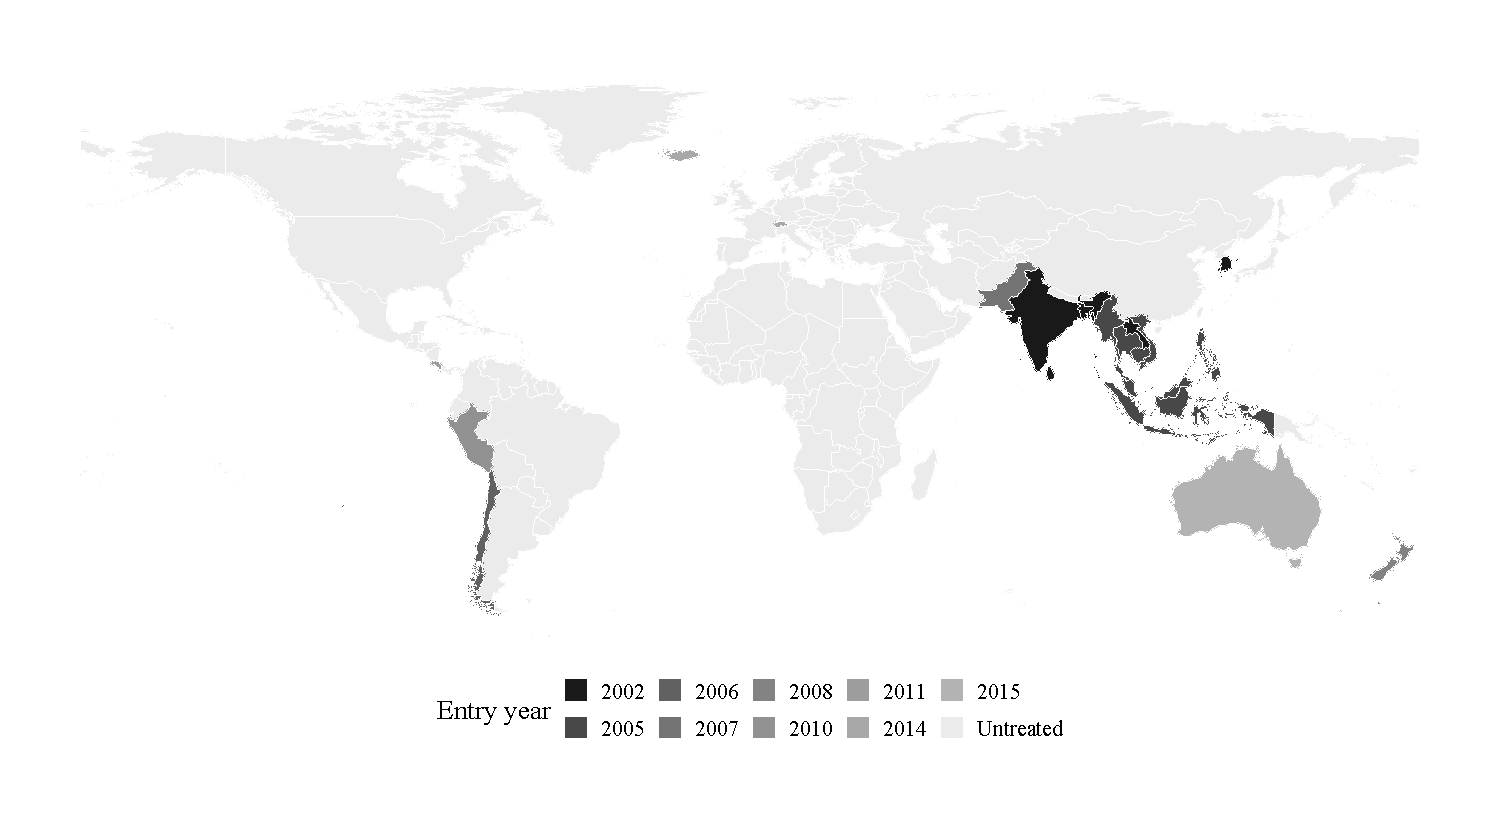
\includegraphics[width=0.85\textwidth]{figures/fig_map_treated.pdf}
\begin{minipage}{0.85\textwidth}\footnotesize
\emph{Notes:} Shaded countries are destinations covered by a Chinese PTA with
environmental provisions during the sample period. Shading indicates the year of entry into
force. Hong Kong and Macao (excluded from the main specification) are not shown. Source: World Bank DTA Database.
\end{minipage}
\end{figure}

\subsection{Customs data and product classification}

The trade data are the universe of Chinese export customs transactions for 2000--2015,
sourced from the Chinese Customs Office. Transactions are aggregated
to the firm--HS6--destination--year level, yielding 49.2 million observations (45.8
million once Hong Kong and Macao are excluded), 462{,}651 exporting firms, 236
destinations, and between 4{,}450 and 4{,}766 HS6 product codes depending on the year. Three outcome variables are used throughout:
the logarithm of export value ($\ln x^{val}_{fpdt}$), the logarithm of export quantity
($\ln x^{qua}_{fpdt}$), and the logarithm of unit value ($\ln x^{uv}_{fpdt}$, defined as
value divided by quantity). Export value is the primary outcome; quantity and unit value serve as decomposition checks.

\emph{Green products} are the 248 HS6 codes of the OECD Combined List of Environmental
Goods (CLEG), as classified in \citet{sauvage2014}. The customs panel uses the HS1996
vintage while the OECD list is defined in HS2012, so the list was harmonized. Of the 248
codes, 246 have a one-to-one mapping to HS1996 and are translated directly. The remaining
two (codes 871411 and 871419, which correspond to a single HS1996 heading split into two
sub-codes in HS2012) are retained at the original HS1996 level; these two codes jointly
account for a negligible share of green-goods trade, so no information of consequence is
lost.
\footnote{As a check on the classification itself, the specification was re-estimated
restricting green products to the 54 codes of the APEC Environmental Goods List
\citep{sauvage2014}, on which there is explicit multilateral political consensus and which
form a complete subset of the OECD list. With the WB index the green coefficient flips
sign to $+0.0050$ (s.e.\ 0.0127, $p=0.69$); with TREND it moves from $+0.0018$ to
$+0.0032$ ($p=0.13$). Both remain indistinguishable from zero, with standard errors
roughly double, as expected from restricting to 22\% of the original green sample. Appendix Table~\ref{tab:apec} reports the full comparison.}

\emph{Dirty products} belong to the classic pollution-intensive sectors of
\citet{mani1998} and \citet{low1992}: pulp and paper, industrial chemicals, petroleum
refining, iron and steel, and non-ferrous metals, with cement added in an extended
variant.\footnote{Products are mapped from ISIC Rev.2 to HS1996 using the official WITS/UNSD concordance, yielding 1{,}139 dirty HS6 codes. Seventeen codes that appear in both lists are assigned to the green category; the two lists are mutually exclusive.}

The remaining HS6 codes form the neutral comparison group. Summary statistics appear in Table~\ref{tab:sumstats}.

\begin{table}[htbp]
\centering
\caption{Summary statistics (full panel, excl.\ HK--MO)}
\label{tab:sumstats}
\small
\begin{threeparttable}
\begin{tabular}{lrrrrr}
\toprule
Variable & N & Mean & Median & Std.\ Dev. & Range \\
\midrule
$\ln x^{val}_{fpdt}$ & 45{,}781{,}181 & 9.264 & 9.360 & 2.546 & [0, 23.3] \\
$\ln x^{qua}_{fpdt}$ & 45{,}470{,}053 & 7.312 & 7.595 & 3.213 & [$-$6.9, 25.7] \\
$\ln x^{uv}_{fpdt}$  & 45{,}470{,}040 & 1.986 & 1.609 & 2.306 & [$-$13.0, 20.4] \\
$g_p$ (green)         & 45{,}781{,}211 & 0.115 & 0 & 0.319 & \{0, 1\} \\
$b_p$ (dirty)         & 45{,}781{,}211 & 0.070 & 0 & 0.255 & \{0, 1\} \\
$EP^{WB}_{dt}$        & 45{,}781{,}211 & 0.966 & 0 & 2.383 & [0, 17] \\
$EP^{TR}_{dt}$        & 45{,}781{,}211 & 2.051 & 0 & 8.165 & [0, 72] \\
$\tau_{pdt}$          & 41{,}117{,}073 & 1.658 & 1.792 & 1.027 & [0, 7.3] \\
$HHI_{pdt}$           & 45{,}306{,}336 & $-$1.540 & $-$1.610 & 0.592 & [$-$3.3, 0] \\
\midrule
\multicolumn{6}{@{}l}{\textit{Collapsed panel}} \\
$\bar{y}_{pdt}$ (collapsed) & 3{,}773{,}498 & 8.974 & 9.029 & 1.957 & [0, 20.7] \\
Cell count $n_{pdt}$        & 3{,}773{,}498 & 12.13 & 3 & 43.64 & [1, 8{,}946] \\
\bottomrule
\end{tabular}
\begin{tablenotes}\footnotesize
\item \emph{Notes:} 45{,}781{,}211 firm--HS6--destination--year observations after excluding Hong Kong
and Macao. Observation counts differ across variables due to missing tariff data and
quantity/unit-value availability. Thirty observations with zero recorded export value have no log
export value. Source: Chinese Customs Office; World Bank DTA Database; TREND Database.
\end{tablenotes}
\end{threeparttable}
\end{table}


Figure~\ref{fig:composition} plots the share of green and dirty products in total export
value over time, separately for treated and untreated destinations. For green products the two
groups track each other closely throughout, with no visible divergence after agreements enter into
force. The dirty share is about twice as high toward treated destinations and rises faster between
2002 and 2008, which reflects the product mix of the early partners (India, ASEAN) rather than a
response to environmental content: the level difference is absorbed by the destination fixed
effects, and the pre-treatment coefficients of the event study (Figure~\ref{fig:es}) are flat.

\begin{figure}[htbp]
\centering
\caption{Green and dirty export shares by treatment status, 2000--2015}
\label{fig:composition}
\vspace{6pt}

\includegraphics[width=0.85\textwidth]{figures/fig_composition_shares.pdf}
\begin{minipage}{0.85\textwidth}\footnotesize
\emph{Notes:} Share of export value accounted for by green and dirty products, computed
separately for destinations with positive EP depth (treated) and destinations with no
PTA or no EP content (untreated) in each year. Excludes Hong Kong and Macao. Source: Chinese Customs Office.
\end{minipage}
\end{figure}

\subsection{Estimation samples}

The analysis rests on four estimation objects built from the same underlying panel; their sizes and fixed-effect structures are summarized in Table~\ref{tab:descriptives}.

\begin{table}[htbp]
\centering
\caption{Descriptive statistics}
\label{tab:descriptives}
\small
\begin{threeparttable}
\begin{tabular}{lr}
\toprule
\multicolumn{2}{l}{\textit{Full firm-level panel (excl.\ HK--MO)}} \\
\midrule
Observations (firm--HS6--dest--year) & 45{,}781{,}211 \\
Exporting firms & 462{,}651 \\
HS6 products & 4{,}450--4{,}766 \\
Destinations & 236 \\
\quad of which treated (EP depth $>0$) & 23 \\
Distinct EP profiles (depth $\times$ timing) & 13 \\
Share of observations: green products & 11.5\% \\
Share of observations: dirty products & 7.0\% \\
Share of observations under an EP agreement & 20.3\% \\
\midrule
\multicolumn{2}{l}{\textit{Collapsed panel (HS6--dest--year)}} \\
\midrule
Cells & 3{,}773{,}498 \\
\quad of which green / dirty & 8.4\% / 14.0\% \\
Estimation sample (post-singleton) & 3{,}681{,}023 \\
\midrule
\multicolumn{2}{l}{\textit{PPML zero-filled grid (HS6--dest--year, excl.\ HK--MO)}} \\
\midrule
Cells & 8{,}179{,}904 \\
\bottomrule
\end{tabular}
\begin{tablenotes}\footnotesize
\item \emph{Notes:} Hong Kong and Macao excluded throughout (they account for 24.4\% of treated
observations and 50.1\% of treated export value). Product classification as described
in the text. Source: Chinese Customs Office.
\item The green and dirty shares differ between the two panels because collapsing changes the unit
of observation from the firm to the cell: green products are exported by more firms per
product--destination cell, so their weight falls from 11.5\% of observations to 8.4\% of cells,
while dirty products have fewer exporting firms per cell and their weight rises from 7.0\% to
14.0\%. The two panels contain the same underlying transactions.
\end{tablenotes}
\end{threeparttable}
\end{table}

The \emph{full firm-level panel} is the main estimation object, with 45.8 million
observations at the firm--HS6--destination--year level. The outcome variables are
$\ln x^{val}_{fpdt}$, $\ln x^{qua}_{fpdt}$, and $\ln x^{uv}_{fpdt}$; the main fixed
effects are firm--product--destination ($\theta_{fpd}$), firm--destination--year
($\theta_{fdt}$), and product--year ($\theta_{pt}$). Standard errors are clustered by
destination.

The \emph{collapsed panel} aggregates the firm dimension, yielding 3.77 million
HS6--destination--year cells. The outcome in each cell is the mean of log exports across
the underlying firm-level observations, and regressions are weighted by the cell count
(the number of firm-level observations in each cell). Fixed effects are
product--destination ($pd$), destination--year ($dt$), and product--year ($pt$). The
collapsed panel serves two purposes: it is a computational workhorse for the bootstrap
and permutation inference battery, and it provides an internal cross-check against the
full panel.\footnote{With 45.8 million observations and three sets of high-dimensional
fixed effects, the full panel is computationally intensive, and the bootstrap requires
several hours per specification. The collapsed panel reduces dimensionality by a
factor of twelve, making the full inference battery feasible on a single machine. The
equivalence between the two implementations is verified algebraically and numerically
in Appendix~\ref{app:pddt}.} The two panels agree on the green margin; Section~\ref{sec:collapsed} explains why they diverge on the dirty margin.

The \emph{zero-filled PPML grid} (8.2 million cells) is built from the full panel by
first aggregating to HS6--destination--year cells and then adding product--destination
pairs with no recorded trade in a given year, conditional on the pair having at least one
positive flow elsewhere in the sample period.\footnote{This conditional zero-fill --- rather than a
complete cross-join of all products, destinations, and years --- keeps the grid
computationally tractable while capturing the relevant extensive margin. A zero-fill at the firm--product--destination--year level would generate
billions of rows, making estimation computationally infeasible; a PPML without zero-fill would miss the
extensive margin entirely, since the estimator's advantage lies precisely in the
information contained in the zeros.}

Because the triple-difference compares green and dirty products to neutral ones, the
credibility of the comparison group can be probed directly. Four control-group subsamples,
each tightening the comparison in the direction of a specific threat, are summarized in
Table~\ref{tab:samples} and described below. The prefix C- denotes the control-group variant.

\begin{table}[htbp]
\centering
\caption{Control-group subsamples}
\label{tab:samples}
\small
\begin{threeparttable}
\begin{tabular}{@{}p{4.4cm}p{5.4cm}r@{}}
\toprule
Subsample & Threat addressed & Obs. \\
\midrule
\textbf{C-prod-HS4}\newline \emph{\small neutral products in the same HS4 family as a green code} & Neutral products differ from green and dirty ones & 3.8M \\
\addlinespace
\textbf{CEM destinations}\newline \emph{\small destinations matched on year-2000 GDP p.c., growth, MFN tariff} & Selection of partner countries & 14.0M \\
\addlinespace
\textbf{Deep vs.\ shallow}\newline \emph{\small PTA partners only, split at median EP depth} & The ``any-agreement'' contrast itself & 5.3M \\
\bottomrule
\end{tabular}
\begin{tablenotes}\footnotesize
\item \emph{Notes:} All observation counts refer to the full firm-level panel (excl.\ HK--MO). Source: Chinese Customs Office; World Bank DTA Database; TREND Database.
\end{tablenotes}
\end{threeparttable}
\end{table}

\emph{C-prod-HS4} restricts the neutral comparison group to products belonging to the
same HS4 family as a green code (106 HS4 families, covering 20.5\% of observations).
This guards against the concern that neutral products are too dissimilar from green ones
to serve as a valid counterfactual. It should be read alongside C-overlap: multi-product
firms may reallocate toward core products when trade costs fall \citep{eckel2010},
potentially displacing neutral products in the same HS4 family and biasing the contrast.

\emph{C-overlap} retains only products exported to both treated and untreated destinations (98.5\% of all HS6 codes, 21.5 million observations). This ensures that the identifying variation does not rely on products traded exclusively with one group of destinations, guarding against the possibility that multi-product firms reallocate across products within the same HS4 family when trade costs fall \citep{eckel2010}.\footnote{In practice the restriction is close to non-binding: it removes 314 of the 21{,}519{,}511 observations in the estimation sample, and the estimates it produces are indistinguishable from the baseline to the fourth decimal. For that reason it is reported in the robustness battery of Appendix~\ref{app:robustfull} rather than alongside the three subsamples that genuinely change the comparison group in Section~\ref{sec:comparison}.}

\emph{CEM destinations} applies coarsened exact matching \citep{iacus2012} at the
destination level, matching treated destinations to untreated ones on year-2000 GDP per
capita, GDP growth, and MFN tariff levels. The multivariate $L_1$ imbalance falls from
0.68 before matching to 0.43 on the matched sample. The resulting sample contains 19 treated and
40 control destinations (13,992,396 observations after iterative singleton removal) and addresses the concern that
treated and untreated destinations differ systematically on dimensions correlated with
export composition.

\emph{Deep vs.\ shallow} drops all untreated destinations and splits the remaining PTA
partners at the median EP depth (median computed over the 25 PTA partners including Hong Kong and Macao; 16 deep and 9 shallow, of which 16 and 7 remain in the baseline sample; 5.3 million
observations). This design asks whether composition differs between deep and shallow
environmental chapters, conditional on having an agreement at all, and addresses the
concern that any observed effect reflects the agreement rather than its environmental
content.

A genuine composition effect should survive every change to the comparison group; an artifact will move when the comparison changes.

% ============================================================================
\section{Empirical Strategy}\label{sec:strategy}
% ============================================================================

Three challenges shape the identification strategy: countries select into agreements, environmental and overall agreement depth correlate strongly, and the number of independent treatment units is small.

A starting point would be to estimate the level effect of environmental provisions
on trade---regressing log exports on environmental depth with fixed effects. A
structural argument shows why this is uninformative in this setting.

The argument is independent of the empirical results. Any fixed-effects
structure that seriously addresses bilateral confounders requires a destination--year
intercept, which absorbs \emph{all} variation at the $(d,t)$ level---including
environmental depth itself. With only 13 distinct EP profiles and
near-zero within-destination change over time, ``environmental depth'' and ``having a
deep agreement'' are empirically indistinguishable. The interaction
$EP_{dt} \times g_p$ survives the destination--year intercept because the product
dimension varies \emph{within} the $(d,t)$ cell. This is why the specification is
built on composition---the differential response of green and dirty products relative
to neutral ones---rather than on levels.

This design cannot show that EP-heavy agreements affected aggregate trade levels --- that effect is confounded with the agreement itself. The evidence speaks only to the composition margin.

\subsection{The triple-difference specification}

The question is whether environmental depth shifts the gap between green (or dirty)
and neutral log exports among treated
destinations.\footnote{In potential-outcomes terms, the target can be written as
$\beta_1 = E\bigl[(y_{fpgdt}(1)-y_{fpgdt}(0)) - (y_{fpndt}(1)-y_{fpndt}(0))
\mid d,t \text{ treated}\bigr]$, where $y(1)$ and $y(0)$ denote log exports of
green product $g$ versus neutral product $n$ under deeper and unchanged environmental
content respectively, holding the agreement fixed.}
OLS gives equal weight to each observation, so the coefficient is a
per-observation average, not a per-firm or per-destination average.\footnote{A firm exporting 100 products receives 100 times the weight of a firm exporting one product. The coefficient therefore reflects the composition of the estimation sample rather than a simple average across firms or destinations.} The main
specification is
\begin{equation}\label{eq:main}
\ln x_{fpdt} = \beta_1\, EP_{dt}\!\times\!g_p + \beta_2\, EP_{dt}\!\times\!b_p
+ \gamma_1\, TD_{dt}\!\times\!g_p + \gamma_2\, TD_{dt}\!\times\!b_p
+ \theta_{fpd} + \theta_{fdt} + \theta_{pt} + \varepsilon_{fpdt},
\end{equation}
where $f$ indexes firms, $p$ HS6 products, $d$ destinations, and $t$ years; $g_p$
and $b_p$ are the green and dirty product indicators defined in
Section~\ref{sec:background}; $EP_{dt}$ is environmental depth and $TD_{dt}$
non-environmental agreement depth. Environmental depth enters the regression only
through its interactions with $g_p$ and $b_p$, not on its own: the level effect of
$EP_{dt}$ is absorbed by $\theta_{fdt}$, and what remains is the differential
response of green and dirty products relative to neutral ones.

The three sets of fixed effects absorb different sources of confounding variation,
and the choice of which to include is dictated by the structure of the treatment.

The firm--product--destination fixed effects $\theta_{fpd}$ absorb time-invariant
features of each firm--product--market relationship---for example, a firm's
long-standing contract with a South Korean buyer of solar panels, or an established
network for exporting steel to a particular ASEAN destination.

The firm--destination--year fixed effects $\theta_{fdt}$ are what drives
identification. They absorb all time-varying bilateral factors --- entry into new markets, aggregate demand shifts, exchange rate movements --- that affect a firm's exports to a destination uniformly across products. The agreement dummy, overall agreement depth, destination demand shocks, and the non-random selection of destinations into agreements all drop out. Identification comes from comparing green and dirty products to neutral ones \emph{within} the same cell as environmental content varies across destinations and over time.

The product--year fixed effects $\theta_{pt}$ absorb global product-level shocks
common to all destinations---for instance, the worldwide expansion of the solar
panel market in the late 2000s, or global fluctuations in steel prices---so that
these shocks do not contaminate the composition comparison.\footnote{Firm--product--year fixed effects would be computationally infeasible given the panel size. Product--year effects are sufficient because firm--product shocks that do not vary across destinations are already absorbed by the combination of $\theta_{fpd}$ and $\theta_{fdt}$.}

The three-way fixed-effect structure absorbs a large number of singletons
--- observations whose identifying variation is fully accounted for by at
least one fixed effect.  Iterative singleton removal
\citep{correia2017} reduces the estimation sample from 45.8 million
raw observations to 21,519,511 in the full panel (a 53\% reduction)
and from 3,773,498 cells to 3,681,023 in the collapsed panel.

Selection into agreements is not eliminated but substantially narrowed: $\theta_{fdt}$ absorbs the level effect, so selection contaminates $\beta_1$ only through differential pre-trends in green versus neutral exports across destinations. Appendix~\ref{app:trends} tests this directly with destination-specific trends and finds no change in the green coefficient.

The omitted category is neutral products. $\beta_1$ measures how green products
move \emph{relative to neutral ones} as environmental depth increases; $\beta_2$
measures the same contrast for dirty products. Each coefficient is already the
difference from the neutral baseline. The green--dirty differential
($\beta_1 - \beta_2$) is a derived quantity, not the parameter the regression
identifies, and should not be read as such.

The same World Bank non-environmental depth control is used in both the WB and the TREND specifications: TREND does not code non-environmental provisions, so no TREND-based analogue exists.

The non-environmental depth interactions ($TD_{dt} \times g_p$ and
$TD_{dt} \times b_p$) separate environmental from general agreement content.
$TD_{dt}$ counts all non-environmental provisions, but not all of these are
directly relevant to green or dirty trade; it is therefore an imperfect proxy for
the non-environmental component of agreement depth that might independently affect
export composition. An imperfectly measured control under-controls: $\beta_1$
absorbs whatever share of general-depth variation the proxy fails to
capture.\footnote{If the non-environmental depth control imperfectly measures the true confounding depth, $\hat{\beta}_1$ absorbs the part of general-depth variation the proxy misses. Because EP and total depth correlate at $\rho = 0.91$, this omitted component is positively associated with EP, so the bias pushes $\hat{\beta}_1$ upward. With a null green coefficient, any upward bias implies the true effect is zero or negative --- the null is a conservative reading of the data.} Rather than assert a direction, Appendix~\ref{app:depthbounds} reports the
green coefficient under four alternative depth controls and shows that the point
estimate moves within a band narrower than one standard error
(Table~\ref{tab:depthbounds}).

Collinearity between EP depth and non-environmental depth is substantial: the two correlate at $\rho = 0.91$ across treated destination--years --- and more tightly still once the fixed effects are partialled out, as Section~\ref{sec:fullpanel} shows --- and the variance inflation factor of EP depth regressed on non-environmental depth across treated destination--years is 5.8.\footnote{The Variance Inflation Factor measures how much collinearity inflates the variance of the estimated coefficient relative to an orthogonal design. Here it is computed on the two depth variables at the destination--year level, not on the interacted regressors of the estimating equation. A VIF of 5.8 is somewhat above the maximum of 4.6 that \citet{brandi2020} report for their provision-type variables on a panel of 680 agreements.}
The TREND count is less
collinear with non-environmental depth ($\rho = 0.50$), which is one reason the WB
confidence intervals are wider. That two codings with such different degrees of
overlap return the same null is reassuring, since a result driven by the inability
to separate environmental from general depth would be expected to differ between
them.

Standard errors are clustered by destination. EP depth varies across destinations and years but changes in only three destinations during the sample period, making treatment effectively destination-level. Clustering by destination treats all observations from the same country as a single cluster, which is the appropriate level when the treatment is in practice a destination-level assignment \citep{abadie2023}.

A further identification concern works in a conservative direction. If deeper
environmental chapters tend to be signed where green demand is already rising,
$EP_{dt}$ is positively correlated with an omitted destination-specific trend,
which would bias $\beta_1$ positively. With a null coefficient, any upward bias from this channel implies the true effect is zero or negative---the null is a conservative rather than a lenient reading of the data.

Because environmental depth is a continuous dose switching on at staggered dates,
the coefficient is a weighted average of dose- and cohort-specific composition
responses, not a simple average treatment effect. For the green margin the dose-specific estimates of Appendix~\ref{app:dose} are all close to zero, so the weighting is immaterial; for the dirty margin they are not, and the linear coefficient should be read as a summary of a contrast between the medium-depth ASEAN cohort and the rest rather than as a per-provision slope.\footnote{Under continuous treatment entering at
staggered dates, the TWFE estimator produces a weighted average of dose- and
cohort-specific effects whose weights need not be convex
\citep{callaway2024, goodmanbacon2021, dechaisemartin2020}. Two features limit
what this costs in this setting. First, a weighted average of near-zero effects
stays near zero unless the underlying effects are large and of opposite signs, of
which the sub-index and leave-one-out evidence gives no indication. Second, the
permutation test is agnostic about weighting: it asks whether the observed
coefficient---whatever weighted average it represents---is unusual relative to
placebos.}

\subsection{Inference with few treated clusters}\label{sec:inference}

Of the destination clusters in the estimation sample, only 23 are treated,
corresponding to 13 distinct EP profiles. With so few treated
clusters, asymptotic cluster-robust standard errors are unreliable: the
finite-sample approximation to the $t$-distribution is too optimistic, and
$p$-values systematically over-reject the null
\citep{cameron2008, mackinnon2017}. Every headline estimate is therefore subjected
to two additional tests.

\emph{Wild cluster bootstrap.}
The wild cluster bootstrap \citep{cameron2008, roodman2019} provides inference that does not rely on asymptotic critical values and is appropriate for settings with few clusters. In both panels, fixed effects are partialled out via the Frisch--Waugh theorem before the bootstrap is applied, because the bootstrap implementation requires a single set of absorbed effects. Point estimates are identical to those from the direct estimation; only computational cost differs.\footnote{Partialling out introduces two minor approximations. First, the bootstrap treats all fixed effects as if nested within the destination cluster. In the full panel this is nearly true: firm--product--destination and firm--destination--year are each nested within a destination; only product--year is not. In the collapsed panel the nesting is less complete (only destination--year is strictly nested), so the approximation is somewhat less tight. Second, the small-sample adjustment sees only the residualized regressors rather than the regressors plus the absorbed fixed effects. Neither approximation has practical relevance here: the conclusions are insensitive to the choice of panel, and the collapsed-panel dirty coefficient has a bootstrap $p$-value of 0.07 and the full-panel one of 0.19 regardless of which approximation applies.}

\emph{Permutation inference.}
The permutation test reshuffles EP profiles across the 23 treated destinations, testing whether the specific EP content --- not the agreement itself --- matters for composition.\footnote{The test operates only among treated destinations because permuting between treated and untreated destinations would test a different hypothesis (the effect of the agreement as such), which is unidentifiable as shown in Section~\ref{sec:strategy}.} With $1{,}000$ replications, the test asks whether the observed coefficient is unusual relative to the placebo distribution.

Because depth and timing are permuted jointly, the test cannot separate the effect
of environmental content from the effect of entry timing. The whole time path of each profile moves with it, including entry timing and the non-environmental depth control, so the null hypothesis is that, given the set of destinations that ever sign, it does not matter which of them received which profile.\footnote{Estimates on the collapsed and destination-level panels were produced twice, in \textsc{Stata}
(\texttt{reghdfe}, \citealp{correia2017}; \texttt{boottest},
\citealp{roodman2019}; \texttt{ppmlhdfe}, \citealp{correia2020};
\texttt{eventstudyinteract}, \citealp{sun2021}) and in \textsc{R}
(\texttt{fixest}, \texttt{fwildclusterboot}); across 44 result files the two implementations agree on every point estimate to at least
seven significant digits. Estimates on the 45.8-million-row firm-level panel exist only in \textsc{Stata}: \texttt{fixest} cannot complete them on the available hardware. They are validated instead by an algebraic identity---the firm-level panel estimated with $pd+dt+pt$ fixed effects reproduces the weighted collapsed-panel estimate to nine significant digits (Appendix~\ref{app:pddt})---which checks the data construction of the two pipelines against each other. All reported numbers are the \textsc{Stata}
ones. Two quantities
legitimately differ between implementations and are discussed where they arise:
bootstrap and permutation $p$-values, which carry Monte Carlo error, and the
Sun--Abraham standard errors of Appendix~\ref{app:sunab}, which reflect a genuine
methodological difference between \texttt{eventstudyinteract} and
\texttt{fixest::sunab} (see Appendix~\ref{app:sunab}).}

Bootstrap and permutation $p$-values accompany every estimate in Section~\ref{sec:results}; the
complete set, across both panels, both indices and all four sample--depth variants, is collected in
Appendix~\ref{app:inference} (Tables~\ref{tab:wcb} and~\ref{tab:perm}).
% ============================================================================
\section{Results}\label{sec:results}
% ============================================================================

\subsection{Fixed effects and the reference specification}\label{sec:fe}

Before reading a single coefficient it is worth establishing that the fixed-effect structure of
equation~\eqref{eq:main} earns its cost. Table~\ref{tab:ladder_compact} estimates the same
composition interactions on the same panel under five sets of absorbed effects, moving from the
sparsest to the specification used in the rest of this section. The dependent variable is log export
value throughout, so the columns differ only in what they hold fixed.

The first four columns tell a coherent and misleading story. The World Bank dirty interaction is
positive and significant at $+0.0064$ in column~(4), and the TREND green interaction is positive and
significant at $+0.0018$ in the same column; in column~(3) both are again positive and significant
at the ten percent level or better. Read on their own, these say that agreements with deeper environmental chapters
saw both green and dirty exports grow relative to neutral ones --- which is not a composition effect
at all, since the two ends move the same way.

What the four columns have in common is the explanation. None of them contains a fixed effect with
both a destination and a time dimension. Chinese exports to a partner grow around the entry into
force of an agreement for reasons that have nothing to do with its environmental chapter: tariffs
fall, the partner's income rises, the trading relationship deepens. That growth is a
destination--time phenomenon, and with no destination--time absorber it has nowhere to go except onto
whichever interaction is correlated with agreement timing --- which is exactly what the EP
interactions are, since the destinations with environmental content are the destinations with
agreements.

Column~(5) adds firm--destination--year effects and the picture changes completely. The World Bank
dirty coefficient goes from $+0.0064$ to $-0.0044$, the TREND green coefficient from $+0.0018$ to
$-0.0001$, and the significance disappears with the sign. We cannot say which destination-specific
shock was driving the earlier columns, only that it had a destination--time structure, because
absorbing that structure is what removes it. This is the empirical counterpart to the argument made
on structural grounds in Section~\ref{sec:strategy}, and it is why the saturated specification is not
one defensible choice among five but the only one in the sequence that removes a confounder visible
in the data.

Column~(5) is the specification of Table~\ref{tab:fullpanel} and of everything that follows.
Appendix~\ref{app:ladder} reports the same ladder for quantity and unit value, where the pattern
repeats.

\input{Tabelle/tab_01_ladder}

\FloatBarrier
\subsection{The full panel}\label{sec:fullpanel}

Table~\ref{tab:fullpanel} reports the estimates on the full firm--product--destination--year panel.
There are twelve coefficients of interest in it, and they are easier to read across than down.
Columns~(1)--(3) measure environmental content with the World Bank depth index and columns~(4)--(6)
with the TREND provision count; within each block the outcome is log export value, then log quantity,
then log unit value. Panel~A controls for non-environmental World Bank depth and Panel~B for the
independently coded DESTA index \citep{dur2014}. The green and dirty interactions are estimated
jointly and should be read together: the design asks whether an environmental chapter tilts a firm's
product mix, and a tilt has two ends.

Only one of those ends moves. On the green margin the coefficient is indistinguishable from zero in
every cell. Export value gives $-0.0023$ (s.e.\ 0.0039) with the World Bank index and $-0.0001$
(0.0010) with TREND; switching the depth control to DESTA changes the third decimal and nothing else.
The joint $F$-test on all four composition interactions returns $p = 0.31$ (WB) and $p = 0.71$ (TREND)
in Panel~A, and $p = 0.18$ and $p = 0.26$ in Panel~B. Quantity and unit value add nothing: across the
eight green cells in columns~(2), (3), (5) and~(6) no coefficient comes close to significance. That
rules out the one reading a value regression alone cannot dismiss --- that a volume response and a
price response are offsetting each other inside the value aggregate. Neither channel moves. If
Chinese firms shifted toward environmental goods when an agreement with environmental content entered
into force, the shift is not visible here at any margin.

The dirty coefficient does move, and it is worth being precise about how much. In Panel~A it is
$-0.0044$ on export value with an asymptotic $p$-value of 0.052, and $-0.0009$ with $p = 0.15$ under
TREND. In Panel~B the same two coefficients are $-0.0056$ ($p = 0.039$) and $-0.0014$ ($p = 0.048$).
The sign is stable, the magnitude is stable, and the asymptotic verdict depends on which measure of
non-environmental agreement depth sits in the regression. That dependence has a mechanical
explanation. Within destinations and years, environmental depth correlates $0.959$ with World Bank
non-environmental depth and $0.891$ with DESTA depth.\footnote{Correlations of the two depth
measures after removing destination and year means, computed on the treated destination--years
(223 with the World Bank control, 212 with DESTA, which does not cover Timor-Leste). They are
higher than the raw correlation of $\rho = 0.91$ because the demeaning removes the variation the
two measures share across destinations. They are a property of the treatment variables, not of the
interacted regressors of equation~\eqref{eq:main}.} The World
Bank control absorbs almost the same variation as the regressor of interest, so little independent
variation is left and the standard error is wide; DESTA overlaps less, leaves more, and the standard
error narrows. Nothing about the estimated effect changes between the panels --- only how much of it
the design can see.

This is the point at which asymptotic $p$-values stop being informative, for the reasons set out in
Section~\ref{sec:inference}: with 23 treated destinations and 13 distinct agreement profiles,
cluster-robust inference over-rejects. The row labelled ``Bootstrap $p$'' in this and every subsequent
table reports the wild cluster bootstrap with $B = 9{,}999$ replications, and it is the reference
inference throughout. The asymptotic figures are kept alongside it only so that the gap between the
two remains visible.

The gap is large exactly where it matters. On the green margin the bootstrap changes nothing: $p$
moves from 0.57 to 0.69 (WB) and from 0.92 to 0.93 (TREND), and the null is a null either way. On the
dirty margin under the World Bank control it changes the verdict, taking $p$ from 0.052 to 0.19 and
from 0.15 to 0.18. Under DESTA it does not: 0.039 becomes 0.049 and 0.048 becomes 0.069. So the dirty
coefficient survives robust inference under one depth control and not under the other, and it does so
on both codings at once, which at least means the two databases are telling the same story. The place
where it is strongest is quantity: under DESTA the World Bank interaction is $-0.0070$ on log quantity
with a bootstrap $p$ of 0.035, larger and better determined than on value, while the unit value
coefficient is $+0.0004$ and nowhere near significance. Whatever this is, it is a shipment volume and
not a price. Section~\ref{sec:collapsed} brings to bear the one test that does not depend on the
choice of depth control.

The sign, at least, is where the recent literature on China would put it. \citet{yue2024} find that
environmental provisions in China's PTAs inhibit exports of energy-consuming products, and
\citet{zhusun2026}, working with customs data that overlap with those used here, report that
environmental provisions reduce dirty exports and raise green ones. On dirty the present estimates
agree in sign and are considerably smaller; on green they do not agree at all. The difference is not
mysterious, and Section~\ref{sec:collapsed} measures it: their identification comes from variation
across firms and destinations, which is precisely the variation that $\theta_{fdt}$ removes here.
\citet{zhusun2025} report that environmental provisions are associated with quality upgrading in
Chinese firms' exports; unit value is a coarse proxy for quality and column~(3) is null, but the
outcome and the sample differ enough that this should not be read as a test of their result.

A null is only as informative as the interval around it. The 95\% wild cluster bootstrap confidence
interval for the green interaction runs from $-0.0353$ to $+0.0355$ per World Bank provision, roughly
$\pm 3.5$ percent. Since one standard deviation of World Bank EP depth in the estimation sample is
about 2.4 provisions, that bound implies at most an eight to nine percent change in green relative to
neutral exports for a one-standard-deviation increase in environmental content. Stated per agreement rather than per provision, the bound is looser: for the six provisions of the
ASEAN chapter it is about $\pm 21$ percent, and for the sixteen-provision jump of the Korea agreement
it exceeds $\pm 40$ percent. The null is bounded at the provision level, not at the level of a deep
agreement. The corresponding
asymptotic interval, $[-0.0100, +0.0055]$, is roughly four and a half times narrower; reporting that width would
claim a precision Section~\ref{sec:inference} has already declared unwarranted. The statement this
paper can defend is therefore not ``there is no effect'' but ``any effect is smaller than about three
percent per provision'', which is a bound, not an absence. Appendix Table~\ref{tab:mde} reports the
corresponding minimum detectable effects on the collapsed panel, where the standard errors are larger
and the bounds correspondingly looser.

\begin{table}[htbp]
\centering
\footnotesize
\caption{Full panel --- triple-difference estimates}
\label{tab:fullpanel}
\begin{threeparttable}
\begin{tabular}{lcccccc}
\toprule
 & \multicolumn{3}{c}{WB EP depth ($EP^{WB}_{dt}$)} & \multicolumn{3}{c}{TREND EP count ($EP^{TR}_{dt}$)} \\
\cmidrule(lr){2-4}\cmidrule(lr){5-7}
 & (1) & (2) & (3) & (4) & (5) & (6) \\
 & $\ln x^{val}_{fpdt}$ & $\ln x^{qua}_{fpdt}$ & $\ln x^{uv}_{fpdt}$ & $\ln x^{val}_{fpdt}$ & $\ln x^{qua}_{fpdt}$ & $\ln x^{uv}_{fpdt}$ \\
\midrule
\multicolumn{7}{l}{\textit{Panel A --- Non-environmental depth control ($TD_{dt}$, World Bank)}} \\[3pt]
$EP_{dt} \times g_p$ & $-$0.0023 & $-$0.0013 & $-$0.0004 & $-$0.0001 & $-$0.00003 & $-$0.0001 \\
 & (0.0039) & (0.0041) & (0.0013) & (0.0010) & (0.0011) & (0.0003) \\[2pt]
\quad Asymptotic $p$ & [0.566] & [0.750] & [0.748] & [0.924] & [0.974] & [0.857] \\
\quad Bootstrap $p$ & [0.686] & [0.851] & [0.740] & [0.931] & [0.978] & [0.860] \\[6pt]
$EP_{dt} \times b_p$ & $-$0.0044* & $-$0.0048* & 0.0001 & $-$0.0009 & $-$0.0006 & $-$0.0001 \\
 & (0.0022) & (0.0029) & (0.0010) & (0.0006) & (0.0007) & (0.0004) \\[2pt]
\quad Asymptotic $p$ & [0.052] & [0.096] & [0.903] & [0.153] & [0.409] & [0.697] \\
\quad Bootstrap $p$ & [0.185] & [0.391] & [0.937] & [0.177] & [0.443] & [0.734] \\[6pt]
\quad $\theta_{fpd}$ & \checkmark & \checkmark & \checkmark & \checkmark & \checkmark & \checkmark \\
\quad $\theta_{fdt}$ & \checkmark & \checkmark & \checkmark & \checkmark & \checkmark & \checkmark \\
\quad $\theta_{pt}$ & \checkmark & \checkmark & \checkmark & \checkmark & \checkmark & \checkmark \\
\addlinespace[3pt]
Observations & 21,519,511 & 21,313,047 & 21,313,037 & 21,519,511 & 21,313,047 & 21,313,037 \\
Clusters ($d$) & 225 & 225 & 225 & 225 & 225 & 225 \\
$R^2$ & 0.873 & 0.913 & 0.963 & 0.873 & 0.913 & 0.963 \\
\addlinespace[6pt]
\midrule
\multicolumn{7}{l}{\textit{Panel B --- DESTA depth control}} \\[3pt]
$EP_{dt} \times g_p$ & $-$0.0019 & $-$0.0015 & $-$0.0004 & $-$0.0001 & $-$0.0001 & $-$0.0001 \\
 & (0.0037) & (0.0034) & (0.0019) & (0.0010) & (0.0010) & (0.0005) \\[2pt]
\quad Asymptotic $p$ & [0.613] & [0.660] & [0.819] & [0.904] & [0.917] & [0.776] \\
\quad Bootstrap $p$ & [0.673] & [0.755] & [0.843] & [0.920] & [0.933] & [0.852] \\[6pt]
$EP_{dt} \times b_p$ & $-$0.0056** & $-$0.0070** & 0.0004 & $-$0.0014** & $-$0.0014* & $-$0.00004 \\
 & (0.0027) & (0.0030) & (0.0011) & (0.0007) & (0.0008) & (0.0003) \\[2pt]
\quad Asymptotic $p$ & [0.039] & [0.020] & [0.676] & [0.048] & [0.080] & [0.903] \\
\quad Bootstrap $p$ & [0.049] & [0.035] & [0.765] & [0.069] & [0.100] & [0.915] \\[6pt]
\quad $\theta_{fpd}$ & \checkmark & \checkmark & \checkmark & \checkmark & \checkmark & \checkmark \\
\quad $\theta_{fdt}$ & \checkmark & \checkmark & \checkmark & \checkmark & \checkmark & \checkmark \\
\quad $\theta_{pt}$ & \checkmark & \checkmark & \checkmark & \checkmark & \checkmark & \checkmark \\
\addlinespace[3pt]
Observations & 21,517,666 & 21,311,206 & 21,311,196 & 21,517,666 & 21,311,206 & 21,311,196 \\
Clusters ($d$) & 225 & 225 & 225 & 225 & 225 & 225 \\
$R^2$ & 0.873 & 0.913 & 0.963 & 0.873 & 0.913 & 0.963 \\
\bottomrule
\end{tabular}
\begin{tablenotes}[flushleft]\footnotesize
\item \textit{Notes:} Full firm-level panel, excluding Hong Kong and Macao. Columns~(1) and~(4): log export value ($\ln x^{val}_{fpdt}$). Columns~(2) and~(5): log export quantity ($\ln x^{qua}_{fpdt}$). Columns~(3) and~(6): log unit value ($\ln x^{uv}_{fpdt} = \ln x^{val}_{fpdt} - \ln x^{qua}_{fpdt}$). Quantity and unit-value regressions are estimated on the subset of observations with non-missing quantity data. All specifications include $TD_{dt} \times g_p$ and $TD_{dt} \times b_p$ controls (not shown). Panel~A uses non-environmental WB depth ($TD_{dt}$); Panel~B uses DESTA depth. Standard errors clustered at the destination level in parentheses. Wild cluster bootstrap ($B = 9{,}999$) $p$-values in brackets. $^{*}$~$p<0.10$, $^{**}$~$p<0.05$, $^{***}$~$p<0.01$ (asymptotic).
\item \textit{Source:} Chinese Customs Office; World Bank DTA Database; TREND Database.
\end{tablenotes}
\end{threeparttable}
\end{table}


\FloatBarrier
\subsection{The collapsed panel, and what survives robust inference}\label{sec:collapsed}

Table~\ref{tab:collapsed} repeats the exercise on HS6--destination--year cells weighted by cell size.
Three things change at once and it is worth naming them before reading the numbers. The unit of
observation is a product--destination--year cell rather than a firm--product--destination--year
shipment; the dependent variable is therefore a cell mean of log exports rather than an individual
flow; and the fixed effects become $\theta_{pd} + \theta_{dt} + \theta_{pt}$, since firm identifiers
no longer exist in the collapsed data. The last of these is the substantive change. The firm
dimension of the absorbers is gone, so a shift in \emph{which} firms ship dirty goods to a
destination now enters the coefficient, where in Table~\ref{tab:fullpanel} it was absorbed. The
collapsed panel is not a robustness check on the full panel: it estimates a wider object, and the
difference between the two is informative in its own right.\footnote{The two are related by an exact
algebraic identity when the fixed effects are held the same. Estimating the firm-level panel under
$pd + dt + pt$ reproduces the weighted collapsed-panel coefficient to nine significant digits, which
is what makes the comparison in this section a comparison of fixed-effect structures rather than of
datasets (Appendix~\ref{app:pddt}).}

On green the two panels agree, as they have agreed everywhere so far: $-0.0046$ (bootstrap
$p = 0.65$) with the World Bank index, $+0.0018$ ($p = 0.39$) with TREND, and again nothing on
quantity or unit value. On dirty they do not. The World Bank interaction is $-0.0119$ against
$-0.0044$ in the full panel, a factor of 2.7, with an asymptotic $p$-value below 0.001. Since the two
specifications differ by exactly the between-firm channel, the gap measures it:
$(0.0119 - 0.0044)/0.0119 = 0.63$, so roughly three-fifths of the aggregate dirty association is a
change in the composition of exporters rather than reallocation inside a given firm. This is the
quantity that reconciles the present result with \citet{zhusun2026}. Their design keeps that channel;
equation~\eqref{eq:main} removes it. Neither is wrong, and the two sets of results are not in conflict
once the estimands are stated.

The collapsed panel is also where the design can be attacked with a third test. The wild cluster
bootstrap already raises the dirty $p$-value from below 0.001 to 0.072, which is a large correction,
but the bootstrap still takes the assignment of treatment as given and resamples only the residuals.
The permutation test asks a blunter question. The environmental profile of each agreement --- its
depth and the years in which it takes effect --- is detached from its destination and reassigned at
random among the 23 treated destinations; the model is re-estimated; and the exercise is repeated a
thousand times. The reported $p$-value is the share of these reassignments that produce a coefficient
at least as large in absolute value as the observed one.
The placebo distribution is not centred at zero (its mean is $+0.003$ for the dirty interaction),
so the two-sided figure adds a right tail the alternative does not concern; the one-sided share of
reassignments at least as negative as the observed coefficient is 0.08, and 0.17 after centring on
the placebo mean.
It is computationally expensive, which is
why it is run on export value only, and it is discrete, because thirteen distinct profiles do not
generate a smooth distribution. But it answers the question a reader of this table actually has:
would this number have appeared if we had simply relabelled which of these destinations signed
environmental chapters?

For the dirty coefficient the answer is that it would, 27.8 percent of the time, or 8.1 percent counting only reassignments as negative as the estimate. For green it is 59.7
percent. Under the DESTA control the two figures are 14.6 and 48.0 percent. This settles the question
Section~\ref{sec:fullpanel} could not, because the permutation distribution is built by reassigning whole
agreement profiles rather than by partialling out a control, and it returns the same verdict under
both depth measures (0.28 and 0.15). Appendix Table~\ref{tab:matrice} makes the point from the other direction, assembling
the dirty coefficient across all four sample--depth variants under a single inference method: the
point estimate is uniformly negative, and the bootstrap $p$-value tracks the control variable rather
than the data.

A leave-one-out exercise closes the argument, and it does not close it the way the phrase ``driven by
one country'' usually implies. Table~\ref{tab:loo_new} re-estimates the dirty interaction dropping
each treated destination in turn. The point estimate is remarkably stable: it sits between $-0.0097$
and $-0.0133$ in all 23 samples, and dropping large partners such as India or Pakistan moves it by
one to four percent. What is fragile is the precision. Dropping Australia moves the coefficient by 13
percent, to $-0.0103$, while nearly tripling its standard error from 0.0030 to 0.0087; dropping Korea
doubles the standard error and gives $-0.0097$. Australia and Korea are not outliers pulling the
estimate --- they supply the variation that identifies it --- and both entered into force on 20 December 2015, so the precision of the dirty estimate rests on two destinations observed for eleven days of treatment, and without them the design cannot
determine much of anything. Which of the two is pivotal depends, once again, on the depth control:
under DESTA it is Korea rather than Australia. A coefficient whose decisive observation is selected
by a modelling choice unrelated to environmental content is behaving the way the permutation test
already suggested it was.

The same exercise on the green margin (Table~\ref{tab:loo_green}) is quieter but not featureless.
Dropping Switzerland moves the green coefficient to $-0.011$ (asymptotic $p < 0.001$), the one
leave-one-out sample in which it reaches significance; dropping Korea or Australia moves it to
$+0.003$ and $+0.002$, with standard errors roughly 1.5 and 1.9 times the baseline. The point
estimate stays inside a narrow band for every other destination, but its precision, like the dirty
coefficient's, is not uniform across the sample.

One ambiguity we do not resolve. Australia and Korea are also the destinations with the deepest
environmental coverage in the sample, so a dose--response reading --- the effect is real and
concentrated where the dose is largest --- is not ruled out by the leave-one-out geometry alone.
Taken together with the permutation result, however, the reading we adopt is that the dirty
association is present in the data but cannot be distinguished from what random relabelling of the
same destinations produces.

A second consideration cuts the other way. The under-control argument of Section~\ref{sec:strategy}
--- an imperfect depth control lets $EP_{dt}$ absorb part of the effect of general agreement depth
--- biases both interactions upward. For the green margin this makes the null conservative; for the
dirty margin it implies that the true coefficient is, if anything, more negative than the estimate.
We note this rather than resolve it: the permutation test, which reassigns environmental and
non-environmental content together, is unaffected by the quality of the control, and it is the test
on which the reading above rests.

\begin{table}[htbp]
\centering
\footnotesize
\caption{Collapsed panel --- triple-difference estimates}
\label{tab:collapsed}
\begin{threeparttable}
\begin{tabular}{lcccccc}
\toprule
 & \multicolumn{3}{c}{WB EP depth ($EP^{WB}_{dt}$)} & \multicolumn{3}{c}{TREND EP count ($EP^{TR}_{dt}$)} \\
\cmidrule(lr){2-4}\cmidrule(lr){5-7}
 & (1) & (2) & (3) & (4) & (5) & (6) \\
 & $\ln x^{val}_{fpdt}$ & $\ln x^{qua}_{fpdt}$ & $\ln x^{uv}_{fpdt}$ & $\ln x^{val}_{fpdt}$ & $\ln x^{qua}_{fpdt}$ & $\ln x^{uv}_{fpdt}$ \\
\midrule
\multicolumn{7}{l}{\textit{Panel A --- Non-environmental depth control ($TD_{dt}$, World Bank)}} \\[3pt]
$EP_{dt} \times g_p$ & $-$0.0046 & $-$0.0055 & 0.0005 & 0.0018 & 0.0019 & $-$0.0001 \\
 & (0.0069) & (0.0069) & (0.0028) & (0.0018) & (0.0020) & (0.0007) \\[2pt]
\quad Asymptotic $p$ & [0.508] & [0.426] & [0.854] & [0.316] & [0.360] & [0.868] \\
\quad Bootstrap $p$ & [0.649] & [0.525] & [0.851] & [0.390] & [0.433] & [0.867] \\
\quad Permutation $p$ & [0.597] &  &  & [0.160] &  &  \\[6pt]
$EP_{dt} \times b_p$ & $-$0.0119*** & $-$0.0115* & 0.0006 & 0.0004 & $-$0.0004 & 0.0009 \\
 & (0.0029) & (0.0067) & (0.0042) & (0.0016) & (0.0019) & (0.0005) \\[2pt]
\quad Asymptotic $p$ & [0.000] & [0.087] & [0.880] & [0.825] & [0.837] & [0.076] \\
\quad Bootstrap $p$ & [0.072] & [0.250] & [0.947] & [0.857] & [0.886] & [0.169] \\
\quad Permutation $p$ & [0.278] &  &  & [0.817] &  &  \\[6pt]
\quad $\theta_{pd}$ & \checkmark & \checkmark & \checkmark & \checkmark & \checkmark & \checkmark \\
\quad $\theta_{dt}$ & \checkmark & \checkmark & \checkmark & \checkmark & \checkmark & \checkmark \\
\quad $\theta_{pt}$ & \checkmark & \checkmark & \checkmark & \checkmark & \checkmark & \checkmark \\
\addlinespace[3pt]
Observations & 3,681,023 & 3,672,709 & 3,672,709 & 3,681,023 & 3,672,709 & 3,672,709 \\
Clusters ($d$) & 228 & 228 & 228 & 228 & 228 & 228 \\
$R^2$ & 0.843 & 0.919 & 0.966 & 0.843 & 0.919 & 0.966 \\
\addlinespace[6pt]
\midrule
\multicolumn{7}{l}{\textit{Panel B --- DESTA depth control}} \\[3pt]
$EP_{dt} \times g_p$ & $-$0.0043 & $-$0.0084* & 0.0038 & 0.0016 & 0.0010 & 0.0006 \\
 & (0.0043) & (0.0044) & (0.0042) & (0.0020) & (0.0022) & (0.0008) \\[2pt]
\quad Asymptotic $p$ & [0.320] & [0.058] & [0.368] & [0.428] & [0.649] & [0.495] \\
\quad Bootstrap $p$ & [0.546] & [0.268] & [0.446] & [0.508] & [0.712] & [0.542] \\
\quad Permutation $p$ & [0.480] &  &  & [0.316] &  &  \\[6pt]
$EP_{dt} \times b_p$ & $-$0.0113*** & $-$0.0097** & $-$0.0012 & $-$0.0002 & $-$0.0008 & 0.0007 \\
 & (0.0022) & (0.0045) & (0.0029) & (0.0014) & (0.0014) & (0.0006) \\[2pt]
\quad Asymptotic $p$ & [0.000] & [0.033] & [0.689] & [0.858] & [0.603] & [0.252] \\
\quad Bootstrap $p$ & [0.047] & [0.311] & [0.757] & [0.905] & [0.876] & [0.332] \\
\quad Permutation $p$ & [0.146] &  &  & [0.904] &  &  \\[6pt]
\quad $\theta_{pd}$ & \checkmark & \checkmark & \checkmark & \checkmark & \checkmark & \checkmark \\
\quad $\theta_{dt}$ & \checkmark & \checkmark & \checkmark & \checkmark & \checkmark & \checkmark \\
\quad $\theta_{pt}$ & \checkmark & \checkmark & \checkmark & \checkmark & \checkmark & \checkmark \\
\addlinespace[3pt]
Observations & 3,677,333 & 3,669,025 & 3,669,025 & 3,677,333 & 3,669,025 & 3,669,025 \\
Clusters ($d$) & 228 & 228 & 228 & 228 & 228 & 228 \\
$R^2$ & 0.843 & 0.919 & 0.966 & 0.843 & 0.919 & 0.966 \\
\bottomrule
\end{tabular}
\begin{tablenotes}[flushleft]\footnotesize
\item \textit{Notes:} Collapsed panel (product$\times$destination$\times$period cells, analytic weights), excluding Hong Kong and Macao. Columns~(1) and~(4): log export value ($\ln x^{val}_{fpdt}$). Columns~(2) and~(5): log export quantity ($\ln x^{qua}_{fpdt}$). Columns~(3) and~(6): log unit value ($\ln x^{uv}_{fpdt}$). All specifications include $TD_{dt} \times g_p$ and $TD_{dt} \times b_p$ controls (not shown). Panel~A uses non-environmental WB depth ($TD_{dt}$); Panel~B uses DESTA depth. Standard errors clustered at the destination level in parentheses. Wild cluster bootstrap ($B = 9{,}999$) $p$-values in brackets. Permutation $p$-values (treated-only design, $R = 1{,}000$) reported for export value only; columns~(2)--(3) and~(5)--(6) not permuted. $^{*}$~$p<0.10$, $^{**}$~$p<0.05$, $^{***}$~$p<0.01$ (asymptotic).
\item \textit{Source:} Chinese Customs Office; World Bank DTA Database; TREND Database.
\end{tablenotes}
\end{threeparttable}
\end{table}


\begin{table}[p]
\centering
\scriptsize
\caption{Leave-one-out: EP$\times$dirty coefficient stability across 23 treated destinations}
\label{tab:loo_new}
\begin{threeparttable}
\begin{tabular}{lcccc}
\toprule
 & \multicolumn{2}{c}{WB depth control} & \multicolumn{2}{c}{DESTA depth control} \\
\cmidrule(lr){2-3}\cmidrule(lr){4-5}
Excluded destination & Excl.\ HK/Macao & Incl.\ HK/Macao & Excl.\ HK/Macao & Incl.\ HK/Macao \\
 & (1) & (2) & (3) & (4) \\
\midrule
\textit{None (baseline)}         & $-0.0119^{***}$ & $-0.0189^{***}$ & $-0.0113^{***}$ & $-0.0082^{*}$  \\
\textit{None, extended dirty}    & $-0.0121^{***}$ & $-0.0191^{***}$ & $-0.0107^{***}$ & $-0.0071$      \\
\midrule
\multicolumn{1}{@{}p{3.2cm}@{}}{\textit{Excluding the three deepest (Peru, Switzerland, Korea)}} & $-0.0271^{**}$  & $-0.0456^{***}$ & $-0.0161$       & $-0.0164$      \\
\midrule
Bangladesh     & $-0.0118^{***}$ & $-0.0188^{***}$ & $-0.0113^{***}$ & $-0.0082^{*}$  \\
Brunei         & $-0.0119^{***}$ & $-0.0189^{***}$ & $-0.0114^{***}$ & $-0.0082^{*}$  \\
Myanmar        & $-0.0118^{***}$ & $-0.0188^{***}$ & $-0.0112^{***}$ & $-0.0081^{*}$  \\
Cambodia       & $-0.0119^{***}$ & $-0.0189^{***}$ & $-0.0112^{***}$ & $-0.0081^{*}$  \\
India          & $-0.0120^{***}$ & $-0.0190^{***}$ & $-0.0115^{***}$ & $-0.0084^{**}$ \\
Indonesia      & $-0.0119^{***}$ & $-0.0190^{***}$ & $-0.0119^{***}$ & $-0.0087^{**}$ \\
Laos           & $-0.0119^{***}$ & $-0.0189^{***}$ & $-0.0113^{***}$ & $-0.0082^{*}$  \\
Malaysia       & $-0.0124^{***}$ & $-0.0195^{***}$ & $-0.0110^{***}$ & $-0.0076^{*}$  \\
Pakistan       & $-0.0114^{***}$ & $-0.0183^{***}$ & $-0.0106^{***}$ & $-0.0056$      \\
Philippines    & $-0.0118^{***}$ & $-0.0189^{***}$ & $-0.0115^{***}$ & $-0.0083^{*}$  \\
Singapore      & $-0.0098^{**}$  & $-0.0166^{***}$ & $-0.0128^{***}$ & $-0.0100^{**}$ \\
South Korea    & $-0.0097^{*}$   & $-0.0225^{**}$  & $-0.0104$       & $-0.0085$      \\
Sri Lanka      & $-0.0119^{***}$ & $-0.0189^{***}$ & $-0.0114^{***}$ & $-0.0082^{*}$  \\
Thailand       & $-0.0120^{***}$ & $-0.0189^{***}$ & $-0.0115^{***}$ & $-0.0082^{*}$  \\
Vietnam        & $-0.0122^{***}$ & $-0.0192^{***}$ & $-0.0112^{***}$ & $-0.0080^{*}$  \\
Timor-Leste    & $-0.0119^{***}$ & $-0.0189^{***}$ &                 &                \\
Iceland        & $-0.0119^{***}$ & $-0.0189^{***}$ & $-0.0112^{***}$ & $-0.0081^{*}$  \\
Switzerland    & $-0.0133^{***}$ & $-0.0209^{***}$ & $-0.0115^{***}$ & $-0.0084^{*}$  \\
Chile          & $-0.0121^{***}$ & $-0.0191^{***}$ & $-0.0104^{***}$ & $-0.0071$      \\
Costa Rica     & $-0.0114^{***}$ & $-0.0185^{***}$ & $-0.0109^{***}$ & $-0.0076^{*}$  \\
Peru           & $-0.0133^{***}$ & $-0.0204^{***}$ & $-0.0121^{***}$ & $-0.0092^{**}$ \\
Australia      & $-0.0103$       & $-0.0245^{**}$  & $-0.0110^{***}$ & $-0.0048$      \\
New Zealand    & $-0.0119^{***}$ & $-0.0190^{***}$ & $-0.0113^{***}$ & $-0.0081^{*}$  \\
\midrule
Hong Kong      &                 & $-0.0129^{***}$ &                 & $-0.0112^{***}$ \\
Macao          &                 & $-0.0183^{***}$ &                 & $-0.0082^{*}$  \\
\midrule
Observations   & 3,681,023       & 3,769,187       & 3,677,333       & 3,759,733      \\
Clusters ($d$) & 228             & 230             & 228             & 230            \\
\bottomrule
\end{tabular}
\begin{tablenotes}[flushleft]\footnotesize
\item \emph{Notes:} OLS on the collapsed panel. Dependent variable: log total exports from China. The coefficient shown is $\widehat{\beta}$ on EP$\times$dirty, re-estimated dropping one treated destination at a time. FE: $pd + dt + pt$. Standard errors (not shown) clustered by destination. Columns (1) and (3) exclude Hong Kong and Macao from the sample; columns (2) and (4) include them as additional treated observations. Columns (1)--(2) use WB total depth as the control-depth variable; columns (3)--(4) use DESTA depth. Observations and clusters refer to the baseline specification; individual rows differ slightly due to the dropped destination.
\item \textit{Excluding the three deepest}: estimated dropping Peru, Switzerland and Korea jointly --- the three destinations with the highest WB EP depth (12, 14 and 17 provisions). The coefficient roughly doubles and the standard error quadruples: the three deepest agreements supply most of the identifying variation.
\item Timor-Leste rows are blank in columns (3)--(4): Timor-Leste is absent from the DESTA dataset. Hong Kong and Macao rows are blank in columns (1) and (3): those territories are already excluded in those samples.
\item \textbf{Note on inference.} Stars are based on asymptotic $p$-values with destination-clustered SEs. With $\approx23$ treated destinations, these $p$-values are substantially understated relative to the wild cluster bootstrap: the baseline coefficient in column (1) has asymptotic $p<0.001$ but bootstrap $p=0.072$ (Table~\ref{tab:wcb}). Stars are not comparable to the rest of the paper.
\item \textbf{How to read.} This is a test of \emph{coefficient stability}, not significance. The relevant question is how much the point estimate moves when one destination is dropped, not how many stars it carries.
\item $^{*}$ $p<0.10$, $^{**}$ $p<0.05$, $^{***}$ $p<0.01$ (asymptotic).
\end{tablenotes}
\end{threeparttable}
\end{table}


\begin{table}[p]
\centering
\scriptsize
\caption{Leave-one-out: EP$\times$green coefficient stability across 23 treated destinations}
\label{tab:loo_green}
\begin{threeparttable}
\begin{tabular}{lc}
\toprule
Excluded destination & EP$\times$green \\
\midrule
\textit{None (baseline)}      & $-0.0046$ \\
\textit{None, extended dirty} & $-0.0047$ \\
\midrule
\multicolumn{1}{@{}p{5.5cm}@{}}{\textit{Excluding the three deepest (Peru, Switzerland, Korea)}} & $-0.0255^{**}$ \\
\midrule
Bangladesh     & $-0.0045$ \\
Brunei         & $-0.0046$ \\
Myanmar        & $-0.0046$ \\
Cambodia       & $-0.0046$ \\
India          & $-0.0045$ \\
Indonesia      & $-0.0046$ \\
Laos           & $-0.0046$ \\
Malaysia       & $-0.0048$ \\
Pakistan       & $-0.0045$ \\
Philippines    & $-0.0042$ \\
Singapore      & $+0.0031$ \\
South Korea    & $+0.0031$ \\
Sri Lanka      & $-0.0045$ \\
Thailand       & $-0.0047$ \\
Vietnam        & $-0.0047$ \\
Timor-Leste    & $-0.0046$ \\
Iceland        & $-0.0046$ \\
Switzerland    & $-0.0111^{***}$ \\
Chile          & $-0.0045$ \\
Costa Rica     & $-0.0038$ \\
Peru           & $-0.0058$ \\
Australia      & $+0.0017$ \\
New Zealand    & $-0.0034$ \\
\midrule
Observations & 3,681,023 \\
Clusters ($d$) & 228 \\
\bottomrule
\end{tabular}
\begin{tablenotes}[flushleft]\footnotesize
\item \emph{Notes:} OLS on the collapsed panel, WB total depth control, excluding Hong Kong and Macao (same sample as column~(1) of Table~\ref{tab:loo_new}). The coefficient shown is $\widehat{\beta}$ on EP$\times$green, re-estimated dropping one treated destination at a time. FE: $pd + dt + pt$. Standard errors (not shown) clustered by destination. Excluding the three deepest: estimated dropping Peru, Switzerland and Korea jointly. Dropping Switzerland moves the coefficient to $-0.011$ (asymptotic $p < 0.001$); dropping Korea or Australia moves it to $+0.003$ and $+0.002$, with standard errors roughly 1.5 and 1.9 times the baseline. $^{*}$~$p<0.10$, $^{**}$~$p<0.05$, $^{***}$~$p<0.01$ (asymptotic).
\item \textit{Source:} Chinese Customs Office; World Bank DTA Database; TREND Database.
\end{tablenotes}
\end{threeparttable}
\end{table}


\FloatBarrier
\subsection{Changing the comparison group}\label{sec:comparison}

Everything so far compares green and dirty products against neutral products, and agreement
destinations against non-agreement destinations. Both comparisons can be questioned, and
Table~\ref{tab:subsamples} replaces them one at a time. Every cell in it is a separate estimation and
every $p$-value is a wild cluster bootstrap, so the forty cells are directly comparable; the full
six-column versions of the three subsamples are in Appendices~\ref{app:cprodhs4}, \ref{app:cem}
and~\ref{app:deepshallow}.

Neutral products may be poor counterfactuals for green ones if the two sit in different regions of
the product space. \emph{C-prod-HS4} therefore restricts the neutral group to products in the same HS4
heading as a green code, so that a solar panel is compared with its four-digit neighbours rather
than with the entire neutral universe. \emph{CEM} addresses the symmetric concern
about destinations: China does not sign agreements at random, so partners are matched to
non-partners on log GDP per capita, growth and the MFN tariff in 2000, leaving 57 destination
clusters comparable on pre-treatment observables. \emph{Deep versus shallow} removes the untreated
comparison group altogether, restricting the sample to the 23 PTA partners so that a shallow
environmental chapter becomes the counterfactual for a deep one.

The two margins behave differently across the three, and the difference is the point of the table.
Across the twelve green cells of the three subsamples the coefficient stays between $-0.0023$ and
$+0.0005$ and its bootstrap $p$-value never falls below 0.58; including the two reference rows, the
range widens only to $[-0.0046, +0.0018]$ and the lowest $p$-value is 0.39. An artifact of the comparison group would move when the
comparison group is replaced three times over; this does not move.

The dirty coefficient survives none of the three replacements. Under matching it is $-0.0041$
($p = 0.25$) and under the partners-only design $-0.0034$ ($p = 0.50$), so it keeps its sign but
loses whatever standing it had. Under the within-heading product comparison it changes sign
altogether, to $+0.0066$. Narrowing the product comparison does not shrink the dirty estimate toward
zero so much as scramble it, which is what one expects of a coefficient that is not identifying a
stable object. Together with the permutation result of Section~\ref{sec:collapsed}, the reading that
fits the evidence is that the dirty coefficient is a feature of the specification in which it appears
rather than a composition effect that would surface wherever one looked.

Further variations --- adding product--destination--year controls for tariffs, market concentration
and antidumping exposure, dropping the eleven destinations covered by the ASEAN cohort, re-including
Hong Kong and Macao, restricting to products with common support, and replacing the OECD list of
environmental goods with the narrower APEC list --- are reported in
Appendices~\ref{app:robustfull}, \ref{app:apec} and~\ref{app:hkmo}. Appendix~\ref{app:co2} replaces
the binary dirty indicator with a continuous measure of product-level CO$_2$ emission intensity taken
from \citet{shapiro2021}. None moves the green coefficient outside the band already described, and
the continuous dirty measure fades under the bootstrap exactly as the binary one does.

\begin{table}[htbp]
\centering
\footnotesize
\setlength{\tabcolsep}{4pt}
\caption{Control groups and estimation designs: EP interactions across subsamples}
\label{tab:subsamples}
\begin{threeparttable}
\begin{tabular}{lcccccrr}
\toprule
 & \multicolumn{2}{c}{WB EP depth} & \multicolumn{2}{c}{TREND EP count} & & & \\
\cmidrule(lr){2-3}\cmidrule(lr){4-5}
Sample / design & $\times g_p$ & $\times b_p$ & $\times g_p$ & $\times b_p$ & & Obs. & Clusters \\
\midrule
\multicolumn{8}{l}{\textit{Panel A --- Non-environmental depth control ($TD_{dt}$, World Bank)}} \\[3pt]
Full panel (reference)      & $-$0.0023 & $-$0.0044 & $-$0.0001 & $-$0.0009 & & 21,519,511 & 225 \\
\quad bootstrap $p$         & [0.686] & [0.185] & [0.931] & [0.177] & & & \\[4pt]
Collapsed panel             & $-$0.0046 & $-$0.0119 & $+$0.0018 & $+$0.0004 & & 3,681,023 & 228 \\
\quad bootstrap $p$         & [0.649] & [0.072] & [0.390] & [0.857] & & & \\[4pt]
C-prod-HS4                  & $-$0.0009 & $+$0.0066 & $+$0.0005 & $+$0.0024 & & 3,772,855 & 215 \\
\quad bootstrap $p$         & [0.860] & [0.435] & [0.730] & [0.734] & & & \\[4pt]
CEM-matched destinations    & $-$0.0023 & $-$0.0041 & $-$0.0006 & $-$0.0011 & & 13,992,396 & 57 \\
\quad bootstrap $p$         & [0.610] & [0.251] & [0.609] & [0.204] & & & \\[4pt]
Deep vs.\ shallow (partners only) & $-$0.0022 & $-$0.0034 & $-$0.0004 & $-$0.0006 & & 5,262,293 & 23 \\
\quad bootstrap $p$         & [0.585] & [0.499] & [0.751] & [0.739] & & & \\
\addlinespace[6pt]
\midrule
\multicolumn{8}{l}{\textit{Panel B --- DESTA depth control}} \\[3pt]
Full panel (reference)      & $-$0.0019 & $-$0.0056 & $-$0.0001 & $-$0.0014 & & 21,517,666 & 225 \\
\quad bootstrap $p$         & [0.673] & [0.049] & [0.920] & [0.069] & & & \\[4pt]
Collapsed panel             & $-$0.0043 & $-$0.0113 & $+$0.0016 & $-$0.0002 & & 3,677,333 & 228 \\
\quad bootstrap $p$         & [0.546] & [0.047] & [0.508] & [0.905] & & & \\[4pt]
C-prod-HS4                  & $-$0.0009 & $+$0.0033 & $+$0.0004 & $+$0.0015 & & 3,772,321 & 214 \\
\quad bootstrap $p$         & [0.855] & [0.850] & [0.817] & [0.735] & & & \\[4pt]
CEM-matched destinations    & $-$0.0016 & $-$0.0043 & $-$0.0005 & $-$0.0013 & & 13,992,396 & 57 \\
\quad bootstrap $p$         & [0.676] & [0.121] & [0.676] & [0.125] & & & \\[4pt]
Deep vs.\ shallow (partners only) & $-$0.0016 & $-$0.0042 & $-$0.0003 & $-$0.0009 & & 5,260,451 & 23 \\
\quad bootstrap $p$         & [0.616] & [0.173] & [0.784] & [0.386] & & & \\
\bottomrule
\end{tabular}
\begin{tablenotes}[flushleft]\footnotesize
\item \textit{Notes:} Dependent variable: log export value ($\ln x^{val}_{fpdt}$). Every cell is a separate estimation of equation~\eqref{eq:main} on the indicated sample. Fixed effects: $\theta_{fpd} + \theta_{fdt} + \theta_{pt}$ (firm-level samples), $\theta_{pd} + \theta_{dt} + \theta_{pt}$ (collapsed panel). All specifications include $TD_{dt} \times g_p$ and $TD_{dt} \times b_p$ controls (not shown). Hong Kong and Macao excluded. Wild cluster bootstrap ($B = 9{,}999$) $p$-values in brackets, clustered by destination. Asymptotic $p$-values in the full tables (Appendix Tables~\ref{tab:cprodhs4}, \ref{tab:cem} and~\ref{tab:deepshallow}).
\item \textit{C-prod-HS4}: neutral products restricted to the 106 HS4 headings containing at least one green code. \textit{CEM}: destinations matched on log GDP per capita, growth and MFN tariff in 2000. \textit{Deep vs.\ shallow}: PTA partner destinations only; 23 clusters, of which 7 shallow.
\item \textit{Source:} Chinese Customs Office; World Bank DTA Database; TREND Database; DESTA.
\end{tablenotes}
\end{threeparttable}
\end{table}


\FloatBarrier
\subsection{What is inside the agreements}\label{sec:bundling}

One reading of the null so far is that it is an artifact of aggregation. The indices used to this
point add up every environmental provision in an agreement regardless of what it does, and most of
what they add up is cooperation language, institutional machinery and general environmental
statements --- text with no channel through which it could move a product mix. Only a small minority
of provisions carry a trade mechanism: tariff reductions on environmental goods, non-regression
clauses that prevent a partner from relaxing standards to attract trade, binding market-access
commitments. If the few clauses that could bite are diluted by the many that cannot, a null on the
aggregate index would say nothing about whether environmental content matters.

The dilution is severe, and Table~\ref{tab:mechanism} quantifies it. The World Bank index records 150
provisions across the treated destinations, and 8 of them --- 5.3 percent --- fall in
sub-indices with a trade mechanism. TREND, which codes at finer granularity, gives 4 of 437, or 0.9
percent. At the level of the agreement, a binding environmental obligation appears in exactly one of
the fourteen Chinese PTAs in the database, the 2015 agreement with Korea. Appendix
Table~\ref{tab:subindex_composition} sets out what each sub-index contains; the sub-indices
themselves are constructed here from the raw provision-level codings and are not variables
native to either database.

\begin{table}[H]
\centering
\caption{Trade-mechanism content as a share of total environmental provisions}
\label{tab:mechanism}
\small
\begin{threeparttable}
\begin{tabular}{@{}p{5.8cm}rrrr@{}}
\toprule
 & \multicolumn{1}{c}{Checked} & \multicolumn{1}{c}{Trade-mechanism} & \multicolumn{1}{c}{Share} \\
\midrule
\addlinespace
\multicolumn{4}{@{}l}{\textit{Panel A: Provision-level}} \\
\addlinespace
\quad WB: Green Liberalization + Standards Non-Regression & 150 & 8 & 5.3\% \\
\quad TREND: Green Market Access & 437 & 4 & 0.9\% \\
\addlinespace
\midrule
\addlinespace
 & \multicolumn{1}{c}{Agreements} & \multicolumn{1}{c}{With clause} & \multicolumn{1}{c}{Share} \\
\addlinespace
\multicolumn{4}{@{}l}{\textit{Panel B: Agreement-level}} \\
\addlinespace
\quad TREND: Binding environmental obligations & 14 & 1 & 7.1\% \\
\bottomrule
\end{tabular}
\begin{tablenotes}\footnotesize
\item \emph{Notes:} Panel~A sums each depth index across the 25 PTA destinations (including Hong Kong and Macao) at each destination's maximum value. ``Checked'' is the total number of provisions present; ``Trade-mechanism'' counts those in sub-indices with a direct channel to trade flows. Panel~B counts Chinese PTAs in the TREND database; binding obligations are the TREND variable \texttt{X5.01.01 Binding obligations}, coded 1 when the environmental chapter states an obligation in binding terms, and the single agreement carrying it is the China--Korea PTA (2015). The two WB trade-mechanism sub-indices are non-zero in the same three destination--years (Korea 2015, Switzerland 2014--15), so the 8 counts one collinear pair twice. Source: World Bank DTA Database; TREND Database.
\end{tablenotes}
\end{threeparttable}
\end{table}

The structural consequence is stark. The two World Bank sub-indices with a trade mechanism are
non-zero in only three destination--years, always in the same proportion, which makes them perfectly
collinear ($\rho = 1.000$) and impossible to identify separately. \citet{brandi2020} report a maximum
variance inflation factor of 4.6 across provision types on a panel of 680 agreements; with thirteen
distinct profiles there is no equivalent here. What can still be done is to replace the aggregate
index with one sub-index at a time and re-estimate. Table~\ref{tab:subindex_fullpanel} does this on
the full panel for seven sub-indices, two from the World Bank coding and five from TREND. The
coefficients are not partial effects holding other clause types fixed; each absorbs whatever
correlated variation moves with it, so the table is a set of separate comparisons rather than a
decomposition. It should be read for pattern, not for magnitude.

The pattern is the one already familiar. On the green margin nothing registers: the two
trade-mechanism sub-indices give $+0.0085$ (World Bank Green Liberalization, $p = 0.86$) and
$+0.0158$ (TREND Green Market Access, $p = 0.38$), and the remaining five are equally silent. On the
dirty margin two sub-indices are marginally negative --- enforcement and dispute settlement attached
to the environmental chapter, at $-0.0243$ ($p = 0.040$) in the World Bank coding and $-0.0107$
($p = 0.081$) in TREND. This is the same asymptotics-only signal documented in
Section~\ref{sec:fullpanel}, now on a smaller and more collinear regressor, and it should be
discounted accordingly: the wild cluster bootstrap has not been run on the full-panel sub-indices, so
these two figures rest on precisely the inference this paper argues against.\footnote{On the
collapsed panel, where the bootstrap is available for the sub-indices (Appendix
Table~\ref{tab:subindex}), the only coefficient that survives it is the TREND regulatory-space index,
at $+0.024$ on green ($p = 0.045$) and $+0.023$ on dirty ($p = 0.021$). Both margins move together and
by the same amount, so the two interactions are statistically indistinguishable: this is not a shift
in composition toward cleaner goods but a proportional rise in both categories against the neutral
baseline. The regulatory-space index also accounts for 36 percent of the TREND count across treated
destination--years and correlates 0.87 with the aggregate TREND count and 0.89 with World Bank non-environmental depth within destinations and years (0.70 in the raw data), which makes it a poor placebo rather than a
clean channel. In a battery of roughly forty tests, two coefficients significant at the five percent
level are what chance alone delivers.}

The conclusion of this section is a negative one, and it is the honest one: this sample cannot tell
whether the null reflects the absence of an effect or the absence of provisions capable of producing
one. What it can establish is that the two are observationally equivalent here, and that a null on
the aggregate index is exactly what \citet{brandi2020}'s own heterogeneity results would predict for
a set of agreements composed almost entirely of cooperation clauses. Their effects come from the
subset of agreements with explicitly liberalizing or restrictive clauses, identified separately
because 680 agreements supply enough cross-agreement variation in provision type. The Chinese
agreements of this period, on the same coding, do not.

\begin{table}[htbp]
\centering
\footnotesize
\setlength{\tabcolsep}{4pt}
\caption{Full panel --- sub-index decomposition}
\label{tab:subindex_fullpanel}
\begin{threeparttable}
\begin{tabular}{lrrrrrrr}
\toprule
 & \multicolumn{2}{c}{WB sub-indices} & \multicolumn{5}{c}{TREND sub-indices} \\
\cmidrule(lr){2-3}\cmidrule(lr){4-8}
 & (1) & (2) & (3) & (4) & (5) & (6) & (7) \\
 & \shortstack{Green\\Lib.} & \shortstack{Enf.\\DSM} & \shortstack{Green\\Mkt.} & \shortstack{Enf.\\DSM} & Hard & Soft & \shortstack{Reg.\\Space} \\
\midrule
\multicolumn{8}{l}{\textit{Panel A --- Non-environmental depth control ($TD_{dt}$, World Bank)}} \\[3pt]
$EP_{\text{sub}} \times g_p$ & 0.0085 & $-$0.0028 & 0.0158 & 0.0020 & 0.0007 & $-$0.0037 & 0.0049 \\
                             & (0.0467) & (0.0208) & (0.0178) & (0.0083) & (0.0023) & (0.0085) & (0.0095) \\[6pt]
$EP_{\text{sub}} \times b_p$ & $-$0.0019 & $-$0.0243$^{**}$ & $-$0.0088 & $-$0.0107$^{*}$ & $-$0.0019 & $-$0.0047 & 0.0072 \\
                             & (0.0335) & (0.0117) & (0.0153) & (0.0061) & (0.0016) & (0.0070) & (0.0075) \\[6pt]
\quad $\theta_{fpd}$ & \checkmark & \checkmark & \checkmark & \checkmark & \checkmark & \checkmark & \checkmark \\
\quad $\theta_{fdt}$ & \checkmark & \checkmark & \checkmark & \checkmark & \checkmark & \checkmark & \checkmark \\
\quad $\theta_{pt}$  & \checkmark & \checkmark & \checkmark & \checkmark & \checkmark & \checkmark & \checkmark \\
\addlinespace[3pt]
Observations & 21,519,511 & 21,519,511 & 21,519,511 & 21,519,511 & 21,519,511 & 21,519,511 & 21,519,511 \\
Clusters ($d$) & 225 & 225 & 225 & 225 & 225 & 225 & 225 \\
Adj.\ $R^2$ & 0.744 & 0.744 & 0.744 & 0.744 & 0.744 & 0.744 & 0.744 \\
\addlinespace[6pt]
\midrule
\multicolumn{8}{l}{\textit{Panel B --- DESTA depth control}} \\[3pt]
$EP_{\text{sub}} \times g_p$ & 0.0073 & $-$0.0029 & 0.0141 & 0.0016 & 0.0005 & $-$0.0038 & 0.0029 \\
                             & (0.0432) & (0.0168) & (0.0162) & (0.0087) & (0.0023) & (0.0077) & (0.0068) \\[6pt]
$EP_{\text{sub}} \times b_p$ & $-$0.0171 & $-$0.0308$^{**}$ & $-$0.0155 & $-$0.0133$^{*}$ & $-$0.0029 & $-$0.0080$^{*}$ & $-$0.0037 \\
                             & (0.0316) & (0.0150) & (0.0143) & (0.0068) & (0.0018) & (0.0043) & (0.0060) \\[6pt]
\quad $\theta_{fpd}$ & \checkmark & \checkmark & \checkmark & \checkmark & \checkmark & \checkmark & \checkmark \\
\quad $\theta_{fdt}$ & \checkmark & \checkmark & \checkmark & \checkmark & \checkmark & \checkmark & \checkmark \\
\quad $\theta_{pt}$  & \checkmark & \checkmark & \checkmark & \checkmark & \checkmark & \checkmark & \checkmark \\
\addlinespace[3pt]
Observations & 21,519,511 & 21,519,511 & 21,519,511 & 21,519,511 & 21,519,511 & 21,519,511 & 21,519,511 \\
Clusters ($d$) & 225 & 225 & 225 & 225 & 225 & 225 & 225 \\
Adj.\ $R^2$ & 0.744 & 0.744 & 0.744 & 0.744 & 0.744 & 0.744 & 0.744 \\
\bottomrule
\end{tabular}
\begin{tablenotes}[flushleft]\footnotesize
\item \textit{Notes:} Full firm-level panel (excluding Hong Kong and Macao), restricted to observations with valid sub-index data.
  Each column estimates a separate model replacing the aggregate EP index with one sub-index;
  the non-environmental depth control ($TD_{dt} \times g_p$ and $TD_{dt} \times b_p$) is included in all specifications but not shown.
  Fixed effects: firm-product-destination ($\theta_{fpd}$), firm-destination-year ($\theta_{fdt}$), product-year ($\theta_{pt}$).
  Standard errors clustered at the destination level in parentheses.
  $^{*}$~$p<0.10$, $^{**}$~$p<0.05$, $^{***}$~$p<0.01$.
  Adjusted $R^2$; the unadjusted $R^2$ of the reference specification is 0.873 (Table~\ref{tab:fullpanel}).
\item WB sub-indices: (1)~Green Liberalization; (2)~Enforcement \& DSM.
  TREND sub-indices: (3)~Green Market Access; (4)~Enforcement \& DSM; (5)~Hard obligations;
  (6)~Soft obligations; (7)~Regulatory Space.
\end{tablenotes}
\end{threeparttable}
\end{table}


\FloatBarrier
\subsection{Dynamics}\label{sec:dynamics}

Figure~\ref{fig:es} plots the green and dirty gap relative to neutral products around entry into
force, with never-treated destinations as controls. No pre-treatment coefficient is individually distinguishable from zero on either margin; the green leads rise from $-0.04$ at $t \le -6$ to zero at $t=-1$, and the $t \le -6$ bin is identified by the 2005 and later cohorts only, since the 2002 cohort has two pre-entry years, which is the standard falsification of the identifying assumption. It should be read as
exactly that and no more: parallel trends is a statement about the counterfactual path after
treatment, and a flat pre-trend rules out the most detectable violation without establishing that
the assumption holds thereafter.

A mild negative drift appears for green products in the late post-period, but it is identified only
by the cohorts that entered by 2010, and dominated by the two early ones (Bangkok 2002 and ASEAN
2005) --- and it disappears under the \citet{sun2021} interaction-weighted estimator, whose aggregated
treatment effect is $-0.042$ ($p = 0.27$) on the green gap and $+0.073$ ($p = 0.28$) on the dirty
gap. Both event studies answer a narrower question than equation~\eqref{eq:main}: they binarise
treatment and discard depth; the Sun--Abraham version additionally operates on a gap collapsed across products,
so it is a diagnostic for staggered timing rather than a replication.

A second concern is that the fixed effects do not absorb a destination-specific shock to green
products that grows over time --- a country signing environmental clauses precisely as its demand for
green goods is rising. Allowing each destination its own linear trend interacted with product type
over the full sample period leaves the World Bank results unchanged and turns the TREND green
interaction significantly negative, the only green coefficient among the robustness checks of Appendix~\ref{app:trends}
to survive the bootstrap. Estimating destination-specific trends on pre-treatment years only, projecting them
forward and re-estimating on the detrended outcome leaves no coefficient significant under the bootstrap. The
detrended dirty interaction, however, changes sign and grows to $+0.06$ per provision (bootstrap
$p = 0.61$), which says that the pre-entry slopes extrapolated from two to four years are too
imprecise to detrend anything: this variant bounds nothing and is reported for completeness.
Appendix~\ref{app:dynamics} tabulates the event study, Appendix~\ref{app:sunab} reports the
interaction-weighted estimator in full, and Appendix~\ref{app:trends} the two trend specifications.

\begin{figure}[htbp]
\centering
\caption{Event study: green and dirty vs.\ neutral products around PTA entry into force}
\label{fig:es}
\vspace{6pt}
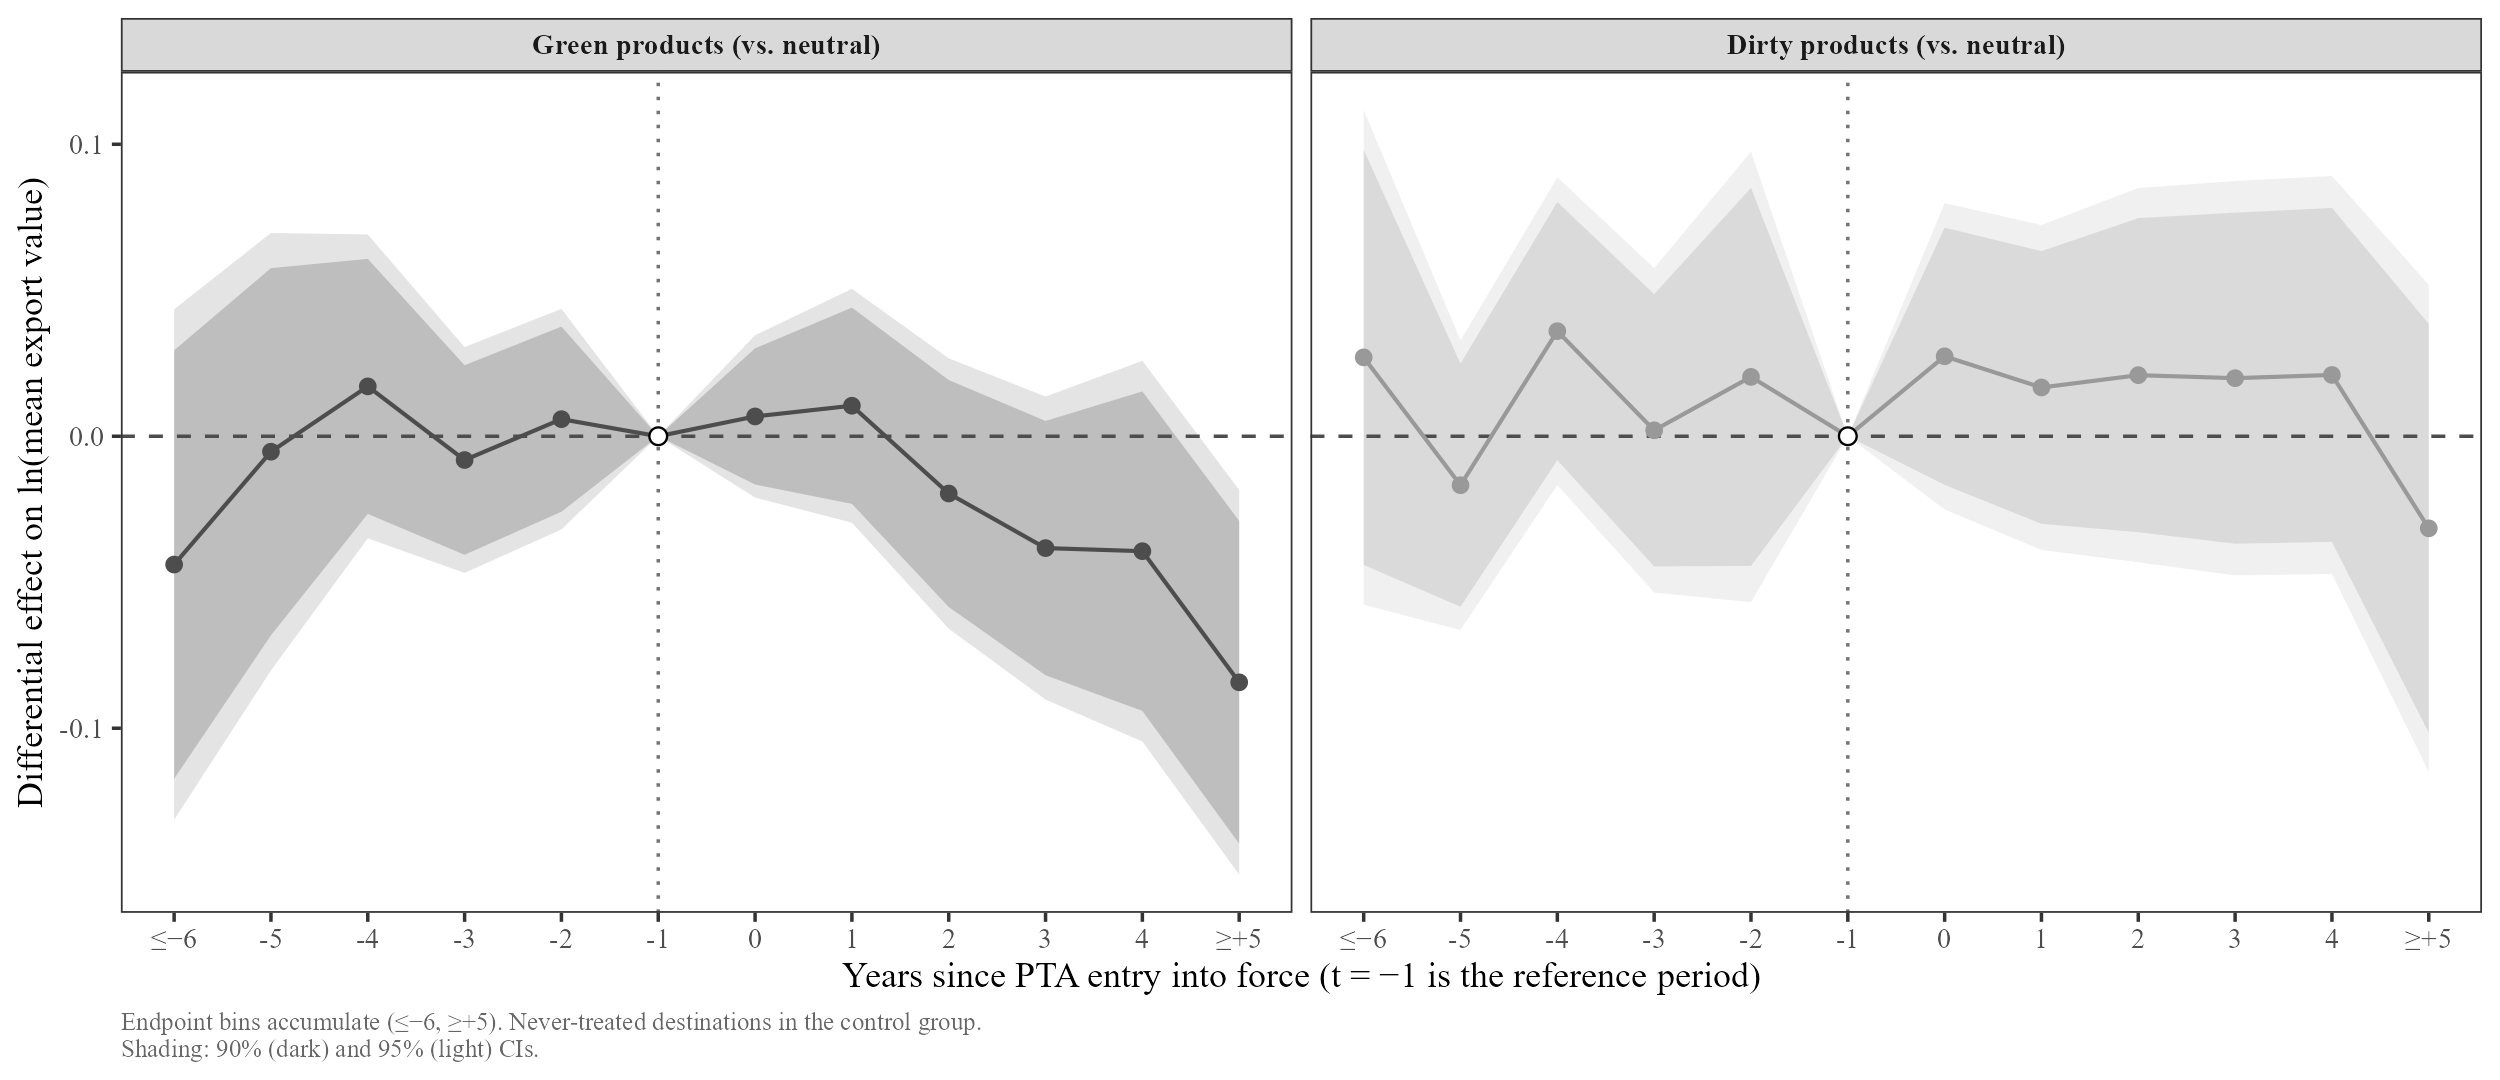
\includegraphics[width=\textwidth]{figures/eventstudy_collapsed_v3.png}
\begin{minipage}{\textwidth}\footnotesize
\emph{Notes:} Collapsed panel; FE $pd + dt + pt$; binary treatment, no depth control; destination-clustered 95\% confidence bands;
$t = -1$ is the reference period; endpoint bins accumulate. Coefficients are tabulated in Appendix
Table~\ref{tab:eventstudy_twfe}. Source: Chinese Customs Office; World Bank DTA Database.
\end{minipage}
\end{figure}

\FloatBarrier
\subsection{The extensive margin}\label{sec:extensive}

Everything above conditions on positive flows, so an agreement that created green exports to a market
previously served by none would leave no trace in it. Table~\ref{tab:ppml} estimates the same
interactions by Poisson pseudo-maximum likelihood on an HS6--destination--year grid completed with
zeros \citep{santossilva2006}, of which 7.9 million cells out of 8.2 survive the estimator's removal
of separated and singleton observations.

The green interaction is $+0.0015$ ($p = 0.74$) with the World Bank index and $+0.0001$ ($p = 0.95$)
with TREND. There is no trade creation to detect. The dirty interaction is $-0.030$ ($p = 0.057$) and
$+0.003$ ($p = 0.55$), marginal at best and, once again, only under one of the two codings --- the
same pattern the intensive margin produced, which is at least internally consistent.

One limitation deserves stating. This grid detects a product newly exported to a destination, not a
new firm beginning to export a product that other Chinese firms already ship there, which is a common
form of firm-level entry. The extensive margin is probed, not exhausted.

\input{Tabelle/tab_07_ppml}



% ============================================================================
\section{Conclusion}\label{sec:conclusion}
% ============================================================================

China's trade agreements did not shift the composition of its exports between 2000 and 2015.
On the green margin, the finding is a \emph{bounded null}: the coefficient is indistinguishable
from zero in both panels, under both provision codings, under both depth controls, on value,
quantity and unit value alike, and under three separate replacements of the comparison group.
It is robust to bootstrap and permutation inference, and it is bounded from above by roughly one
quarter of the reference estimate in the aggregate literature, on an indicative per-provision comparison. This is not a failure to reject.
It is a circumscribed statement about the absence of a specific effect --- the kind the
literature has documented elsewhere under different conditions.

On the dirty margin the finding is weaker and we state it as such. The coefficient is negative
almost everywhere and its magnitude is stable, but its statistical standing is not. Under the
World Bank measure of general agreement depth the wild cluster bootstrap takes it well clear of
conventional thresholds; under the DESTA measure it does not, because the two controls leave
different amounts of independent variation in environmental depth. Two further pieces of
evidence resolve the ambiguity in the same direction. The permutation test, which reassigns
whole agreement profiles and therefore does not depend on how well the depth control is
measured, returns $p$-values
between 0.15 and 0.38 in every variant. And the leave-one-out exercise shows that the point
estimate is stable across all 23 exclusions ($-0.0097$ to $-0.0133$) while the standard error
doubles or triples when one of two destinations is dropped --- and which two depends, again, on
the depth control. Precision, not the estimate, is what those destinations supply. We do not
read this as an identified composition effect, and we do not claim it is definitively absent
either: the honest summary is that the design cannot separate it from a placebo.

The central reading is about content. Environmental provisions affect trade when they are
specific, binding, and targeted at a product category --- \citet{abman2024} show this for
deforestation, \citet{brandi2020} for trade composition. China's chapters of this period
were thin and cooperation-heavy: the two WB sub-indices with a direct trade mechanism are
perfectly collinear in-sample and appear in only three treated country--years. The policy
implication is direct: a chapter in an agreement is not itself the instrument. What the
chapter contains is. This reading is an inference across studies, not a causal finding of
the present design: the current specification cannot separate the effect of provision
content from that of agreement selection within the Chinese PTA context.

Methodologically, the paper adds a cautionary case. With treatment concentrated across
roughly a dozen agreements, asymptotically significant composition effects can emerge and
dissolve under honest inference. Bootstrap, permutation, and leave-one-out --- applied not
as robustness appendices but as the primary mode of inference --- should be standard
practice for this class of design.

Three limitations should be noted. The preferential tariff rate was not obtainable. For the green margin its omission can only bias the estimate upward; for the dirty margin it is a genuine confounder, since the sectors we call dirty are those most often excluded from tariff liberalisation, and the negative dirty coefficient should be read with that in mind.
A continuous-dose estimator in the spirit of \citet{callaway2024} is not implemented; the
TWFE coefficient is a weighted average of cohort-specific effects, though the permutation
test is agnostic about this weighting. The extensive margin is probed at the
product--destination level: new firm entry into a destination where other Chinese firms
already export the same green product is not detected.

\printbibliography

% ============================================================================
\appendix
% ============================================================================

\section{Equivalence of the collapsed and firm-level panels}\label{app:pddt}

The collapsed panel aggregates firm--HS6--destination--year observations to
HS6--destination--year cells with outcome equal to the within-cell mean of log exports
and weights equal to cell counts. Under fixed effects $pd + dt + pt$ the weighted
cell-level regression is algebraically identical to the unweighted micro-level regression
under the same fixed effects. Verification to seven significant figures: the
EP$\times$green coefficient is $-0.0045685$ in both; the EP$\times$dirty coefficient is
$-0.011873$ in both. The result is exact up to floating-point precision and holds by
construction of the collapse and weights, not by approximation. It is what licenses the
reading of Section~\ref{sec:collapsed}: the gap between Tables~\ref{tab:fullpanel}
and~\ref{tab:collapsed} is a difference of fixed-effect structures, not of datasets.

\section{Treated destinations}\label{app:trattamento}

Table~\ref{tab:trattamento} lists the 25 destinations covered by a Chinese PTA, including Hong Kong and Macao, which the main sample excludes, their agreement entry years, and the maximum EP depth in the sample period for both the WB and TREND indices.

\begin{table}[htbp]
\centering
\footnotesize
\caption{Treated destinations: PTA entry-into-force year and environmental content}
\label{tab:trattamento}
\begin{threeparttable}
\begin{tabular}{llcc}
\toprule
Destination & Dataset code & Year of entry into force & Maximum EP depth \\
 & & & WB \quad / \quad TREND \\
\midrule
Bangladesh & 103 & 2002 & 1 \quad / \quad 1 \\
India & 111 & 2002 & 1 \quad / \quad 1 \\
South Korea & 133 & 2002 & 17 \quad / \quad 72 \\
Laos & 119 & 2002 & 6 \quad / \quad 4 \\
Sri Lanka & 134 & 2002 & 1 \quad / \quad 1 \\
Hong Kong & 110 & 2003 & 4 \quad / \quad 5 \\
Macao & 121 & 2003 & 5 \quad / \quad 5 \\
Brunei & 105 & 2005 & 6 \quad / \quad 4 \\
Cambodia & 107 & 2005 & 6 \quad / \quad 4 \\
Timor-Leste & 144 & 2005 & 6 \quad / \quad 4 \\
Indonesia & 112 & 2005 & 6 \quad / \quad 4 \\
Malaysia & 122 & 2005 & 6 \quad / \quad 4 \\
Myanmar & 106 & 2005 & 6 \quad / \quad 4 \\
Philippines & 129 & 2005 & 6 \quad / \quad 4 \\
Singapore & 132 & 2005 & 7 \quad / \quad 15 \\
Thailand & 136 & 2005 & 6 \quad / \quad 4 \\
Vietnam & 141 & 2005 & 6 \quad / \quad 4 \\
Chile & 412 & 2006 & 5 \quad / \quad 30 \\
Pakistan & 127 & 2007 & 3 \quad / \quad 12 \\
New Zealand & 609 & 2008 & 7 \quad / \quad 53 \\
Peru & 434 & 2010 & 12 \quad / \quad 47 \\
Costa Rica & 415 & 2011 & 4 \quad / \quad 50 \\
Iceland & 322 & 2014 & 6 \quad / \quad 28 \\
Switzerland & 331 & 2014 & 14 \quad / \quad 53 \\
Australia & 601 & 2015 & 3 \quad / \quad 24 \\
\midrule
\textbf{Total} & 25 destinations & & \\
\bottomrule
\end{tabular}
\begin{tablenotes}[flushleft]\footnotesize
\item \emph{Notes:} Each row is a destination covered by a Chinese PTA in force between 2000 and 2015. EP depth = count of environmental provisions according to two independent codings: World Bank (WB) and TREND. The 11 ASEAN destinations share the same agreement (2005) and therefore the same EP values; the truly distinct agreements are 14. Hong Kong and Macao excluded from the main sample due to their entrep\^ot function.
\item \textit{Source:} World Bank DTA Database; TREND Database.
\end{tablenotes}
\end{threeparttable}
\end{table}


\section{Inference: full bootstrap and permutation tables}\label{app:inference}

Table~\ref{tab:wcb} reports the wild cluster bootstrap $p$-values for the four headline
coefficients across both panels, both indices, and all four sample--depth variants;
Table~\ref{tab:perm} does the same for the permutation test on export value. Both are the
complete versions of the figures quoted in Sections~\ref{sec:fullpanel}
and~\ref{sec:collapsed}.

\input{Tabelle/tab_A02_wcb}

\begin{table}[htbp]
\centering
\footnotesize
\caption{Permutation test: 1,000 random reassignments of environmental content}
\label{tab:perm}
\begin{threeparttable}
\begin{tabular}{lcccc}
\toprule
 & (1) & (2) & (3) & (4) \\
\midrule
\multicolumn{5}{l}{\textit{Panel A --- WB index}} \\
\addlinespace
EP depth $\times$ Green: observed coefficient & -0.00457 & 0.00173 & -0.00433 & -0.00675 \\
\quad Permutation $p$-value & 0.597 & 0.897 & 0.480 & 0.465 \\
\quad Valid permutations & 1,000 & 1,000 & 1,000 & 1,000 \\
\addlinespace
EP depth $\times$ Dirty: observed coefficient & -0.01187 & -0.01887 & -0.01134 & -0.00820 \\
\quad Permutation $p$-value & 0.278 & 0.146 & 0.146 & 0.384 \\
\quad Valid permutations & 1,000 & 1,000 & 1,000 & 1,000 \\
\addlinespace
\multicolumn{5}{l}{\textit{Panel B --- TREND index}} \\
\addlinespace
EP count $\times$ Green: observed coefficient & 0.00181 & 0.00178 & 0.00161 & 0.00017 \\
\quad Permutation $p$-value & 0.160 & 0.468 & 0.316 & 0.929 \\
\quad Valid permutations & 1,000 & 1,000 & 1,000 & 1,000 \\
\addlinespace
EP count $\times$ Dirty: observed coefficient & 0.00035 & -0.00001 & -0.00025 & 0.00084 \\
\quad Permutation $p$-value & 0.817 & 0.996 & 0.904 & 0.788 \\
\quad Valid permutations & 1,000 & 1,000 & 1,000 & 1,000 \\
\addlinespace
\bottomrule
\end{tabular}
\begin{tablenotes}[flushleft]\footnotesize
\item \emph{Notes:} Columns: (1) Excl.\ HK/Macao, TotalDepth control; (2) Incl.\ HK/Macao, TotalDepth control; (3) Excl.\ HK/Macao, DESTA control; (4) Incl.\ HK/Macao, DESTA control. EP profiles (depth and entry years) randomly reassigned among the 23 treated destinations ($R = 1{,}000$); the $p$-value is the share of reassignments producing a coefficient at least as large in absolute value as the observed one. The 13 distinct EP profiles make the permutation distribution discrete.
\item \textit{Source:} Chinese Customs Office; World Bank DTA Database; TREND Database.
\end{tablenotes}
\end{threeparttable}
\end{table}


\section{Wild-cluster-bootstrap coefficient matrix}\label{app:matrice}

Table~\ref{tab:matrice} reports the wild-cluster-bootstrap $p$-value for the dirty-goods coefficient across all four sample--depth combinations (two Hong Kong and Macao stances $\times$ two depth controls), on both the collapsed panel and the full firm-level panel. Using the same bootstrap procedure for all cells makes the eight $p$-values directly comparable, and the pattern they show is the one discussed in Section~\ref{sec:collapsed}: the point estimate is uniformly negative, while significance tracks the choice of depth control rather than the sample.

\begin{table}[htbp]
\centering
\footnotesize
\caption{Summary: dirty-product coefficient across four specification variants, with common inference method}
\label{tab:matrice}
\begin{threeparttable}
\begin{tabular}{lcccc}
\toprule
 & (1) & (2) & (3) & (4) \\
\midrule
Collapsed panel: coefficient & -0.01187 & -0.01887 & -0.01134 & -0.00820 \\
\quad Bootstrap $p$-value & 0.072 & 0.005 & 0.047 & 0.195 \\
\addlinespace
\emph{Full panel}: coefficient & -0.00435 & -0.00409 & -0.00559 & -0.00574 \\
\quad Bootstrap $p$-value & 0.185 & 0.176 & 0.049 & 0.035 \\
\addlinespace
\bottomrule
\end{tabular}
\begin{tablenotes}[flushleft]\footnotesize
\item \emph{Notes:} Columns: (1) Excl.\ HK/Macao, TotalDepth control; (2) Incl.\ HK/Macao, TotalDepth control; (3) Excl.\ HK/Macao, DESTA control; (4) Incl.\ HK/Macao, DESTA control. Coefficient on $EP^{WB}_{dt} \times b_p$. All $p$-values are wild cluster bootstrap ($B = 9{,}999$), clustered by destination.
\item \textit{Source:} Chinese Customs Office; World Bank DTA Database; TREND Database.
\end{tablenotes}
\end{threeparttable}
\end{table}


\section{Saturation ladder}\label{app:ladder}

Tables~\ref{tab:ladder_wb} and~\ref{tab:ladder_trend} report the full version of the ladder summarised
in Table~\ref{tab:ladder_compact}, for all three outcomes and for both the baseline specification
without product-type interactions and the interacted specification. Two caveats apply to reading
across columns. First, iterative singleton removal differs across fixed-effect structures, so the
samples are not nested: $N$ ranges from 22.9 million (\textit{fpt}+\textit{fpd}) to 35.6 million
(\textit{fpt}+\textit{pd}), and the comparison therefore mixes the effect of the fixed effects with
the effect of the sample. Second, none of the four structures in these tables includes
firm--destination--year effects; the reference specification is reached only in column~(5) of
Table~\ref{tab:ladder_compact}. The structural argument for why a destination--year intercept absorbs
environmental depth entirely, and why the design is therefore built on composition rather than levels,
is made in Section~\ref{sec:strategy} and does not rest on these estimates.

\begin{table}[htbp]
\centering
\scriptsize
\setlength{\tabcolsep}{3pt}
\caption{Saturation ladder --- WB EP depth ($EP^{WB}_{dt}$)}
\label{tab:ladder_wb}
\begin{threeparttable}
\begin{tabular}{lcccccccc}
\toprule
 & \multicolumn{4}{c}{Baseline} & \multicolumn{4}{c}{Interaction ($g_p$, $b_p$)} \\
\cmidrule(lr){2-5}\cmidrule(lr){6-9}
 & (1) & (2) & (3) & (4) & (5) & (6) & (7) & (8) \\
\midrule
\multicolumn{9}{l}{\textit{Panel A --- $\ln x^{val}_{fpdt}$}} \\[3pt]
\quad $EP^{WB}_{dt}$ & 0.0031 & 0.0046* & 0.0001 & 0.0009 &  &  &  &  \\
 & (0.0025) & (0.0027) & (0.0033) & (0.0022) &  &  &  &  \\
\quad $EP^{WB}_{dt} \times g_p$ &  &  &  &  & 0.0018 & 0.0012 & 0.0060 & 0.0050 \\
 &  &  &  &  & (0.0050) & (0.0027) & (0.0050) & (0.0037) \\
\quad $EP^{WB}_{dt} \times b_p$ &  &  &  &  & $-$0.0037 & $-$0.0015 & 0.0058* & 0.0064** \\
 &  &  &  &  & (0.0150) & (0.0027) & (0.0031) & (0.0027) \\[3pt]
Observations & 29,477,365 & 35,607,036 & 22,927,402 & 29,473,145 & 29,477,365 & 35,607,036 & 22,927,402 & 29,473,145 \\
Adj.\ $R^2$ & 0.795 & 0.621 & 0.859 & 0.798 & 0.795 & 0.621 & 0.859 & 0.798 \\
\addlinespace[6pt]
\midrule
\multicolumn{9}{l}{\textit{Panel B --- $\ln x^{qua}_{fpdt}$}} \\[3pt]
\quad $EP^{WB}_{dt}$ & 0.0042 & 0.0033 & $-$0.0003 & 0.0012 &  &  &  &  \\
 & (0.0028) & (0.0028) & (0.0034) & (0.0023) &  &  &  &  \\
\quad $EP^{WB}_{dt} \times g_p$ &  &  &  &  & 0.0023 & 0.0032 & 0.0061 & 0.0053 \\
 &  &  &  &  & (0.0037) & (0.0026) & (0.0060) & (0.0038) \\
\quad $EP^{WB}_{dt} \times b_p$ &  &  &  &  & $-$0.0025 & $-$0.0006 & 0.0048 & 0.0058** \\
 &  &  &  &  & (0.0131) & (0.0028) & (0.0031) & (0.0025) \\[3pt]
Observations & 29,259,694 & 35,355,735 & 22,748,753 & 29,255,449 & 29,259,694 & 35,355,735 & 22,748,753 & 29,255,449 \\
Adj.\ $R^2$ & 0.871 & 0.749 & 0.911 & 0.873 & 0.871 & 0.749 & 0.911 & 0.873 \\
\addlinespace[6pt]
\midrule
\multicolumn{9}{l}{\textit{Panel C --- $\ln x^{uv}_{fpdt}$}} \\[3pt]
\quad $EP^{WB}_{dt}$ & $-$0.0010* & 0.0014*** & 0.0005*** & $-$0.0002 &  &  &  &  \\
 & (0.0005) & (0.0003) & (0.0002) & (0.0003) &  &  &  &  \\
\quad $EP^{WB}_{dt} \times g_p$ &  &  &  &  & 0.0001 & $-$0.0019 & 0.0002 & 0.0003 \\
 &  &  &  &  & (0.0016) & (0.0017) & (0.0016) & (0.0008) \\
\quad $EP^{WB}_{dt} \times b_p$ &  &  &  &  & $-$0.0012 & $-$0.0014** & 0.0005 & 0.0008 \\
 &  &  &  &  & (0.0026) & (0.0006) & (0.0006) & (0.0006) \\[3pt]
Observations & 29,259,686 & 35,355,728 & 22,748,748 & 29,255,441 & 29,259,686 & 35,355,728 & 22,748,748 & 29,255,441 \\
Adj.\ $R^2$ & 0.956 & 0.932 & 0.973 & 0.957 & 0.956 & 0.932 & 0.973 & 0.957 \\
\addlinespace[6pt]
\midrule
\quad $\theta_{fpd}$ & \checkmark &  & \checkmark & \checkmark & \checkmark &  & \checkmark & \checkmark \\
\quad $\theta_{pt}$ &  &  &  & \checkmark &  &  &  & \checkmark \\
\quad $\theta_{fpt}$ &  & \checkmark & \checkmark &  &  & \checkmark & \checkmark &  \\
\quad $\theta_{pd}$ &  & \checkmark &  &  &  & \checkmark &  &  \\
\quad $\theta_{t}$ & \checkmark &  &  &  & \checkmark &  &  &  \\
Clusters ($d$) & 231 & 232 & 231 & 231 & 231 & 232 & 231 & 231 \\
\bottomrule
\end{tabular}
\begin{tablenotes}[flushleft]\footnotesize
\item \textit{Notes:} Each column represents a different fixed-effects structure. Columns~(1)--(4) estimate the baseline $EP^{WB}_{dt}$ coefficient without product-type interactions. Columns~(5)--(8) decompose the EP effect by interacting with environmental ($g_p$) and pollution-intensive ($b_p$) product classifications. Hong Kong and Macao excluded. All specifications include the non-environmental depth control ($TD_{dt}$) and its interactions (not shown). Standard errors clustered at the destination level in parentheses. $^{*}$~$p<0.10$, $^{**}$~$p<0.05$, $^{***}$~$p<0.01$.
\item \textit{Source:} Chinese Customs Office; World Bank DTA Database.
\end{tablenotes}
\end{threeparttable}
\end{table}


\begin{table}[htbp]
\centering
\scriptsize
\setlength{\tabcolsep}{3pt}
\caption{Saturation ladder --- TREND EP count ($EP^{TR}_{dt}$)}
\label{tab:ladder_trend}
\begin{threeparttable}
\begin{tabular}{lcccccccc}
\toprule
 & \multicolumn{4}{c}{Baseline} & \multicolumn{4}{c}{Interaction ($g_p$, $b_p$)} \\
\cmidrule(lr){2-5}\cmidrule(lr){6-9}
 & (1) & (2) & (3) & (4) & (5) & (6) & (7) & (8) \\
\midrule
\multicolumn{9}{l}{\textit{Panel A --- $\ln x^{val}_{fpdt}$}} \\[3pt]
\quad $EP^{TR}_{dt}$ & 0.0004 & 0.0010** & 0.0002 & 0.0003 &  &  &  &  \\
 & (0.0005) & (0.0005) & (0.0006) & (0.0004) &  &  &  &  \\
\quad $EP^{TR}_{dt} \times g_p$ &  &  &  &  & $-$0.0013 & 0.0010 & 0.0021** & 0.0018** \\
 &  &  &  &  & (0.0010) & (0.0009) & (0.0009) & (0.0008) \\
\quad $EP^{TR}_{dt} \times b_p$ &  &  &  &  & $-$0.0049*** & 0.000029 & 0.0002 & 0.0009 \\
 &  &  &  &  & (0.0015) & (0.0007) & (0.0011) & (0.0008) \\[3pt]
Observations & 29,477,365 & 35,607,036 & 22,927,402 & 29,473,145 & 29,477,365 & 35,607,036 & 22,927,402 & 29,473,145 \\
Adj.\ $R^2$ & 0.795 & 0.621 & 0.859 & 0.798 & 0.795 & 0.621 & 0.859 & 0.798 \\
\addlinespace[6pt]
\midrule
\multicolumn{9}{l}{\textit{Panel B --- $\ln x^{qua}_{fpdt}$}} \\[3pt]
\quad $EP^{TR}_{dt}$ & 0.0005 & 0.0006 & 0.000047 & 0.0003 &  &  &  &  \\
 & (0.0005) & (0.0005) & (0.0006) & (0.0005) &  &  &  &  \\
\quad $EP^{TR}_{dt} \times g_p$ &  &  &  &  & $-$0.0007 & 0.0013 & 0.0025** & 0.0017** \\
 &  &  &  &  & (0.0009) & (0.0009) & (0.0010) & (0.0008) \\
\quad $EP^{TR}_{dt} \times b_p$ &  &  &  &  & $-$0.0034*** & 0.0002 & 0.0002 & 0.0008 \\
 &  &  &  &  & (0.0012) & (0.0007) & (0.0011) & (0.0007) \\[3pt]
Observations & 29,259,694 & 35,355,735 & 22,748,753 & 29,255,449 & 29,259,694 & 35,355,735 & 22,748,753 & 29,255,449 \\
Adj.\ $R^2$ & 0.871 & 0.749 & 0.911 & 0.873 & 0.871 & 0.749 & 0.911 & 0.873 \\
\addlinespace[6pt]
\midrule
\multicolumn{9}{l}{\textit{Panel C --- $\ln x^{uv}_{fpdt}$}} \\[3pt]
\quad $EP^{TR}_{dt}$ & $-$0.0001 & 0.0004*** & 0.0001*** & 0.000022 &  &  &  &  \\
 & (0.0001) & (0.0001) & (0.000047) & (0.000048) &  &  &  &  \\
\quad $EP^{TR}_{dt} \times g_p$ &  &  &  &  & $-$0.0004 & $-$0.0003 & $-$0.0002 & 0.0002 \\
 &  &  &  &  & (0.0003) & (0.0003) & (0.0003) & (0.0002) \\
\quad $EP^{TR}_{dt} \times b_p$ &  &  &  &  & $-$0.0015*** & $-$0.0003* & $-$0.000005 & 0.0002 \\
 &  &  &  &  & (0.0003) & (0.0001) & (0.0001) & (0.0001) \\[3pt]
Observations & 29,259,686 & 35,355,728 & 22,748,748 & 29,255,441 & 29,259,686 & 35,355,728 & 22,748,748 & 29,255,441 \\
Adj.\ $R^2$ & 0.956 & 0.932 & 0.973 & 0.957 & 0.956 & 0.932 & 0.973 & 0.957 \\
\addlinespace[6pt]
\midrule
\quad $\theta_{fpd}$ & \checkmark &  & \checkmark & \checkmark & \checkmark &  & \checkmark & \checkmark \\
\quad $\theta_{pt}$ &  &  &  & \checkmark &  &  &  & \checkmark \\
\quad $\theta_{fpt}$ &  & \checkmark & \checkmark &  &  & \checkmark & \checkmark &  \\
\quad $\theta_{pd}$ &  & \checkmark &  &  &  & \checkmark &  &  \\
\quad $\theta_{t}$ & \checkmark &  &  &  & \checkmark &  &  &  \\
Clusters ($d$) & 231 & 232 & 231 & 231 & 231 & 232 & 231 & 231 \\
\bottomrule
\end{tabular}
\begin{tablenotes}[flushleft]\footnotesize
\item \textit{Notes:} Each column represents a different fixed-effects structure. Columns~(1)--(4) estimate the baseline $EP^{TR}_{dt}$ coefficient without product-type interactions. Columns~(5)--(8) decompose the EP effect by interacting with environmental ($g_p$) and pollution-intensive ($b_p$) product classifications. Hong Kong and Macao excluded. All specifications include the non-environmental depth control ($TD_{dt}$) and its interactions (not shown). Standard errors clustered at the destination level in parentheses. $^{*}$~$p<0.10$, $^{**}$~$p<0.05$, $^{***}$~$p<0.01$.
\item \textit{Source:} Chinese Customs Office; World Bank DTA Database; TREND Database.
\end{tablenotes}
\end{threeparttable}
\end{table}


\section{Dynamics: event study and destination-specific trends}\label{app:dynamics}

Table~\ref{tab:eventstudy_twfe} tabulates the two-way fixed-effects event study plotted in
Figure~\ref{fig:es}. Pre-treatment coefficients are individually indistinguishable from zero on both
margins. The negative coefficient on the green interaction at $t = 5$ should be read with the caution
its position invites: the panel ends in 2015, so that bin covers the thinnest treated subsample and is
identified by the earliest cohorts alone. The binary event studies do not reproduce the negative dirty interaction of the dose specification: the post-entry dirty coefficients are positive in Table~\ref{tab:eventstudy_twfe} and in the Sun--Abraham aggregate ($+0.073$). The negative dose coefficient is therefore a contrast across agreements of different depth rather than a decline after entry within agreements; Appendix~\ref{app:dose} returns to this point.

\begin{table}[p]
\centering
\scriptsize
\setlength{\tabcolsep}{4pt}\renewcommand{\arraystretch}{0.92}
\caption{Event study (TWFE) --- EP leads and lags interacted with product type}
\label{tab:eventstudy_twfe}
\begin{threeparttable}
\begin{tabular}{lcccc}
\toprule
 & \multicolumn{2}{c}{Baseline sample} & \multicolumn{2}{c}{DESTA-coverage sample} \\
\cmidrule(lr){2-3}\cmidrule(lr){4-5}
Period & $1[t] \times g_p$ & $1[t] \times b_p$ & $1[t] \times g_p$ & $1[t] \times b_p$ \\
       & (1)             & (2)             & (3)             & (4)             \\
\midrule
\multicolumn{5}{l}{\textit{Pre-treatment leads (parallel trends test)}} \\[1pt]
$t\leq-6$ & $-0.044$        & $0.027$         & $-0.044$        & $0.027$         \\
       & $(0.045)$       & $(0.043)$       & $(0.045)$       & $(0.043)$       \\[1pt]
$t=-5$ & $-0.005$        & $-0.017$        & $-0.005$        & $-0.017$        \\
       & $(0.038)$       & $(0.025)$       & $(0.038)$       & $(0.025)$       \\[1pt]
$t=-4$ & $0.017$         & $0.036$         & $0.017$         & $0.036$         \\
       & $(0.027)$       & $(0.027)$       & $(0.027)$       & $(0.027)$       \\[1pt]
$t=-3$ & $-0.008$        & $0.002$         & $-0.008$        & $0.002$         \\
       & $(0.020)$       & $(0.028)$       & $(0.020)$       & $(0.028)$       \\[1pt]
$t=-2$ & $0.006$         & $0.020$         & $0.006$         & $0.020$         \\
       & $(0.019)$       & $(0.039)$       & $(0.019)$       & $(0.039)$       \\[1pt]
\midrule
\multicolumn{5}{l}{\textit{Reference period}} \\[1pt]
$t=-1$ & $0$             & $0$             & $0$             & $0$             \\[1pt]
\midrule
\multicolumn{5}{l}{\textit{Post-treatment lags}} \\[1pt]
$t=0$  & $0.007$         & $0.027$         & $0.007$         & $0.027$         \\
       & $(0.014)$       & $(0.027)$       & $(0.014)$       & $(0.027)$       \\[1pt]
$t=1$  & $0.010$         & $0.017$         & $0.010$         & $0.017$         \\
       & $(0.020)$       & $(0.028)$       & $(0.020)$       & $(0.028)$       \\[1pt]
$t=2$  & $-0.020$        & $0.021$         & $-0.020$        & $0.021$         \\
       & $(0.024)$       & $(0.033)$       & $(0.024)$       & $(0.033)$       \\[1pt]
$t=3$  & $-0.038$        & $0.020$         & $-0.038$        & $0.020$         \\
       & $(0.026)$       & $(0.034)$       & $(0.026)$       & $(0.034)$       \\[1pt]
$t=4$  & $-0.039$        & $0.021$         & $-0.040$        & $0.021$         \\
       & $(0.033)$       & $(0.035)$       & $(0.033)$       & $(0.035)$       \\[1pt]
$t\geq5$  & $-0.084^{**}$   & $-0.032$        & $-0.084^{**}$   & $-0.032$        \\
       & $(0.034)$       & $(0.043)$       & $(0.034)$       & $(0.043)$       \\[1pt]
\midrule
Observations   & 3,681,023 & 3,681,023 & 3,677,333 & 3,677,333 \\
Clusters ($d$) & 228       & 228       & 228       & 228       \\
\bottomrule
\end{tabular}
\begin{tablenotes}[flushleft]\footnotesize
\item \emph{Notes:} TWFE event study on the collapsed panel. Treatment is binary: $\mathbf{1}[\text{rel.\ time}=t]$ equals one for treated destinations $t$ years from PTA entry into force ($t=0$), and zero for never-treated destinations. The coefficients are $\mathbf{1}[\text{rel.\ time}=t] \times g_p$ (cols.\ 1, 3) and $\mathbf{1}[\text{rel.\ time}=t] \times b_p$ (cols.\ 2, 4), estimated jointly; EP depth does not enter, and no depth control is included. $t=-1$ is the omitted reference period; endpoint bins accumulate ($\leq -6$, $\geq +5$). FE: $pd + dt + pt$; weights: cell counts. Standard errors clustered at the destination level in parentheses. Columns (3)--(4) re-estimate on the sample used for the DESTA variants, which drops the one treated destination (Timor-Leste) not covered by DESTA; this is why they differ from columns (1)--(2) only at the fourth decimal.
\item Pre-treatment coefficients ($t \leq -2$) are all statistically indistinguishable from zero, supporting the parallel-trends assumption. The negative coefficient on $1[t] \times g_p$ at $t\geq5$ should be interpreted cautiously: the panel ends in 2015 and that bin covers the thinnest treated subsample.
\item $^{*}$~$p<0.10$, $^{**}$~$p<0.05$, $^{***}$~$p<0.01$ (asymptotic, destination-clustered).
\end{tablenotes}
\end{threeparttable}
\end{table}


\section{Sun--Abraham event study}\label{app:sunab}

Figure~\ref{fig:sunab} and Table~\ref{tab:sunab} report the interaction-weighted
\citep{sun2021} event study of the green and dirty versus neutral differential, estimated
on the destination-year composition gap.

A note on standard errors. The cohort shares used to aggregate group-specific effects are
themselves estimated from the data; \citet{sun2021} prescribe including that estimation
uncertainty in the variance. The \textsc{Stata} implementation does so; the \textsc{R}
implementation treats the shares as fixed weights.\footnote{The \textsc{Stata} estimates use \texttt{eventstudyinteract} \citep{sun2021}; the \textsc{R} estimates use the Sun--Abraham estimator in \texttt{fixest::sunab} \citep{berge2018}.} The two agree on coefficients to 15 significant
figures but disagree on standard errors. The degree of disagreement is informative: where
a single cohort identifies a period (so there are no shares to estimate), the ratio of
the two standard errors is exactly 1.00; where many cohorts contribute and their effects
are heterogeneous, the ratio reaches 3 to 4. The standard errors reported here are the
\textsc{Stata} ones, which reflect the full estimation uncertainty.

With these standard errors, no coefficient in the $[-10, +8]$ window is individually
distinguishable from zero on the green or dirty margin. The ATT is $-0.042$ ($p = 0.27$)
for the green gap and $+0.073$ ($p = 0.28$) for the dirty gap. Any apparent pre-trend in
the \textsc{R} output (the lead at $t = -6$ had $p = 0.001$ with fixed-weight standard errors)
reflects the treatment of cohort-share uncertainty, not a genuine pre-trend anomaly.

\begin{figure}[htbp]
\centering
\caption{Sun--Abraham interaction-weighted event study: green and dirty vs.\ neutral
gap at the destination--year level. 95\% confidence bands account for estimation
uncertainty in cohort shares. The window $[-10, +8]$ is shown; the estimates outside it rest on
one or two cohorts each.}
\label{fig:sunab}
\vspace{6pt}

\includegraphics[width=\textwidth]{figures/eventstudy_sunab_v3.png}
\end{figure}

\input{Tabelle/tab_A08_sunab}

\section{Destination-specific trends and pre-trend tests}\label{app:trends}

Table~\ref{tab:trends} reports the two trend specifications discussed in
Section~\ref{sec:dynamics}. Panels~A and~A$'$ add a linear trend for each destination interacted with
product type, estimated over the full sample period; Panels~B and~B$'$ estimate destination-specific
slopes on pre-treatment years only and project them forward before re-estimating on the detrended
outcome.

The only green coefficient in this appendix that survives the wild cluster bootstrap
appears here: the TREND green interaction under full-period trends, at $-0.0022$ with bootstrap
$p = 0.015$. Two considerations argue against taking it at face value. Trends estimated over the full
sample period absorb both pre- and post-treatment variation and can reverse the sign of treatment
coefficients when cohort dynamics are present \citep{wolfers2006}, and the late negative drift these
trends absorb is precisely the early-cohort artifact that the Sun--Abraham estimator identifies as
noise. Panels~A and~B re-estimate the interactions after removing destination-specific trends fitted on
pre-entry years only. The TREND green interaction becomes $+0.0073$ (bootstrap $p = 0.19$), the WB
dirty interaction $+0.063$ ($p = 0.61$): the detrended estimates are imprecise and, for dirty, of
the opposite sign, because most cohorts offer only two to four pre-entry years on which to fit a
slope. The variant therefore cannot adjudicate; the Wolfers argument above is what carries the
reading of the full-period trend result.

\begin{table}[p]
\centering
\scriptsize
\caption{Destination-specific trends and pre-trend tests (collapsed panel)}
\label{tab:trends}
\renewcommand{\arraystretch}{0.94}
\begin{threeparttable}
\begin{tabular}{lcccc}
\toprule
 & (1) & (2) & (3) & (4) \\
\midrule
\multicolumn{5}{l}{\textit{Panel A --- destination$\times$product-type linear trends (WB index)}} \\
EP depth $\times$ Green & -0.00510 & -0.00200 & 0.00084 & -0.00006 \\
 & (0.00360) & (0.00436) & (0.00434) & (0.00441) \\
 & [0.494] & [0.808] & [0.896] & [0.995] \\
EP depth $\times$ Dirty & -0.00825$^{*}$ & -0.00927$^{**}$ & -0.01030$^{***}$ & -0.00930$^{***}$ \\
 & (0.00423) & (0.00414) & (0.00239) & (0.00204) \\
 & [0.275] & [0.249] & [0.086] & [0.037] \\
\multicolumn{5}{l}{\textit{Panel A$'$ --- same specification, TREND index}} \\
EP count $\times$ Green & -0.00217$^{***}$ & -0.00214$^{***}$ & -0.00111$^{**}$ & -0.00153$^{***}$ \\
 & (0.00062) & (0.00061) & (0.00053) & (0.00049) \\
 & [0.015] & [0.018] & [0.218] & [0.074] \\
EP count $\times$ Dirty & -0.00137 & -0.00142 & -0.00231$^{***}$ & -0.00164$^{**}$ \\
 & (0.00115) & (0.00114) & (0.00066) & (0.00064) \\
 & [0.355] & [0.339] & [0.048] & [0.109] \\
\multicolumn{5}{l}{\textit{Panel B --- pre-trend test (WB index)}} \\
Pre-agreement slope, Green & 0.01732 & 0.00402 & 0.01719$^{*}$ & 0.02218 \\
 & (0.01295) & (0.01678) & (0.00997) & (0.01346) \\
\quad Bootstrap $p$-value & 0.678 & 0.705 & 0.543 & 0.497 \\
Pre-agreement slope, Dirty & 0.06292 & 0.06237 & 0.07109$^{**}$ & 0.07056$^{**}$ \\
 & (0.04393) & (0.03983) & (0.03161) & (0.03159) \\
\quad Bootstrap $p$-value & 0.610 & 0.515 & 0.416 & 0.410 \\
\multicolumn{5}{l}{\textit{Panel B$'$ --- pre-trend test (TREND index)}} \\
Pre-agreement slope, Green & 0.00728$^{*}$ & 0.00707 & 0.00775$^{*}$ & 0.00944$^{**}$ \\
 & (0.00438) & (0.00441) & (0.00428) & (0.00389) \\
\quad Bootstrap $p$-value & 0.189 & 0.199 & 0.173 & 0.090 \\
Pre-agreement slope, Dirty & 0.01512$^{**}$ & 0.01512$^{**}$ & 0.01839$^{***}$ & 0.01703$^{***}$ \\
 & (0.00728) & (0.00721) & (0.00596) & (0.00613) \\
\quad Bootstrap $p$-value & 0.293 & 0.301 & 0.164 & 0.243 \\
\bottomrule
\end{tabular}
\begin{tablenotes}[flushleft]\footnotesize
\item \emph{Notes:} Columns: (1) Excl.\ HK/Macao, TotalDepth control; (2) Incl.\ HK/Macao, TotalDepth control; (3) Excl.\ HK/Macao, DESTA control; (4) Incl.\ HK/Macao, DESTA control. Panels~A/A$'$: linear destination$\times$product-type trends estimated over the full sample period. Panels~B/B$'$: destination-specific slopes estimated on pre-treatment years only and projected forward. Standard errors in parentheses; wild cluster bootstrap $p$-values in brackets. $^{*}$~$p<0.10$, $^{**}$~$p<0.05$, $^{***}$~$p<0.01$.
\item \textit{Source:} Chinese Customs Office; World Bank DTA Database; TREND Database.
\end{tablenotes}
\end{threeparttable}
\end{table}


\section{Sub-index estimates on the collapsed panel}\label{app:subindices}

Table~\ref{tab:subindex} reports the sub-index estimates on the collapsed panel, the counterpart to
Table~\ref{tab:subindex_fullpanel} in the main text. Each column is a separate regression replacing
the aggregate index with one sub-index; the coefficients are not partial effects. The contrast between
the two tables follows the contrast between the two panels on the aggregate index: coefficients that
reach significance on the collapsed panel --- Green Liberalization and Green Market Access interacted
with dirty products --- are close to zero on the full panel, which locates them in the between-firm
channel that $\theta_{fdt}$ absorbs. See Section~\ref{sec:bundling} for interpretation.

\begin{table}[htbp]
\centering
\footnotesize
\setlength{\tabcolsep}{4pt}
\caption{Collapsed panel --- sub-index decomposition}
\label{tab:subindex}
\begin{threeparttable}
\begin{tabular}{lrrrrrrr}
\toprule
 & \multicolumn{2}{c}{WB sub-indices} & \multicolumn{5}{c}{TREND sub-indices} \\
\cmidrule(lr){2-3}\cmidrule(lr){4-8}
 & (1) & (2) & (3) & (4) & (5) & (6) & (7) \\
 & \shortstack{Green\\Lib.} & \shortstack{Enf.\\DSM} & \shortstack{Green\\Mkt.} & \shortstack{Enf.\\DSM} & Hard & Soft & \shortstack{Reg.\\Space} \\
\midrule
\multicolumn{8}{l}{\textit{Panel A --- Non-environmental depth control ($TD_{dt}$, World Bank)}} \\[3pt]
$EP_{\text{sub}} \times g_p$ & $-$0.0115 & $-$0.0048 & $-$0.0271 & 0.0042 & 0.0022 & 0.0132 & 0.0242$^{**}$ \\
                             & (0.0879) & (0.0394) & (0.0303) & (0.0148) & (0.0047) & (0.0121) & (0.0099) \\[6pt]
$EP_{\text{sub}} \times b_p$ & $-$0.0876$^{*}$ & 0.0067 & $-$0.0491$^{**}$ & $-$0.0052 & $-$0.0013 & 0.0019 & 0.0225$^{***}$ \\
                             & (0.0483) & (0.0525) & (0.0243) & (0.0140) & (0.0037) & (0.0108) & (0.0086) \\[6pt]
\quad $\theta_{pd}$ & \checkmark & \checkmark & \checkmark & \checkmark & \checkmark & \checkmark & \checkmark \\
\quad $\theta_{dt}$ & \checkmark & \checkmark & \checkmark & \checkmark & \checkmark & \checkmark & \checkmark \\
\quad $\theta_{pt}$ & \checkmark & \checkmark & \checkmark & \checkmark & \checkmark & \checkmark & \checkmark \\
\addlinespace[3pt]
Observations & 3,681,023 & 3,681,023 & 3,681,023 & 3,681,023 & 3,681,023 & 3,681,023 & 3,681,023 \\
Clusters ($d$) & 228 & 228 & 228 & 228 & 228 & 228 & 228 \\
\addlinespace[6pt]
\midrule
\multicolumn{8}{l}{\textit{Panel B --- DESTA depth control}} \\[3pt]
$EP_{\text{sub}} \times g_p$ & $-$0.0141 & $-$0.0105 & $-$0.0290 & 0.0032 & 0.0017 & 0.0132 & 0.0149 \\
                             & (0.0892) & (0.0280) & (0.0288) & (0.0160) & (0.0047) & (0.0131) & (0.0104) \\[6pt]
$EP_{\text{sub}} \times b_p$ & $-$0.1001$^{**}$ & $-$0.0197 & $-$0.0543$^{***}$ & $-$0.0086 & $-$0.0023 & $-$0.0015 & 0.0092 \\
                             & (0.0398) & (0.0343) & (0.0187) & (0.0115) & (0.0029) & (0.0101) & (0.0075) \\[6pt]
\quad $\theta_{pd}$ & \checkmark & \checkmark & \checkmark & \checkmark & \checkmark & \checkmark & \checkmark \\
\quad $\theta_{dt}$ & \checkmark & \checkmark & \checkmark & \checkmark & \checkmark & \checkmark & \checkmark \\
\quad $\theta_{pt}$ & \checkmark & \checkmark & \checkmark & \checkmark & \checkmark & \checkmark & \checkmark \\
\addlinespace[3pt]
Observations & 3,677,333 & 3,677,333 & 3,677,333 & 3,677,333 & 3,677,333 & 3,677,333 & 3,677,333 \\
Clusters ($d$) & 228 & 228 & 228 & 228 & 228 & 228 & 228 \\
\bottomrule
\end{tabular}
\begin{tablenotes}[flushleft]\footnotesize
\item \textit{Notes:} Collapsed panel (HS6--destination--year cells), excluding Hong Kong and Macao.
  Dependent variable: mean log export value ($\bar{y}_{pdt}$), weighted by cell size.
  Each column estimates a separate model replacing the aggregate EP index with one sub-index;
  the non-environmental depth control ($TD_{dt} \times g_p$ and $TD_{dt} \times b_p$) is included in all specifications but not shown.
  Fixed effects: product-destination ($\theta_{pd}$), destination-year ($\theta_{dt}$), product-year ($\theta_{pt}$).
  Standard errors clustered at the destination level in parentheses.
  $^{*}$~$p<0.10$, $^{**}$~$p<0.05$, $^{***}$~$p<0.01$.
\item WB sub-indices: (1)~Green Liberalization; (2)~Enforcement \& DSM.
  TREND sub-indices: (3)~Green Market Access; (4)~Enforcement \& DSM; (5)~Hard obligations;
  (6)~Soft obligations; (7)~Regulatory Space.
\end{tablenotes}
\end{threeparttable}
\end{table}


\begin{table}[htbp]
\centering
\caption{Composition of EP sub-indices}
\label{tab:subindex_composition}
\small
\begin{threeparttable}
\begin{tabular}{@{}p{3.8cm}cp{7.5cm}@{}}
\toprule
Sub-index & Source & Content \\
\midrule
\multicolumn{3}{@{}l}{\textit{Trade-mechanism sub-indices}} \\
\addlinespace
Green Liberalization & WB & Liberalization of trade in environmental goods and services (WB\_10: tariff reductions and removal of non-tariff barriers on green products) \\
\addlinespace
Standards Non-Regression & WB & Commitments not to lower domestic environmental standards to attract trade or investment (WB\_2, WB\_8, WB\_9); collinear with Green Liberalization in-sample, not estimated separately \\
\addlinespace
Green Market Access & TREND & Provisions facilitating market access for environmental goods (X7\_01\_01, X7\_01\_02\_01--02, X8\_09\_04) \\
\midrule
\multicolumn{3}{@{}l}{\textit{Enforcement sub-indices}} \\
\addlinespace
Enforcement \& DSM (WB) & WB & Dispute resolution and enforcement mechanisms specific to the environmental chapter (WB\_13--WB\_16) \\
\addlinespace
Enforcement \& DSM (TREND) & TREND & Environmental dispute settlement and enforcement procedures (X5\_*, X11\_*, X12\_*, X13\_*) \\
\midrule
\multicolumn{3}{@{}l}{\textit{Cooperation and regulatory sub-indices (no direct trade mechanism)}} \\
\addlinespace
Hard obligations & TREND & Obligations stated in binding terms (X2\_*, X5\_*, X10\_*, X14\_*, net of the soft-obligation provisions) \\
\addlinespace
Soft obligations & TREND & Cooperation and best-endeavour language (X1\_*, X7\_09, X5\_01\_02) \\
\addlinespace
Regulatory Space & TREND & Regulatory autonomy and policy-space clauses (X1\_07--X1\_09, X8\_*) \\
\bottomrule
\end{tabular}
\begin{tablenotes}\footnotesize
\item \emph{Notes:} All sub-indices are constructed here from the raw provision-level codings in the WB DTA and TREND databases; they are not variables native to either database. ``Trade-mechanism'' sub-indices contain provisions with an identifiable channel to trade flows. ``Cooperation and regulatory'' sub-indices cover provisions that, while environmentally relevant, lack a direct mechanism through which they could shift the product composition of exports. Each sub-index is a count of the relevant provisions present in a given agreement. Source: World Bank DTA Database; TREND Database.
\end{tablenotes}
\end{threeparttable}
\end{table}

\section{Hong Kong and Macao}\label{app:hkmo}

Hong Kong and Macao are excluded from the estimation samples in the main text. Both are covered by
Closer Economic Partnership Arrangements with the mainland, and both function as entrep\^ots: a large
share of what China ships to them is re-exported onward \citep{feenstra2004}, so a shipment recorded as
an export to Hong Kong is frequently not a shipment to a Hong Kong buyer. Including them adds two
treated destinations whose recorded flows are a composite of final demand and transit.

Tables~\ref{tab:fullpanel_inclHKMO} and~\ref{tab:collapsed_inclHKMO} re-estimate both main
specifications with the two territories included. On the green margin nothing changes. On the dirty
margin the collapsed-panel coefficient roughly doubles under the World Bank depth control, to
$-0.0189$ with a bootstrap $p$-value of 0.005, while the permutation $p$-value stays at 0.146 --- the
same divergence between the two tests documented in Section~\ref{sec:collapsed}, in a sharper form.
The leave-one-out rows for the two territories in Table~\ref{tab:loo_new} show that dropping Hong Kong
alone moves the coefficient from $-0.0189$ to $-0.0129$: of the 0.0070 increase relative to the
baseline of $-0.0119$, Hong Kong accounts for 0.0060, and Macao for almost none ($-0.0183$ when
dropped). This is the reason the entrep\^ot economies are held out of the baseline rather than a
robustness footnote.

\begin{table}[htbp]
\centering
\footnotesize
\caption{Full panel including Hong Kong and Macao --- triple-difference estimates}
\label{tab:fullpanel_inclHKMO}
\begin{threeparttable}
\begin{tabular}{lcccccc}
\toprule
 & \multicolumn{3}{c}{WB EP depth ($EP^{WB}_{dt}$)} & \multicolumn{3}{c}{TREND EP count ($EP^{TR}_{dt}$)} \\
\cmidrule(lr){2-4}\cmidrule(lr){5-7}
 & (1) & (2) & (3) & (4) & (5) & (6) \\
 & $\ln x^{val}_{fpdt}$ & $\ln x^{qua}_{fpdt}$ & $\ln x^{uv}_{fpdt}$ & $\ln x^{val}_{fpdt}$ & $\ln x^{qua}_{fpdt}$ & $\ln x^{uv}_{fpdt}$ \\
\midrule
\multicolumn{7}{l}{\textit{Panel A --- Non-environmental depth control ($TD_{dt}$, World Bank)}} \\[3pt]
$EP_{dt} \times g_p$ & $-$0.0009 & $-$0.0001 & $-$0.0004 & $-$0.0001 & $-$0.0001 & $-$0.0001 \\
 & (0.0036) & (0.0038) & (0.0013) & (0.0010) & (0.0011) & (0.0003) \\[2pt]
\quad Asymptotic $p$ & [0.804] & [0.984] & [0.734] & [0.913] & [0.960] & [0.847] \\
\quad Bootstrap $p$ & [0.833] & --- & --- & [0.919] & --- & --- \\[6pt]
$EP_{dt} \times b_p$ & $-$0.0041 & $-$0.0036 & $-$0.0008 & $-$0.0010 & $-$0.0008 & $-$0.0001 \\
 & (0.0024) & (0.0031) & (0.0010) & (0.0006) & (0.0008) & (0.0004) \\[2pt]
\quad Asymptotic $p$ & [0.094] & [0.236] & [0.451] & [0.112] & [0.321] & [0.836] \\
\quad Bootstrap $p$ & [0.176] & --- & --- & [0.142] & --- & --- \\[6pt]
\quad $\theta_{fpd}$ & \checkmark & \checkmark & \checkmark & \checkmark & \checkmark & \checkmark \\
\quad $\theta_{fdt}$ & \checkmark & \checkmark & \checkmark & \checkmark & \checkmark & \checkmark \\
\quad $\theta_{pt}$  & \checkmark & \checkmark & \checkmark & \checkmark & \checkmark & \checkmark \\
\addlinespace[3pt]
Observations & 23,560,110 & 23,334,037 & 23,334,027 & 23,560,110 & 23,334,037 & 23,334,027 \\
Clusters ($d$) & 227 & 227 & 227 & 227 & 227 & 227 \\
$R^2$ & 0.871 & 0.910 & 0.963 & 0.871 & 0.910 & 0.963 \\
\addlinespace[6pt]
\midrule
\multicolumn{7}{l}{\textit{Panel B --- DESTA depth control}} \\[3pt]
$EP_{dt} \times g_p$ & $-$0.0020 & $-$0.0016 & $-$0.0004 & $-$0.0004 & $-$0.0003 & $-$0.0001 \\
 & (0.0035) & (0.0032) & (0.0019) & (0.0009) & (0.0009) & (0.0004) \\[2pt]
\quad Asymptotic $p$ & [0.572] & [0.617] & [0.824] & [0.675] & [0.716] & [0.723] \\
\quad Bootstrap $p$ & [0.611] & --- & --- & [0.703] & --- & --- \\[6pt]
$EP_{dt} \times b_p$ & $-$0.0057** & $-$0.0076** & 0.0008 & $-$0.0014* & $-$0.0017* & 0.0002 \\
 & (0.0027) & (0.0031) & (0.0010) & (0.0007) & (0.0009) & (0.0003) \\[2pt]
\quad Asymptotic $p$ & [0.034] & [0.015] & [0.419] & [0.052] & [0.058] & [0.524] \\
\quad Bootstrap $p$ & [0.035] & --- & --- & [0.082] & --- & --- \\[6pt]
\quad $\theta_{fpd}$ & \checkmark & \checkmark & \checkmark & \checkmark & \checkmark & \checkmark \\
\quad $\theta_{fdt}$ & \checkmark & \checkmark & \checkmark & \checkmark & \checkmark & \checkmark \\
\quad $\theta_{pt}$  & \checkmark & \checkmark & \checkmark & \checkmark & \checkmark & \checkmark \\
\addlinespace[3pt]
Observations & 23,381,204 & 23,155,803 & 23,155,793 & 23,381,204 & 23,155,803 & 23,155,793 \\
Clusters ($d$) & 227 & 227 & 227 & 227 & 227 & 227 \\
$R^2$ & 0.871 & 0.911 & 0.963 & 0.871 & 0.911 & 0.963 \\
\bottomrule
\end{tabular}
\begin{tablenotes}[flushleft]\footnotesize
\item \textit{Notes:} Full firm-level panel, including Hong Kong and Macao. Columns~(1) and~(4): log export value ($\ln x^{val}_{fpdt}$). Columns~(2) and~(5): log export quantity ($\ln x^{qua}_{fpdt}$). Columns~(3) and~(6): log unit value ($\ln x^{uv}_{fpdt} = \ln x^{val}_{fpdt} - \ln x^{qua}_{fpdt}$). Quantity and unit-value regressions are estimated on the subset of observations with non-missing quantity data. All specifications include $TD_{dt} \times g_p$ and $TD_{dt} \times b_p$ controls (not shown). Panel~A uses non-environmental WB depth ($TD_{dt}$); Panel~B uses DESTA depth. Standard errors clustered at the destination level in parentheses. Wild cluster bootstrap ($B = 9{,}999$) $p$-values in brackets; ``---'' indicates bootstrap not available for this outcome. $^{*}$~$p<0.10$, $^{**}$~$p<0.05$, $^{***}$~$p<0.01$ (asymptotic).
\item \textit{Source:} Chinese Customs Office; World Bank DTA Database; TREND Database.
\end{tablenotes}
\end{threeparttable}
\end{table}


\begin{table}[htbp]
\centering
\footnotesize
\caption{Collapsed panel including Hong Kong and Macao --- triple-difference estimates}
\label{tab:collapsed_inclHKMO}
\begin{threeparttable}
\begin{tabular}{lcc}
\toprule
 & WB EP depth ($EP^{WB}_{dt}$) & TREND EP count ($EP^{TR}_{dt}$) \\
\cmidrule(lr){2-2}\cmidrule(lr){3-3}
 & (1) & (2) \\
 & $\ln x^{val}_{fpdt}$ & $\ln x^{val}_{fpdt}$ \\
\midrule
\multicolumn{3}{l}{\textit{Panel A --- Non-environmental depth control ($TD_{dt}$, World Bank)}} \\[3pt]
$EP_{dt} \times g_p$ & 0.0017 & 0.0018 \\
 & (0.0091) & (0.0018) \\[2pt]
\quad Asymptotic $p$ & [0.849] & [0.337] \\
\quad Bootstrap $p$ & [0.825] & [0.414] \\
\quad Permutation $p$ & [0.897] & [0.468] \\[6pt]
$EP_{dt} \times b_p$ & $-$0.0189*** & $-$0.00001 \\
 & (0.0061) & (0.0015) \\[2pt]
\quad Asymptotic $p$ & [0.002] & [0.995] \\
\quad Bootstrap $p$ & [0.005] & [0.995] \\
\quad Permutation $p$ & [0.146] & [0.996] \\[6pt]
\quad $\theta_{pd}$ & \checkmark & \checkmark \\
\quad $\theta_{dt}$ & \checkmark & \checkmark \\
\quad $\theta_{pt}$ & \checkmark & \checkmark \\
\addlinespace[3pt]
Observations & 3,769,187 & 3,769,187 \\
Clusters ($d$) & 230 & 230 \\
\addlinespace[6pt]
\midrule
\multicolumn{3}{l}{\textit{Panel B --- DESTA depth control}} \\[3pt]
$EP_{dt} \times g_p$ & $-$0.0067 & 0.0002 \\
 & (0.0048) & (0.0020) \\[2pt]
\quad Asymptotic $p$ & [0.157] & [0.931] \\
\quad Bootstrap $p$ & [0.484] & [0.949] \\
\quad Permutation $p$ & [0.465] & [0.929] \\[6pt]
$EP_{dt} \times b_p$ & $-$0.0082 & 0.0008 \\
 & (0.0043) & (0.0015) \\[2pt]
\quad Asymptotic $p$ & [0.055] & [0.575] \\
\quad Bootstrap $p$ & [0.195] & [0.635] \\
\quad Permutation $p$ & [0.384] & [0.788] \\[6pt]
\quad $\theta_{pd}$ & \checkmark & \checkmark \\
\quad $\theta_{dt}$ & \checkmark & \checkmark \\
\quad $\theta_{pt}$ & \checkmark & \checkmark \\
\addlinespace[3pt]
Observations & 3,759,733 & 3,759,733 \\
Clusters ($d$) & 230 & 230 \\
\bottomrule
\end{tabular}
\begin{tablenotes}[flushleft]\footnotesize
\item \textit{Notes:} Collapsed panel (product$\times$destination$\times$period cells, analytic weights), including Hong Kong and Macao. Dependent variable: log export value ($\ln x^{val}_{fpdt}$). All specifications include $TD_{dt} \times g_p$ and $TD_{dt} \times b_p$ controls (not shown). Panel~A uses non-environmental WB depth ($TD_{dt}$); Panel~B uses DESTA depth. Standard errors clustered at the destination level in parentheses. Wild cluster bootstrap ($B = 9{,}999$) $p$-values in brackets. Permutation $p$-values (treated-only design, $R = 1{,}000$). $^{*}$~$p<0.10$, $^{**}$~$p<0.05$, $^{***}$~$p<0.01$ (asymptotic).
\item \textit{Source:} Chinese Customs Office; World Bank DTA Database; TREND Database.
\end{tablenotes}
\end{threeparttable}
\end{table}


\section{Full robustness battery with standard errors}\label{app:robustfull}

Table~\ref{tab:robust-full} reproduces the full-panel robustness specifications with standard errors and asymptotic $p$-values for both the WB and TREND indices. The variants are: adding product--destination--year controls for tariffs, market concentration and antidumping exposure; dropping the eleven destinations covered by the ASEAN cohort (the ten members of the China--ASEAN agreement plus Timor-Leste, which the customs data group with them); re-including Hong Kong and Macao; restricting to products with common support across agreement and non-agreement destinations; and replacing the dependent variable with the green share of the firm's export basket to that destination.

A note on the tariff control. The tariff variable is the applied duty recorded in the customs data. It varies across partner destinations for the same HS6--year in 97.9 percent of product--year cells, so it is a destination-specific tariff faced by Chinese exporters rather than an import duty levied by China. Its average does not fall after PTA entry for partner destinations, which indicates that it records the MFN rate rather than the preferential rate; the preferential rate was not obtainable from these data. Two features limit what this costs. The tariff enters only this table and the CEM matching, not the headline estimates; and any tariff change common to all products shipped to a destination in a year is absorbed by $\theta_{fdt}$, so only product-specific variation contributes. If PTA negotiations cut tariffs more on green goods and the omitted preferential rate captured that cut, the effect would load onto the green interaction with a positive sign. The estimate is zero, so the omission works against finding a positive effect rather than toward it.

The dirty margin is exposed in the opposite direction. Pollution-intensive products --- steel,
chemicals, refined petroleum, paper --- are the sectors most often placed on partners' sensitive
lists, where tariffs fall later and less: under the ASEAN--China agreement up to 400 tariff lines per
member remained above 20 percent until 2012 and at 50 percent until 2015. If partners cut tariffs less
on dirty than on neutral products, dirty exports grow less than neutral ones after entry into force
and the dirty interaction turns negative with no role for the environmental chapter. The
non-environmental depth control cannot separate this, because within the ASEAN bloc environmental
and non-environmental depth are constant. We cannot rule this channel out with the data at hand; it
is the most economical alternative reading of the collapsed-panel dirty coefficient, and it is
consistent with the fact that the coefficient is carried by the medium-depth ASEAN cohort
(Appendix~\ref{app:dose}).

\begin{table}[htbp]
\centering
\footnotesize
\setlength{\tabcolsep}{4pt}
\caption{Robustness on the full panel: sample, control, and dependent-variable variants}
\label{tab:robust-full}
\begin{threeparttable}
\begin{tabular}{lccrc}
\toprule
Variant & $\times$ Green & $\times$ Dirty & Observations & $R^2$ \\
\midrule
\multicolumn{5}{l}{\textit{Panel A --- WB index}} \\
\addlinespace
Additional controls$^{a}$ & -0.00023 & -0.00600$^{**}$ & 19,286,638 & 0.8736 \\
 & (0.00296) & (0.00259) & & \\
 & [0.935] & [0.022] & & \\
\addlinespace
Excluding the ASEAN cohort (11 destinations) & -0.00252 & -0.00438$^{*}$ & 19,236,090 & 0.8719 \\
 & (0.00360) & (0.00223) & & \\
 & [0.482] & [0.051] & & \\
\addlinespace
Including Hong Kong and Macao & -0.00089 & -0.00409$^{*}$ & 23,560,110 & 0.8706 \\
 & (0.00360) & (0.00243) & & \\
 & [0.804] & [0.094] & & \\
\addlinespace
Common-support products only & -0.00225 & -0.00435$^{*}$ & 21,519,197 & 0.8734 \\
 & (0.00392) & (0.00223) & & \\
 & [0.566] & [0.052] & & \\
\addlinespace
PTA partners only, deep vs.\ shallow & -0.00222 & -0.00344 & 5,262,293 & 0.8839 \\
 & (0.00351) & (0.00289) & & \\
 & [0.534] & [0.246] & & \\
\addlinespace
Green share in firm's export basket & \multicolumn{2}{c}{-0.00010} & 13,345,132 & 0.8510 \\
 & \multicolumn{2}{c}{(0.00015)} & & \\
 & \multicolumn{2}{c}{[0.502]} & & \\
\midrule
\multicolumn{5}{l}{\textit{Panel B --- TREND index}} \\
\addlinespace
Additional controls$^{a}$ & +0.00039 & -0.00085 & 19,286,638 & 0.8736 \\
 & (0.00091) & (0.00068) & & \\
 & [0.669] & [0.209] & & \\
\addlinespace
Excluding the ASEAN cohort (11 destinations) & -0.00102 & -0.00183$^{**}$ & 19,236,090 & 0.8719 \\
 & (0.00102) & (0.00072) & & \\
 & [0.318] & [0.012] & & \\
\addlinespace
Including Hong Kong and Macao & -0.00011 & -0.00101 & 23,560,110 & 0.8706 \\
 & (0.00100) & (0.00063) & & \\
 & [0.913] & [0.112] & & \\
\addlinespace
Common-support products only & -0.00011 & -0.00090 & 21,519,197 & 0.8734 \\
 & (0.00099) & (0.00062) & & \\
 & [0.924] & [0.153] & & \\
\addlinespace
PTA partners only, deep vs.\ shallow & -0.00036 & -0.00061 & 5,262,293 & 0.8839 \\
 & (0.00100) & (0.00101) & & \\
 & [0.721] & [0.549] & & \\
\addlinespace
Green share in firm's export basket & \multicolumn{2}{c}{-0.00006$^{**}$} & 13,345,132 & 0.8510 \\
 & \multicolumn{2}{c}{(0.00003)} & & \\
 & \multicolumn{2}{c}{[0.043]} & & \\
\addlinespace
\bottomrule
\end{tabular}
\begin{tablenotes}[flushleft]\footnotesize
\item \emph{Notes:} Baseline variant (excl.\ HK/Macao, TotalDepth control). Estimated with \texttt{reghdfe}; fixed effects and clustering as in the main specification, except where noted.
\item $^{a}$ \textit{Additional controls}: applied tariff, product-level exporter concentration, and antidumping exposure.
\item \textit{ASEAN cohort}: the ten members of the China--ASEAN agreement plus Timor-Leste, which the customs data group with them.
\item \textit{Common support}: only products exported to both agreement and non-agreement destinations are retained. For the others, no observed comparison exists.
\item \textit{Green share in basket}: the dependent variable changes. Instead of export value, it is the share of the firm's revenue from green products to that destination. Fixed effects: firm$\times$destination and year.
\item Standard error in parentheses, $p$-value in brackets. $^{*}$ $p<0.10$, $^{**}$ $p<0.05$, $^{***}$ $p<0.01$.
\end{tablenotes}
\end{threeparttable}
\end{table}


\section{Alternative depth controls}\label{app:depthbounds}

Environmental depth and general agreement depth are strongly correlated, and
Section~\ref{sec:fullpanel} shows that the dirty coefficient's precision depends on which control is
used. Table~\ref{tab:depthbounds} varies the control across four alternatives on the collapsed panel:
none, aggregate World Bank TotalDepth, a version restricted to the 14 non-environmental areas most
correlated with EP content, and the DESTA index. On the green margin the point estimate moves within a
band of 0.0024 log points --- narrower than a single standard error --- stays negative throughout, and
every interval contains zero. Dropping the depth control altogether moves the coefficient away from
zero rather than toward it, which is what one expects if EP depth then also captures the effect of
overall agreement depth. The green null does not rest on the choice of depth control.

\input{Tabelle/tab_A18_depthbounds}

\section{Entry-into-force timing}\label{app:eif}

Section~\ref{sec:strategy} codes a destination as treated from the calendar year of entry into
force. Seven agreements enter in the second half of the year, and two of them --- Australia and
Korea, both 20 December 2015 --- fall in the panel's final year, so their treated year records
eleven days of exposure. Table~\ref{tab:eif} re-estimates the collapsed-panel specification under
six variants: the baseline; coding Korea and Australia's 2015 treatment variables at their
pre-entry (2014) values (A1); doing the same for all seven second-half entrants (A2); dropping
2015 entirely (B); dropping Korea and Australia outright (C); and treating single-provision
(depth-1) destinations as untreated, since a lone 1975 Bangkok Agreement provision is a weak claim
to a substantive environmental chapter (D). The WB dirty coefficient is estimated imprecisely
under every variant that touches the two 2015 entrants (A1, A2, B, C): the point estimate loses its
sign and its standard error roughly triples relative to the baseline, consistent with
Section~\ref{sec:strategy}'s observation that Korea and Australia carry a large share of the
identifying variation on that margin. The TREND dirty coefficient is small and imprecise in the
baseline and in D, but turns marginally significant ($p \approx 0.06$--$0.08$) and positive in
A1, A2, B and C --- the opposite sign from the WB result on the same subsample, which is a caution
against reading either index's dirty coefficient as robust to how the two 2015 entrants are coded.
The WB green coefficient is never distinguishable from zero. The TREND green coefficient tells a
different story: an imprecise zero in the baseline and D ($p = 0.32$ and $0.24$), it becomes
positive and precisely estimated ($p < 0.001$) in every variant that recodes or removes the two
2015 entrants (A1, A2, B, C). This is the reverse of what an omitted pre-existing trend would
produce, and it says that Korea and Australia's very deep, very late chapters pull the TREND green
estimate toward zero in the baseline rather than driving it; the coefficient the timing variants
recover is closer to a per-provision effect of the earlier, shallower chapters.

\begin{table}[htbp]
\centering
\footnotesize
\caption{Entry-into-force timing: robustness of the collapsed-panel estimates}
\label{tab:eif}
\begin{threeparttable}
\begin{tabular}{lcccc}
\toprule
 & \multicolumn{2}{c}{WB index} & \multicolumn{2}{c}{TREND index} \\
\cmidrule(lr){2-3}\cmidrule(lr){4-5}
Variant & EP$\times$green & EP$\times$dirty & EP$\times$green & EP$\times$dirty \\
\midrule
Baseline & $-0.0046$ & $-0.0119^{***}$ & $0.0018$ & $0.0004$ \\
         & $(0.0070)$ & $(0.0030)$ & $(0.0018)$ & $(0.0016)$ \\[4pt]
A1: Korea \& Australia 2015 coded pre-EIF & $0.0175$ & $-0.0059$ & $0.0052^{***}$ & $0.0030^{*}$ \\
         & $(0.0124)$ & $(0.0094)$ & $(0.0012)$ & $(0.0016)$ \\[4pt]
A2: all second-half-entry years coded pre-EIF & $0.0085$ & $-0.0088$ & $0.0050^{***}$ & $0.0032^{*}$ \\
         & $(0.0120)$ & $(0.0117)$ & $(0.0012)$ & $(0.0017)$ \\[4pt]
B: drop 2015 & $0.0100$ & $-0.0064$ & $0.0045^{***}$ & $0.0029^{*}$ \\
         & $(0.0145)$ & $(0.0113)$ & $(0.0012)$ & $(0.0016)$ \\[4pt]
C: drop Korea and Australia entirely & $0.0174$ & $-0.0055$ & $0.0052^{***}$ & $0.0030^{*}$ \\
         & $(0.0123)$ & $(0.0094)$ & $(0.0013)$ & $(0.0016)$ \\[4pt]
D: single-provision (depth 1) destinations coded untreated & $-0.0041$ & $-0.0120^{***}$ & $0.0021$ & $0.0005$ \\
         & $(0.0070)$ & $(0.0031)$ & $(0.0018)$ & $(0.0016)$ \\
\bottomrule
\end{tabular}
\begin{tablenotes}[flushleft]\footnotesize
\item \emph{Notes:} Collapsed panel, WB total depth control, destination clustering. A1 and A2 recode the treatment variables of the affected destination--years to their pre-entry (previous-year) values rather than dropping observations. Asymptotic standard errors in parentheses. Cluster counts and observation counts are within a few hundred cells of the baseline (3{,}681{,}023 cells, 228 clusters) except B (3{,}344{,}592 cells, 227 clusters, 2015 dropped) and C (3{,}573{,}947 cells, 226 clusters). $^{*}$~$p<0.10$, $^{**}$~$p<0.05$, $^{***}$~$p<0.01$ (asymptotic).
\item \textit{Source:} Chinese Customs Office; World Bank DTA Database; TREND Database.
\end{tablenotes}
\end{threeparttable}
\end{table}


\section{Dose bins}\label{app:dose}

Section~\ref{sec:strategy} treats environmental depth as a continuous dose, which imposes linearity
on the response rather than testing it. Table~\ref{tab:dosebins} replaces the continuous depth
control with three indicators for the current-year dose --- low (1--5 provisions), medium (6--7),
and high (8 or more) --- estimated against the never-treated destination--years. The bins are
grumous: eleven of the 23 treated destinations sit at exactly six provisions (the ASEAN bloc plus
Iceland), and only three destination--years exceed seven (Peru at 12, Switzerland at 14, Korea at 17
in 2015 only), so the high bin rests on one country per dose level and its standard error should be
read as uninformative rather than as evidence of a large effect. On the green margin every bin
coefficient is imprecise, and the one that clears the 10 percent threshold under the asymptotic
standard error (the low bin, $+0.064$) does not survive the wild cluster bootstrap ($p = 0.165$),
the same wedge the paper's main results show throughout with few treated clusters. On the dirty
margin the bins move in different directions --- positive in the low bin, negative and larger in
magnitude than the linear fit implies in the medium and high bins --- so the negative linear dirty
coefficient of Table~\ref{tab:collapsed} is better read as a contrast between the medium-depth ASEAN
cohort and the rest of the sample than as a per-provision slope; neither bin individually reaches
significance under the bootstrap. The dose-response evidence therefore does not support a stronger
reading of either margin than the linear specification already gives.

\begin{table}[htbp]
\centering
\footnotesize
\caption{Dose bins: the current-dose response is not linear}
\label{tab:dosebins}
\begin{threeparttable}
\begin{tabular}{lcccccc}
\toprule
 & \multicolumn{3}{c}{Green} & \multicolumn{3}{c}{Dirty} \\
\cmidrule(lr){2-4}\cmidrule(lr){5-7}
Fascia (dose corrente) & Coef. & Implied by linear fit & $p$ (WCB) & Coef. & Implied by linear fit & $p$ (WCB) \\
\midrule
Low (1--5, median 1)   & $0.0643^{*}$  & $-0.0046$ & $0.165$ & $0.0364$    & $-0.0119$ & $0.666$ \\
                        & $(0.0308)$    &           &         & $(0.0351)$  &           &         \\[4pt]
Medium (6--7, median 6) & $0.0403$      & $-0.0274$ & $0.608$ & $-0.1060$   & $-0.0712$ & $0.284$ \\
                        & $(0.0721)$    &           &         & $(0.0882)$  &           &         \\[4pt]
High (8+, median 12)   & $0.2717$      & $-0.0548$ & --- & $-0.1700$   & $-0.1425$ & --- \\
                        & $(0.1772)$    &           &         & $(0.2325)$  &           &         \\
\midrule
Countries & 9 & & & 13 & & 3 (high) \\
Country--years & 83 & \multicolumn{2}{c}{131} & \multicolumn{2}{c}{9} & \\
\bottomrule
\end{tabular}
\begin{tablenotes}[flushleft]\footnotesize
\item \emph{Notes:} Collapsed panel, weighted by cell size, FE $pd+dt+pt$, clustered by destination (228 clusters, 3{,}681{,}023 cells for every row). Bins are defined on the current-year WB total depth (never-treated destination--years are the omitted category). ``Implied by linear fit'' is the baseline linear coefficient (Table~\ref{tab:collapsed}, column WB) times the bin's median depth; the gap between it and the bin coefficient is the departure from linearity the design is built to detect. Standard errors in parentheses are asymptotic. $p$ (WCB): wild cluster bootstrap $p$-value (Rademacher weights, 9{,}999 replications), computed only for the low and medium bins, which have countries at more than one dose level within the bin; the high bin has one country per dose level (Peru 12, Switzerland 14, Korea 17, only in 2015) and a bootstrap adds no information the asymptotic standard error does not already convey. The low-bin green coefficient is significant under the asymptotic standard error ($p=0.038$) but not under the wild cluster bootstrap ($p=0.165$), the same wedge the main results show throughout with few treated clusters. $^{*}$~$p<0.10$ (asymptotic).
\item \textit{Source:} Chinese Customs Office; World Bank DTA Database; TREND Database.
\end{tablenotes}
\end{threeparttable}
\end{table}


\section{APEC versus OECD product classification}\label{app:apec}

Table~\ref{tab:apec} compares the estimates when the green product list is restricted to the 54 APEC Environmental Goods List codes \citep{sauvage2014} against the baseline using the 248 OECD CLEG codes. The APEC list is a strict subset of the OECD list, agreed politically in 2012 and much narrower in coverage. If the green null depended on which products are labelled environmental, the two columns would diverge; they do not.

\begin{table}[htbp]
\centering
\footnotesize
\caption{Alternative environmental-good definition: OECD list vs.\ APEC list}
\label{tab:apec}
\begin{threeparttable}
\begin{tabular}{lcc}
\toprule
 & OECD list & APEC list \\
 & (used in this paper) & (54 codes) \\
\midrule
EP depth (WB) $\times$ Green & -0.00457 & 0.00501 \\
 & (0.00696) & (0.01266) \\
 & [0.512] & [0.693] \\
\addlinespace
EP count (TREND) $\times$ Green & 0.00181 & 0.00319 \\
 & (0.00182) & (0.00208) \\
 & [0.320] & [0.126] \\
\bottomrule
\end{tabular}
\begin{tablenotes}[flushleft]\footnotesize
\item \emph{Notes:} Collapsed panel, excl.\ HK/Macao, TotalDepth control. The APEC Environmental Goods List (54 codes) replaces the OECD CLEG list (248 codes) used in the baseline. Standard errors in parentheses, $p$-values in brackets. $^{*}$~$p<0.10$, $^{**}$~$p<0.05$, $^{***}$~$p<0.01$.
\item \textit{Source:} Chinese Customs Office; World Bank DTA Database; TREND Database.
\end{tablenotes}
\end{threeparttable}
\end{table}


\section{CO$_2$ intensity as a continuous dirty measure}\label{app:co2}

The binary dirty indicator groups HS6 products into five pollution-intensive sectors, and a continuous
measure of emission intensity might tell a different story. We construct one from the replication data
of \citet{shapiro2021}, which reports China-specific CO$_2$ emission intensities for 47 EXIOBASE
industries.\footnote{\citet{shapiro2021} documents that most countries' tariff structures implicitly
subsidize pollution-intensive sectors and tax clean ones --- a systematic environmental bias that
environmental chapters are meant to work against.} HS6 products are mapped to ISIC3 divisions through
the same concordance used for the binary classification; unmatched codes, 9.5 percent of the panel,
are assigned the sample mean. The resulting measure validates against the existing trichotomy without
circularity: mean intensity is 0.0012 for dirty products, 0.0008 for neutral and 0.0006 for green,
monotonic in the expected direction.

Table~\ref{tab:co2} re-estimates the collapsed-panel specification with the standardized intensity in
place of the binary indicator. The interaction with the World Bank index is $-0.0026$ with a bootstrap
$p$-value of 0.71; with the TREND index it is $-0.0013$, asymptotically significant at $p = 0.011$ but
with a bootstrap $p$-value of 0.063. The continuous measure fades under robust inference the same way
the binary one does. It is tested on the collapsed panel only: re-estimating the interaction structure
on the full panel would require substantial additional computation, and the collapsed-panel test is
sufficient to establish that the continuous measure behaves like the binary indicator.

\begin{table}[htbp]
\centering
\footnotesize
\caption{CO$_2$ intensity \citep{shapiro2021} --- collapsed panel, triple-difference}
\label{tab:co2}
\begin{threeparttable}
\begin{tabular}{lcccc}
\toprule
 & \multicolumn{2}{c}{WB depth control ($TD_{dt}$)} & \multicolumn{2}{c}{DESTA depth control} \\
\cmidrule(lr){2-3}\cmidrule(lr){4-5}
 & (1) & (2) & (3) & (4) \\
 & Excl.\ HK/Macao & Incl.\ HK/Macao & Excl.\ HK/Macao & Incl.\ HK/Macao \\
\midrule
\multicolumn{5}{l}{\textit{Panel A --- WB EP depth ($EP^{WB}_{dt}$)}} \\[3pt]
$EP_{dt} \times g_p$ & $-$0.0050 & 0.0004 & $-$0.0025 & $-$0.0041 \\
 & (0.0070) & (0.0080) & (0.0049) & (0.0055) \\[2pt]
\quad Asymptotic $p$ & [0.472] & [0.956] & [0.613] & [0.455] \\
\quad Bootstrap $p$ & [0.544] & [0.961] & [0.797] & [0.797] \\[6pt]
$EP_{dt} \times \text{CO}_2$ & $-$0.0026 & $-$0.0049 & 0.0013 & 0.0028 \\
 & (0.0057) & (0.0064) & (0.0031) & (0.0031) \\[2pt]
\quad Asymptotic $p$ & [0.653] & [0.448] & [0.679] & [0.373] \\
\quad Bootstrap $p$ & [0.707] & [0.529] & [0.773] & [0.384] \\[6pt]
\midrule
\multicolumn{5}{l}{\textit{Panel B --- TREND EP count ($EP^{TR}_{dt}$)}} \\[3pt]
$EP_{dt} \times g_p$ & 0.0009 & 0.0009 & 0.0011 & $-$0.00002 \\
 & (0.0017) & (0.0017) & (0.0018) & (0.0017) \\[2pt]
\quad Asymptotic $p$ & [0.605] & [0.617] & [0.546] & [0.990] \\
\quad Bootstrap $p$ & [0.677] & [0.698] & [0.652] & [0.993] \\[6pt]
$EP_{dt} \times \text{CO}_2$ & $-$0.0013$^{**}$ & $-$0.0014$^{**}$ & $-$0.0008$^{**}$ & $-$0.0002 \\
 & (0.0005) & (0.0005) & (0.0004) & (0.0006) \\[2pt]
\quad Asymptotic $p$ & [0.011] & [0.012] & [0.032] & [0.779] \\
\quad Bootstrap $p$ & [0.063] & [0.056] & [0.083] & [0.817] \\[6pt]
\quad $\theta_{pd}$ & \checkmark & \checkmark & \checkmark & \checkmark \\
\quad $\theta_{dt}$ & \checkmark & \checkmark & \checkmark & \checkmark \\
\quad $\theta_{pt}$ & \checkmark & \checkmark & \checkmark & \checkmark \\
\addlinespace[3pt]
Observations & 3,681,023 & 3,769,187 & 3,677,333 & 3,759,733 \\
Clusters ($d$) & 228 & 230 & 228 & 230 \\
\bottomrule
\end{tabular}
\begin{tablenotes}[flushleft]\footnotesize
\item \textit{Notes:} Collapsed panel (product$\times$destination$\times$year cells, analytic weights).
  The binary dirty indicator is replaced by a continuous product-level CO$_2$ emission intensity from \citet{shapiro2021}, mapped to HS6 codes.
  $EP_{dt} \times g_p$ captures the differential effect on environmental goods;
  $EP_{dt} \times \text{CO}_2$ captures the marginal effect of a one-unit increase in CO$_2$ intensity.
  All specifications include $TD_{dt} \times g_p$ and $TD_{dt} \times \text{CO}_2$ controls (not shown).
  Columns~(1) and~(3) exclude Hong Kong and Macao; columns~(2) and~(4) include them.
  Standard errors clustered at the destination level in parentheses.
  Wild cluster bootstrap ($B = 9{,}999$) $p$-values in brackets.
  $^{*}$~$p<0.10$, $^{**}$~$p<0.05$, $^{***}$~$p<0.01$ (asymptotic).
\item \textit{Source:} Chinese Customs Office; World Bank DTA Database; TREND Database; \citet{shapiro2021}.
\end{tablenotes}
\end{threeparttable}
\end{table}


\section{Extended tables for the comparison-group subsamples}\label{app:subsamples}

Tables~\ref{tab:cprodhs4}, \ref{tab:cem} and~\ref{tab:deepshallow} report the three subsamples of
Table~\ref{tab:subsamples} in full: three outcomes, two provision codings and two depth controls each.
The synoptic table in the main text reports the export-value column of each under the wild cluster
bootstrap; these give the quantity and unit-value columns and the asymptotic $p$-values alongside.

\subsection{C-prod-HS4}\label{app:cprodhs4}
\begin{table}[htbp]
\centering
\footnotesize
\caption{C-prod-HS4 subsample --- triple-difference estimates}
\label{tab:cprodhs4}
\begin{threeparttable}
\begin{tabular}{lcccccc}
\toprule
 & \multicolumn{3}{c}{WB EP depth ($EP^{WB}_{dt}$)} & \multicolumn{3}{c}{TREND EP count ($EP^{TR}_{dt}$)} \\
\cmidrule(lr){2-4}\cmidrule(lr){5-7}
 & (1) & (2) & (3) & (4) & (5) & (6) \\
 & $\ln x^{val}_{fpdt}$ & $\ln x^{qua}_{fpdt}$ & $\ln x^{uv}_{fpdt}$ & $\ln x^{val}_{fpdt}$ & $\ln x^{qua}_{fpdt}$ & $\ln x^{uv}_{fpdt}$ \\
\midrule
\multicolumn{7}{l}{\textit{Panel A --- Non-environmental depth control ($TD_{dt}$, World Bank)}} \\[3pt]
$EP_{dt} \times g_p$ & $-$0.0009 & $-$0.0019 & 0.0005 & 0.0005 & 0.0001 & 0.0002 \\
 & (0.0051) & (0.0043) & (0.0007) & (0.0011) & (0.0010) & (0.0004) \\[2pt]
\quad Asymptotic $p$ & [0.858] & [0.665] & [0.471] & [0.680] & [0.906] & [0.689] \\
\quad Bootstrap $p$ & [0.860] & [0.662] & [0.421] & [0.730] & [0.916] & [0.713] \\[6pt]
$EP_{dt} \times b_p$ & 0.0066 & 0.0068 & $-$0.0017 & 0.0024 & 0.0033 & $-$0.0004 \\
 & (0.0090) & (0.0111) & (0.0070) & (0.0066) & (0.0059) & (0.0024) \\[2pt]
\quad Asymptotic $p$ & [0.469] & [0.541] & [0.807] & [0.714] & [0.581] & [0.860] \\
\quad Bootstrap $p$ & [0.435] & [0.562] & [0.857] & [0.734] & [0.591] & [0.866] \\[6pt]
\quad $\theta_{fpd}$ & \checkmark & \checkmark & \checkmark & \checkmark & \checkmark & \checkmark \\
\quad $\theta_{fdt}$ & \checkmark & \checkmark & \checkmark & \checkmark & \checkmark & \checkmark \\
\quad $\theta_{pt}$ & \checkmark & \checkmark & \checkmark & \checkmark & \checkmark & \checkmark \\
\addlinespace[3pt]
Observations & 3,772,855 & 3,745,788 & 3,745,788 & 3,772,855 & 3,745,788 & 3,745,788 \\
Clusters ($d$) & 215 & 215 & 215 & 215 & 215 & 215 \\
Adj.\ $R^2$ & 0.737 & 0.835 & 0.923 & 0.737 & 0.835 & 0.923 \\
\addlinespace[6pt]
\midrule
\multicolumn{7}{l}{\textit{Panel B --- DESTA depth control}} \\[3pt]
$EP_{dt} \times g_p$ & $-$0.0009 & $-$0.0032 & 0.0012 & 0.0004 & $-$0.0003 & 0.0003 \\
 & (0.0051) & (0.0042) & (0.0012) & (0.0013) & (0.0011) & (0.0004) \\[2pt]
\quad Asymptotic $p$ & [0.867] & [0.449] & [0.338] & [0.779] & [0.790] & [0.484] \\
\quad Bootstrap $p$ & [0.855] & [0.461] & [0.368] & [0.817] & [0.806] & [0.546] \\[6pt]
$EP_{dt} \times b_p$ & 0.0033 & $-$0.0059 & 0.0076 & 0.0015 & $-$0.0006 & 0.0022 \\
 & (0.0168) & (0.0182) & (0.0098) & (0.0040) & (0.0032) & (0.0025) \\[2pt]
\quad Asymptotic $p$ & [0.846] & [0.747] & [0.440] & [0.719] & [0.854] & [0.383] \\
\quad Bootstrap $p$ & [0.850] & [0.758] & [0.554] & [0.735] & [0.852] & [0.454] \\[6pt]
\quad $\theta_{fpd}$ & \checkmark & \checkmark & \checkmark & \checkmark & \checkmark & \checkmark \\
\quad $\theta_{fdt}$ & \checkmark & \checkmark & \checkmark & \checkmark & \checkmark & \checkmark \\
\quad $\theta_{pt}$ & \checkmark & \checkmark & \checkmark & \checkmark & \checkmark & \checkmark \\
\addlinespace[3pt]
Observations & 3,772,321 & 3,745,254 & 3,745,254 & 3,772,321 & 3,745,254 & 3,745,254 \\
Clusters ($d$) & 214 & 214 & 214 & 214 & 214 & 214 \\
Adj.\ $R^2$ & 0.737 & 0.835 & 0.923 & 0.737 & 0.835 & 0.923 \\
\bottomrule
\end{tabular}
\begin{tablenotes}[flushleft]\footnotesize
\item \textit{Notes:} C-prod-HS4 subsample: green products plus the non-green products in the 106 HS4 headings that contain at least one green code, so that each green product is compared with its four-digit neighbours. Full firm-level panel, excluding Hong Kong and Macao. All specifications include $TD_{dt} \times g_p$ and $TD_{dt} \times b_p$ controls (not shown). Panel~A uses non-environmental WB depth ($TD_{dt}$); Panel~B uses DESTA depth. Standard errors clustered at the destination level in parentheses. Wild cluster bootstrap ($B = 9{,}999$) $p$-values in brackets. $^{*}$~$p<0.10$, $^{**}$~$p<0.05$, $^{***}$~$p<0.01$ (asymptotic).
\item \textit{Source:} Chinese Customs Office; World Bank DTA Database; TREND Database.
\end{tablenotes}
\end{threeparttable}
\end{table}


\subsection{CEM-matched destinations}\label{app:cem}
\begin{table}[htbp]
\centering
\footnotesize
\caption{CEM destinations --- triple-difference estimates}
\label{tab:cem}
\begin{threeparttable}
\begin{tabular}{lcccccc}
\toprule
 & \multicolumn{3}{c}{WB EP depth ($EP^{WB}_{dt}$)} & \multicolumn{3}{c}{TREND EP count ($EP^{TR}_{dt}$)} \\
\cmidrule(lr){2-4}\cmidrule(lr){5-7}
 & (1) & (2) & (3) & (4) & (5) & (6) \\
 & $\ln x^{val}_{fpdt}$ & $\ln x^{qua}_{fpdt}$ & $\ln x^{uv}_{fpdt}$ & $\ln x^{val}_{fpdt}$ & $\ln x^{qua}_{fpdt}$ & $\ln x^{uv}_{fpdt}$ \\
\midrule
\multicolumn{7}{l}{\textit{Panel A --- Non-environmental depth control ($TD_{dt}$, World Bank)}} \\[3pt]
$EP_{dt} \times g_p$ & $-$0.0023 & $-$0.0014 & $-$0.0003 & $-$0.0006 & $-$0.0002 & $-$0.0004 \\
 & (0.0037) & (0.0041) & (0.0016) & (0.0011) & (0.0012) & (0.0003) \\[2pt]
\quad Asymptotic $p$ & [0.543] & [0.734] & [0.837] & [0.576] & [0.857] & [0.201] \\
\quad Bootstrap $p$ & [0.610] & [0.824] & [0.887] & [0.609] & [0.878] & [0.241] \\[6pt]
$EP_{dt} \times b_p$ & $-$0.0041* & $-$0.0042 & $-$0.0002 & $-$0.0011 & $-$0.0006 & $-$0.0004 \\
 & (0.0024) & (0.0034) & (0.0013) & (0.0007) & (0.0010) & (0.0003) \\[2pt]
\quad Asymptotic $p$ & [0.098] & [0.214] & [0.868] & [0.140] & [0.541] & [0.308] \\
\quad Bootstrap $p$ & [0.251] & [0.544] & [0.928] & [0.204] & [0.610] & [0.403] \\[6pt]
\quad $\theta_{fpd}$ & \checkmark & \checkmark & \checkmark & \checkmark & \checkmark & \checkmark \\
\quad $\theta_{fdt}$ & \checkmark & \checkmark & \checkmark & \checkmark & \checkmark & \checkmark \\
\quad $\theta_{pt}$ & \checkmark & \checkmark & \checkmark & \checkmark & \checkmark & \checkmark \\
\addlinespace[3pt]
Observations & 13,992,396 & 13,858,213 & 13,858,206 & 13,992,396 & 13,858,213 & 13,858,206 \\
Clusters ($d$) & 57 & 57 & 57 & 57 & 57 & 57 \\
Adj.\ $R^2$ & 0.742 & 0.815 & 0.921 & 0.742 & 0.815 & 0.921 \\
\addlinespace[6pt]
\midrule
\multicolumn{7}{l}{\textit{Panel B --- DESTA depth control}} \\[3pt]
$EP_{dt} \times g_p$ & $-$0.0016 & $-$0.0016 & 0.0000 & $-$0.0005 & $-$0.0003 & $-$0.0003 \\
 & (0.0034) & (0.0035) & (0.0019) & (0.0011) & (0.0011) & (0.0005) \\[2pt]
\quad Asymptotic $p$ & [0.648] & [0.644] & [0.980] & [0.655] & [0.783] & [0.567] \\
\quad Bootstrap $p$ & [0.676] & [0.737] & [0.978] & [0.676] & [0.815] & [0.683] \\[6pt]
$EP_{dt} \times b_p$ & $-$0.0043* & $-$0.0055* & 0.0001 & $-$0.0013* & $-$0.0011 & $-$0.0002 \\
 & (0.0024) & (0.0030) & (0.0013) & (0.0007) & (0.0009) & (0.0003) \\[2pt]
\quad Asymptotic $p$ & [0.081] & [0.071] & [0.938] & [0.091] & [0.194] & [0.478] \\
\quad Bootstrap $p$ & [0.121] & [0.180] & [0.981] & [0.125] & [0.255] & [0.607] \\[6pt]
\quad $\theta_{fpd}$ & \checkmark & \checkmark & \checkmark & \checkmark & \checkmark & \checkmark \\
\quad $\theta_{fdt}$ & \checkmark & \checkmark & \checkmark & \checkmark & \checkmark & \checkmark \\
\quad $\theta_{pt}$ & \checkmark & \checkmark & \checkmark & \checkmark & \checkmark & \checkmark \\
\addlinespace[3pt]
Observations & 13,992,396 & 13,858,213 & 13,858,206 & 13,992,396 & 13,858,213 & 13,858,206 \\
Clusters ($d$) & 57 & 57 & 57 & 57 & 57 & 57 \\
Adj.\ $R^2$ & 0.742 & 0.815 & 0.921 & 0.742 & 0.815 & 0.921 \\
\bottomrule
\end{tabular}
\begin{tablenotes}[flushleft]\footnotesize
\item \textit{Notes:} CEM-matched destinations subsample. Full firm-level panel, excluding Hong Kong and Macao. Columns~(1) and~(4): log export value ($\ln x^{val}_{fpdt}$). Columns~(2) and~(5): log export quantity ($\ln x^{qua}_{fpdt}$). Columns~(3) and~(6): log unit value ($\ln x^{uv}_{fpdt}$). Quantity and unit-value regressions estimated on the subset with non-missing quantity data. All specifications include $TD_{dt} \times g_p$ and $TD_{dt} \times b_p$ controls (not shown). Panel~A uses non-environmental WB depth ($TD_{dt}$); Panel~B uses DESTA depth. Standard errors clustered at the destination level in parentheses. Wild cluster bootstrap ($B = 9{,}999$) $p$-values in brackets. $^{*}$~$p<0.10$, $^{**}$~$p<0.05$, $^{***}$~$p<0.01$ (asymptotic).
\item \textit{Source:} Chinese Customs Office; World Bank DTA Database; TREND Database.
\end{tablenotes}
\end{threeparttable}
\end{table}


\subsection{Deep versus shallow agreements}\label{app:deepshallow}
\begin{table}[htbp]
\centering
\footnotesize
\caption{Deep vs.\ shallow agreements --- triple-difference estimates}
\label{tab:deepshallow}
\begin{threeparttable}
\begin{tabular}{lcccccc}
\toprule
 & \multicolumn{3}{c}{WB EP depth ($EP^{WB}_{dt}$)} & \multicolumn{3}{c}{TREND EP count ($EP^{TR}_{dt}$)} \\
\cmidrule(lr){2-4}\cmidrule(lr){5-7}
 & (1) & (2) & (3) & (4) & (5) & (6) \\
 & $\ln x^{val}_{fpdt}$ & $\ln x^{qua}_{fpdt}$ & $\ln x^{uv}_{fpdt}$ & $\ln x^{val}_{fpdt}$ & $\ln x^{qua}_{fpdt}$ & $\ln x^{uv}_{fpdt}$ \\
\midrule
\multicolumn{7}{l}{\textit{Panel A --- Non-environmental depth control ($TD_{dt}$, World Bank)}} \\[3pt]
$EP_{dt} \times g_p$ & $-$0.0022 & $-$0.0013 & $-$0.0004 & $-$0.0004 & $-$0.0001 & $-$0.0002 \\
 & (0.0035) & (0.0036) & (0.0011) & (0.0010) & (0.0010) & (0.0002) \\[2pt]
\quad Asymptotic $p$ & [0.534] & [0.712] & [0.748] & [0.721] & [0.903] & [0.392] \\
\quad Bootstrap $p$ & [0.585] & [0.817] & [0.708] & [0.751] & [0.919] & [0.305] \\[6pt]
$EP_{dt} \times b_p$ & $-$0.0034 & $-$0.0034 & $-$0.0005 & $-$0.0006 & $-$0.0004 & $-$0.0003 \\
 & (0.0029) & (0.0034) & (0.0008) & (0.0010) & (0.0012) & (0.0003) \\[2pt]
\quad Asymptotic $p$ & [0.246] & [0.330] & [0.572] & [0.549] & [0.712] & [0.389] \\
\quad Bootstrap $p$ & [0.499] & [0.601] & [0.771] & [0.739] & [0.785] & [0.379] \\[6pt]
\quad $\theta_{fpd}$ & \checkmark & \checkmark & \checkmark & \checkmark & \checkmark & \checkmark \\
\quad $\theta_{fdt}$ & \checkmark & \checkmark & \checkmark & \checkmark & \checkmark & \checkmark \\
\quad $\theta_{pt}$ & \checkmark & \checkmark & \checkmark & \checkmark & \checkmark & \checkmark \\
\addlinespace[3pt]
Observations & 5,262,293 & 5,201,289 & 5,201,282 & 5,262,293 & 5,201,289 & 5,201,282 \\
Clusters ($d$) & 23 & 23 & 23 & 23 & 23 & 23 \\
Adj.\ $R^2$ & 0.751 & 0.844 & 0.932 & 0.751 & 0.844 & 0.932 \\
\addlinespace[6pt]
\midrule
\multicolumn{7}{l}{\textit{Panel B --- DESTA depth control}} \\[3pt]
$EP_{dt} \times g_p$ & $-$0.0016 & $-$0.0015 & $-$0.0002 & $-$0.0003 & $-$0.0002 & $-$0.0002 \\
 & (0.0032) & (0.0031) & (0.0018) & (0.0010) & (0.0009) & (0.0004) \\[2pt]
\quad Asymptotic $p$ & [0.619] & [0.633] & [0.915] & [0.776] & [0.832] & [0.624] \\
\quad Bootstrap $p$ & [0.616] & [0.727] & [0.910] & [0.784] & [0.857] & [0.715] \\[6pt]
$EP_{dt} \times b_p$ & $-$0.0042 & $-$0.0043 & $-$0.0007 & $-$0.0009 & $-$0.0008 & $-$0.0003 \\
 & (0.0025) & (0.0028) & (0.0009) & (0.0008) & (0.0009) & (0.0003) \\[2pt]
\quad Asymptotic $p$ & [0.113] & [0.141] & [0.431] & [0.253] & [0.401] & [0.294] \\
\quad Bootstrap $p$ & [0.173] & [0.294] & [0.755] & [0.386] & [0.492] & [0.336] \\[6pt]
\quad $\theta_{fpd}$ & \checkmark & \checkmark & \checkmark & \checkmark & \checkmark & \checkmark \\
\quad $\theta_{fdt}$ & \checkmark & \checkmark & \checkmark & \checkmark & \checkmark & \checkmark \\
\quad $\theta_{pt}$ & \checkmark & \checkmark & \checkmark & \checkmark & \checkmark & \checkmark \\
\addlinespace[3pt]
Observations & 5,260,451 & 5,199,451 & 5,199,444 & 5,260,451 & 5,199,451 & 5,199,444 \\
Clusters ($d$) & 23 & 23 & 23 & 23 & 23 & 23 \\
Adj.\ $R^2$ & 0.751 & 0.844 & 0.932 & 0.751 & 0.844 & 0.932 \\
\bottomrule
\end{tabular}
\begin{tablenotes}[flushleft]\footnotesize
\item \textit{Notes:} Deep vs.\ shallow agreements subsample: restricted to destinations with at least one deep PTA in force. Full firm-level panel, excluding Hong Kong and Macao. Columns~(1) and~(4): log export value ($\ln x^{val}_{fpdt}$). Columns~(2) and~(5): log export quantity ($\ln x^{qua}_{fpdt}$). Columns~(3) and~(6): log unit value ($\ln x^{uv}_{fpdt}$). Quantity and unit-value regressions estimated on the subset with non-missing quantity data. All specifications include $TD_{dt} \times g_p$ and $TD_{dt} \times b_p$ controls (not shown). Panel~A uses non-environmental WB depth ($TD_{dt}$); Panel~B uses DESTA depth. Standard errors clustered at the destination level in parentheses. Wild cluster bootstrap ($B = 9{,}999$) $p$-values in brackets. $^{*}$~$p<0.10$, $^{**}$~$p<0.05$, $^{***}$~$p<0.01$ (asymptotic).
\item \textit{Source:} Chinese Customs Office; World Bank DTA Database; TREND Database.
\end{tablenotes}
\end{threeparttable}
\end{table}


\section{Minimum detectable effects}\label{app:mde}

Table~\ref{tab:mde} reports the minimum detectable effect for the headline green and dirty coefficients under the empirical standard errors and the wild-cluster-bootstrap confidence intervals, expressed in both per-provision and per-standard-deviation terms. It is estimated on the collapsed panel, where the standard errors are larger than in the full panel, so the bounds it reports are looser than those quoted in Section~\ref{sec:fullpanel}.

The distinction it draws is worth stating explicitly. A null result can mean that the effect is absent or that the design cannot see it, and only an interval separates the two. On the green margin the bootstrap interval rules out effects larger than roughly three percent per provision at 95 percent confidence, and says nothing about anything smaller. For scale, \citet{brandi2020} find that one additional liberalising environmental provision raises
the green export share by about 17 percent (0.157 log points) in their aggregate bilateral panel of
developing-country exporters. The comparison is only indicative: their unit is a liberalising
provision, ours any environmental provision category, and their outcome a share rather than a
within-firm log gap. On that reading, the full-panel upper bound of Section~\ref{sec:fullpanel},
3.5 percent per provision, is roughly one quarter of their figure and the collapsed-panel bound in
Table~\ref{tab:mde}, 3.2 percent, roughly one fifth.

\begin{table}[htbp]
\centering
\footnotesize
\caption{How large an effect would the design need to detect it}
\label{tab:mde}
\begin{threeparttable}
\begin{tabular}{llcccc}
\toprule
Index & Margin & Asymptotic & Minimum detectable & Bootstrap CI & Bootstrap CI \\
 & & std.\ error & effect (1 s.d.) & half-width (1 s.d.) & (per unit) \\
\midrule
WB & Green & 0.0070 & 4.64\% & 6.00\% & [-1.85\%, 3.18\%] \\
WB & Dirty & 0.0030 & 1.97\% & 2.40\% & [-1.85\%, 0.17\%] \\
TREND & Green & 0.0018 & 4.16\% & 3.60\% & [-0.17\%, 0.71\%] \\
TREND & Dirty & 0.0016 & 3.65\% & 3.56\% & [-0.31\%, 0.56\%] \\
\bottomrule
\end{tabular}
\begin{tablenotes}[flushleft]\footnotesize
\item \emph{Notes:} Collapsed panel, excl.\ HK/Macao. Standard deviation of the EP indices weighted by cell size over all 3,773,498 cells of the collapsed panel, never-treated destinations included (2.38 for WB, 8.16 for TREND). Minimum detectable effect = $2.8 \times$ asymptotic standard error, which understates the true MDE by the same factor by which the bootstrap widens the interval; the bootstrap half-width column is the relevant bound.
\item \textit{Source:} Chinese Customs Office; World Bank DTA Database; TREND Database.
\end{tablenotes}
\end{threeparttable}
\end{table}


\end{document}
